\documentclass[parskip=full]{scrartcl}
\usepackage[T1]{fontenc}    % avoid garbled Unicode text in pdf
\usepackage[utf8]{inputenc} % use utf8 file encoding for TeX sources
\usepackage[german]{babel}  % german hyphenation, quotes, etc
\usepackage{hyperref}       % detailed hyperlink/pdf configuration
\hypersetup{                % ‘texdoc hyperref‘ for options
pdftitle={PSE: Entwicklung eines relationalen Debuggers - Pflichtenheft},%
,%
}
\usepackage{graphicx}       % provides commands for including figures
\usepackage{csquotes}       % provides \enquote{} macro for "quotes"
\usepackage[nonumberlist]{glossaries}     % provides glossary commands
\usepackage{enumitem}
\usepackage{xcolor}
\usepackage{lscape}
\newcommand\frage[1]{\textcolor{red}{#1}}


\font\myfont=cmr12 at 20pt

\title{
	\vspace{2cm}
	\myfont 
	Praxis der Softwareentwicklung:\\ 
	Entwicklung eines relationalen Debuggers\\
}
\subtitle{
	\vspace{1cm}
	\myfont
	Entwurfsdokument
}
\author{
	\vspace{1cm} \\
	Benedikt Wagner\\
	\texttt{udpto@student.kit.edu}
	\and \vspace{1cm} \\ Chiara Staudenmaier\\
	\texttt{uzhtd@student.kit.edu}
	\and Etienne Brunner\\
	\texttt{urmlp@student.kit.edu}
	\and Joana Plewnia\\
	\texttt{uhfpm@student.kit.edu} 
	\and Pascal Zwick\\
	\texttt{uyqpk@student.kit.edu}
	\and Ulla Scheler\\
	\texttt{ujuhe@student.kit.edu}
	\vspace{1cm}
	\and Betreuer: Mihai Herda, Michael Kirsten
	\vspace{4cm}
}


\begin{document}
\clearpage
\maketitle
\pagenumbering{gobble}
\newpage

\tableofcontents
\newpage
\pagenumbering{arabic}
%Eventuell Fußnoten generieren
\section{Einleitung}
%Einleitung mit grobem Überblick. Dieser Abschnitt soll an das Pflichtenheft anschließen.
Dieses Dokument dokumentiert die Ergebnisse der Entwurfsphase (\textit{28.11.-22.12.2017}) im Rahmen
des Moduls Praxis der Softwareentwicklung (PSE) am Lehrstuhl \enquote{Anwendungsorientierte formale Verifikation - Prof. Dr. Beckert} am Karlsruher Institut für Technologie (KIT).\\
Hierbei handelt es sich um den Entwurf des Produkts \textit{DIbugger}, welches im Pflichtenheft definiert wurde. 
Das Entwurfsdokument beschreibt die Paketeinteilung, Beschreibung der Klassen und Abläufe und genaue Spezifikation der Abhängigkeiten und Kernkomponenten. 
\\Die Implementierung während der Implementierungsphase (\textit{09.01.-02.02.2018}) wird anhand der Vorgaben in diesem Dokument durchgeführt. \\
Hierbei werden die aus der Softwaretechnik bekannten Prinzipien, wie etwa Geheimnisprinzip und Kapselungsprizip oder das Prinzip der losen Kopplung berücksichtigt. Wie genau die Einhaltung der Prinzipien sichergestellt wird, wird an den jeweiligen Stellen im Dokument erwähnt. 
\vspace{1cm}
\begin{figure}[!h]
\centering

\includegraphics[width=0.8\textwidth]{../Plichtenheft/logo_nongi.png}
\caption{Produktlogo}
\end{figure}

\newpage


\section{Paketeinteilung}\label{Packages} %eventuell fällt jemandem ein besserer Titel ein
%Paketdiagramm, Erläuterung der Einteilungsentscheidung, Schnittstellen

\subsection{Übersicht}

\begin{figure}[!h]
\centering
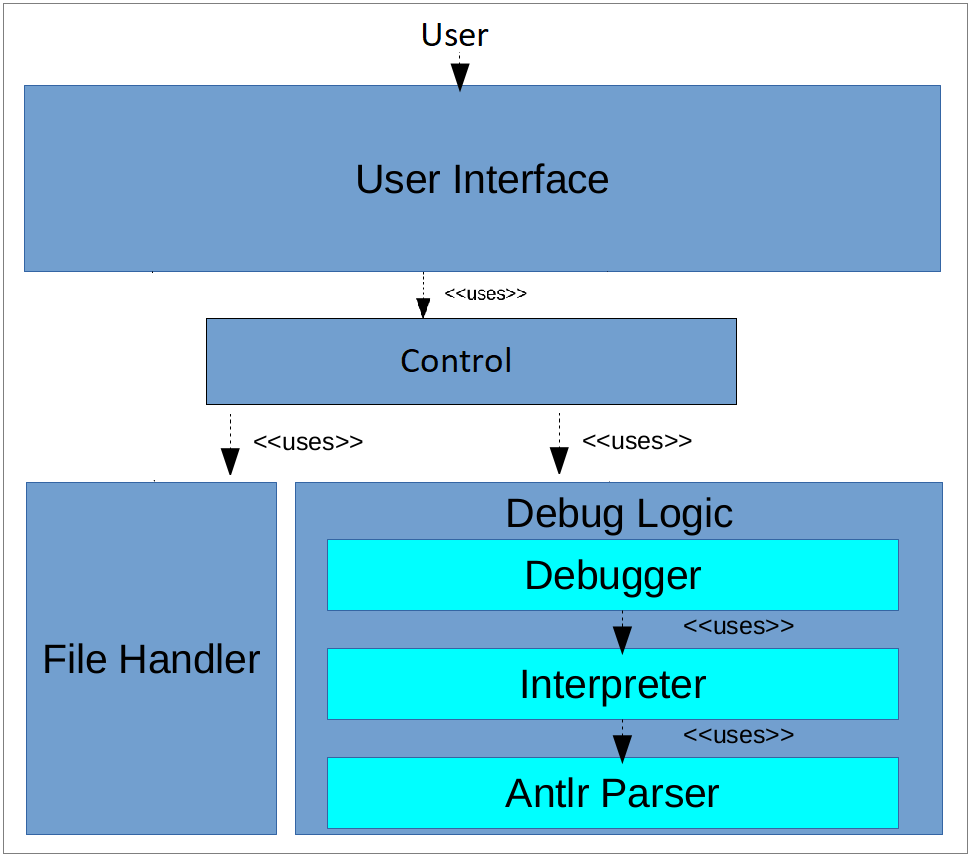
\includegraphics[scale=0.35]{../Plichtenheft/Architektur.png} \\
\caption{Architekturdiagramm}
\end{figure}
Das Produkt ist aufgeteilt in die Pakete \textit{Control}, \textit{UserInterface}, \textit{FileHandler} und \textit{DebugLogic}.
Die \textit{DebugLogic} besteht aus den Unterpaketen \textit{Debugger}, \textit{Interpreter} und
\textit{AntlrParser}.\\
Hierbei wird das Architekturmuster Model-View-Controller (MVC) eingesetzt, um einen flexiblen Programmentwurf zu ermöglichen und die Erweiterbarkeit des Produkts sicher zu stellen. Die Pakete \textit{DebugLogic} und \textit{FileHandler} sind hierbei das Modell, welches die darzustellenden Daten enthält. Das \textit{UserInterface} ist die Präsentationsschicht, welche Benutzereingaben annimmt und die darzustellenden Werte über ein Beobachtermuster erhält. Die Steuerung, welche Benutzereingaben von der Präsentationsschicht erhält und diese auswertet, wird vom \textit{Control}-Paket bereitgestellt. \\
Alle Pakete stellen ihre Funktionalität über Fassadenklassen nach außen zur Verfügung (siehe Abbildung \ref{fig:fassaden}). Die genauen Schnittstellen sind also durch diese Klassen definiert.

\newpage

\begin{landscape}

\begin{figure}[!h]
\centering
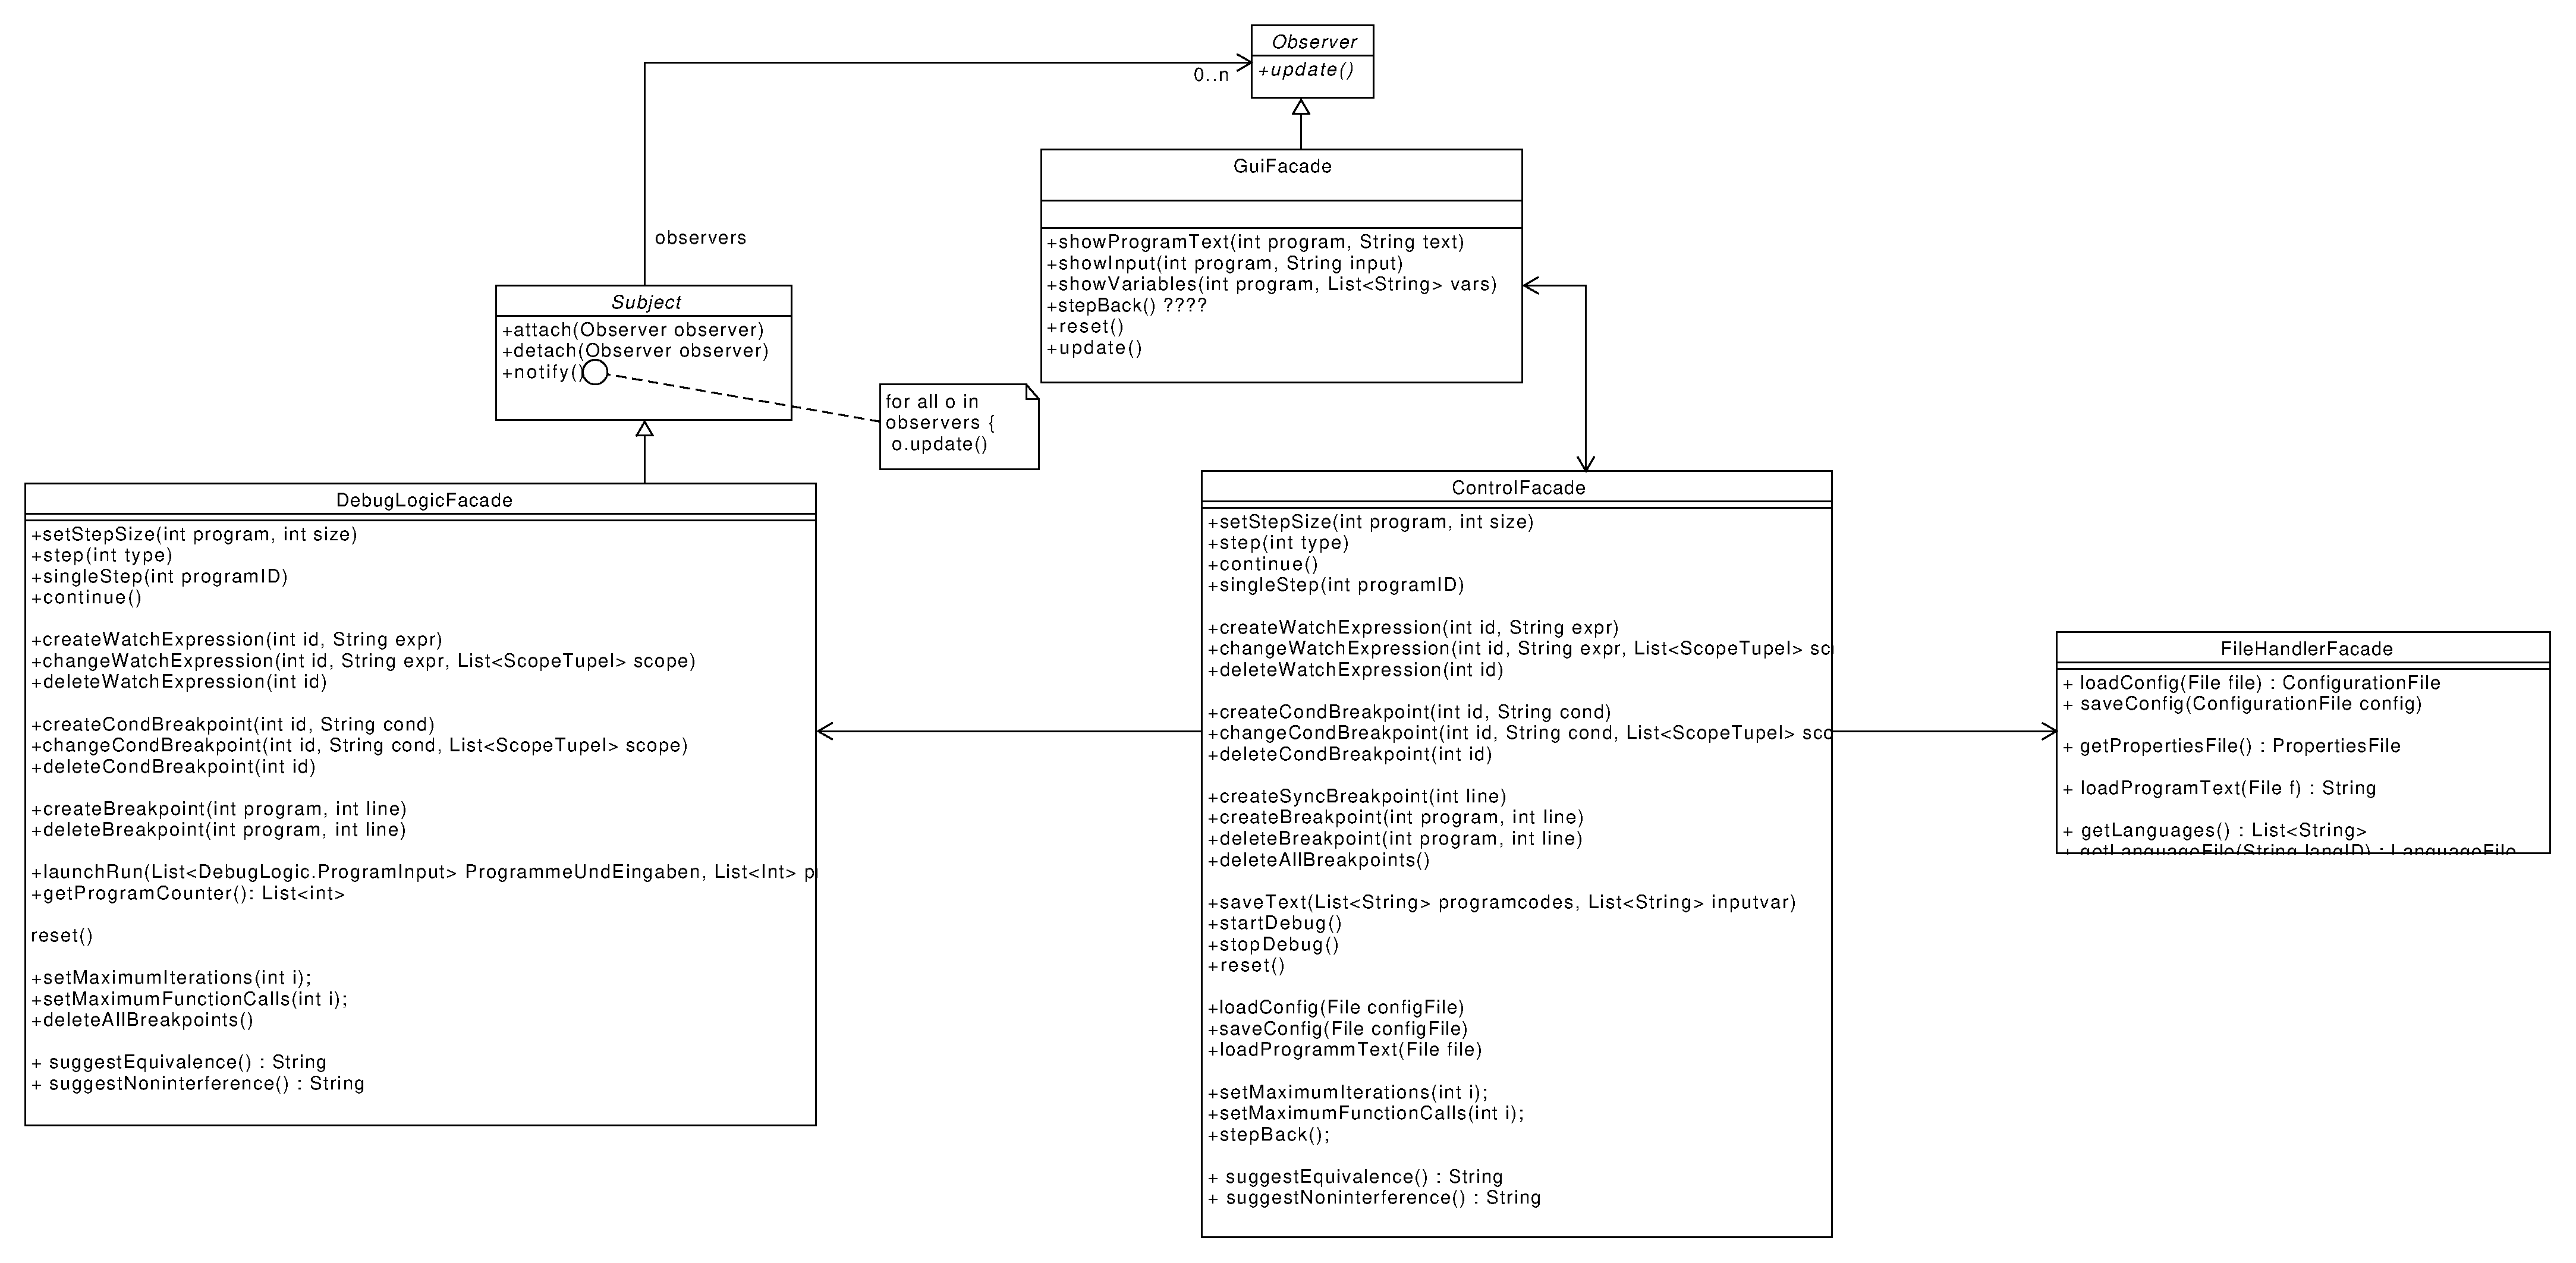
\includegraphics[scale=0.4]{diagrammIdeenUmlet/fassaden.pdf}
\caption{Die Schnittstellen der Pakete durch Fassaden dargestellt}
\label{fig:fassaden}
\end{figure}
\end{landscape}

\newpage

\subsection{User Interface}
\paragraph{Aufgaben} Das Paket \textit{UserInterface} stellt die Möglichkeit zur Kommunikation des Nutzers mit dem Produkt dar. Hierbei dient dieses Paket als View Teil des MVC-Konzepts.
\paragraph{Schnittstellen} 
\begin{itemize}
\item Angebotene Schnittstellen:\\
Es wird eine Fassade angeboten, welche es ermöglicht, Variablen, Programmtexte und Eingaben anzuzeigen.
\item Genutzte Schnittstellen:\\
Dieses Paket nutzt die Fassade des Paketes \textit{Control} und deren angebotenen Schnittstellen.
\end{itemize}
\paragraph{Benutztrelation} Das Paket \textit{UserInterface} benutzt die Control-Fassade, um an jegliche, durch den Benutzer angeforderte, Information zu gelangen, bzw. das vom Benutzer geforderte auszuführen. %ich versteh den Satz nicht..


\subsection{Control}
\paragraph{Aufgaben}
    Das Paket \textit{Control} entspricht dem Kontrollsubsystem gemäß dem Architekturstil MVC.\\
    Es dient der Entgegennahme von Benutzerinteraktionen auf der Benutzeroberfläche und Steuerung der Interaktion zwischen den
    Subsystemen \textit{UserInterface} und \textit{DebugLogic}.\\
    Schaltflächen, sowie Eingabefelder sind Teil des Kontrollsubsystems und werden im Paket 
    \textit{UserInterface} mit Präsentationskomponenten wie dem Variableninspektor zusammengefasst.\\
\paragraph{Schnittstellen}
    Die vom Paket bereitgestellten Methoden sind über eine Fassade aufrufbar.\\
    Die Methoden verursachen Zustandsveränderung des Datenmodells \textit{DebugLogic}.\\
    Beispielsweise kann das Modell aufgefordert werden, einen eingegebenen Quelltext oder spezifizierten Haltepunkt
    zu speichern oder zu löschen.\\
    Weiter kann das Modell dazu aufgefordert werden, datenbezogene Aktionen auszuführen wie
    das Starten eines Debugvorgangs, oder Durchführen eines Einzelschrittes. Zusätzlich steuert das Paket Speicher- oder Ladeaufträge an das Paket \textit{FileHandler}. 

\paragraph{Benutztrelation}
    \textit{Control} benutzt die Pakete \textit{DebugLogic} und \textit{FileHandler}.%Warum?

\subsection{File Handler}
\paragraph{Aufgaben}
Das Paket FileHandler stellt die Funktionalität zum Lesen, Schreiben, Parsen und Interpretieren von sämtlichen Dateien bereit und siedelt sich im Model Teil des MVC-Konzepts an.
Dabei wandelt dieser eine Konfigurationsdatei, welche auf dem Dateisystem gespeichert ist, in eine virtuelle Datei um.
Diese besteht aus einer Klassenstruktur, welche äquivalent zur Definition des Speicherformats ist, also Zuweisungen und Blöcke.
Weiter erzeugt der FileHandler Objekte der Konfigurations-, Sprach- und Einstellungsdateien und kann diese nach außen weitergeben.
\paragraph{Schnittstellen}
\begin{itemize}
\item Genutzte Schnittstellen: \\
Der FileHandler benötigt keine Schnittstellen anderer Programmpakete, da er an unterster Stelle in der Benutztrelation steht.
\item Angebotene Schnittstellen: \\
Es werden eine Fassade und drei Klassen angeboten.
Diese repräsentieren die Dateien für Produkteinstellungen, Sprachen (Übersetzungen der GUI) und Laufkonfigurationen.

\end{itemize}
\paragraph{Benutztrelation}
Der FileHandler benutzt keine weiteren Subsysteme.

\subsection{Debug Logic}
Das Paket \textit{DebugLogic} stellt den Model Teil der MVC Architektur dar. Die interne Struktur des Paketes ist eine intransparente 3-Schichten-Architektur.\\
Die unterste Schicht stellt das Subpaket \textit{DebugLogic.AntlrParser} dar. Es erzeugt aus einfachen Zeichenketten Ableitungsbäume nach den Ableitungsregeln der in \ref{FormSpez} gegebenen Grammatiken.\\ Darauf aufbauend in der mittleren Schicht finden sich die Subpakete \textit{DebugLogic.TraceGenerator} und \textit{DebugLogic.RelationalExpressionGenerator}, die beide die Aufgabe haben, diese Ableitungsbäume durch interpretieren in eine abstrakte und leicht handhabbare Form zu bringen. Da beide Subpakete eine gemeinsame Schicht darstellen, findet hier auch ein hohes Maß an Kommunikation statt. \\ In der obersten Schicht ist das Subpaket \textit{DebugLogic.Debugger} angesiedelt. Dieses nutzt die abstrakten Repräsentationen und führt den eigentlichen Debugprozess darauf aus.
\subsubsection{Debugger}
\subparagraph{Aufgaben}
Der Debugger nutzt die von den Subpaketen \textit{DebugLogic.TraceGenerator} und \textit{DebugLogic.RelationalExpressionGenerator} erzeugten Informationen, um Watch-Expressions und bedingte Breakpoints auszuwerten, sowie die üblichen Debugmechanismen zu steuern.
\subparagraph{Schnittstellen}
Als oberste Schicht des Paketes \textit{DebugLogic} stellt dieses Subpaket die gleichen Schnittstellen wie die DebugLogic bereit. Diese können in \ref{Klassen} der entsprechenden Fassadenklasse entnommen werden.
\subparagraph{Benutztrelation} 
%Das Subpaket benutzt die Subpakete \textit{DebugLogic.TraceGenerator} und \textit{DebugLogic.RelationalExpressionGenerator}.
%Um die üblichen Debugmechanismen wie Schritte und Weiter durchführen zu können, nutzt dieses Subpaket den vom Subpaket \textit{DebugLogic.TraceGenerator} bereitgestellten Iterator. 
%Um WatchExpressions und bedingte Breakpoints auszuwerten und zu repräsentieren, nutzt dieses Subpaket die vom Subpaket \textit{DebugLogic.RelationalExpressionGenerator} bereitgestellte abstrakte Repräsentationen.


Um die üblichen Debugmechanismen wie Schritte und Weiter durchführen zu können, nutzt dieses Subpaket den vom Subpaket \textit{DebugLogic.Interpreter} bereitgestellten Trace-Iterator. 
Um WatchExpressions und bedingte Breakpoints auszuwerten und zu repräsentieren, nutzt dieses Subpaket die vom Subpaket \textit{DebugLogic.Interpreter} bereitgestellte abstrakte Repräsentationen.

\subsubsection{Interpreter}
Dieses Paket ist dafür verantwortlich, die bereits vom \textit{DebugLogic.AntlrParser}  geparsten Nutzereingaben so zu verarbeiten, dass der \textit{DebugLogic.Debugger} damit weiterarbeiten kann. Nimmt das Paket vom \textit{DebugLogic.AntlrParser} den Quelltext eines (WLang-) Programms entgegen, erzeugt es einen Pfad über den gesamten Programmfluss des Programms, sodass später darüber iteriert werden kann. Nimmt das Paket Zeichenketten entgegen, die Watch-Expressions und bedingte Breakpoints beschreiben, interpretiert es diese und stellt sie abstrakt dar.
Innerhalb dieses Paketes wird auch auf semantische Fehler geprüft, etwa das Fehlen eines return-Statements.

%TODO ist Zeichenketten hier schon präzise genug? Wie sehen die Zeichenketten aus, wenn sie aus Antlr herauskommen? Weiter oben heißt es nämlich, dass alles vom User erst in Antlr geparst wird.

\subparagraph{Schnittstellen}
\begin{itemize}
\item Angebotene Funktionalität:\\
Stellt einen Iterator über den Ausführungspfad eines gegebenen Programmes zur Verfügung. Erzeugt aus gegebenen Zeichenketten für Watch-Expressions und bedingte Breakpoints eine abstrakte Repräsentation, sodass diese dann leicht ausgewertet werden kann.

\item Genutzte Funktionalität:\\
Nutzt Syntax-Prüfung und Syntaxbaum-Erzeugung des Subpakets \textit{DebugLogic.AntlrParser}. 
\end{itemize}

\subparagraph{Benutztrelation} 
Dieses Unterpaket benutzt das Unterpaket \textit{DebugLogic.AntlrParser}, um damit aus den reinen Zeichenketten einen Syntaxbaum gemäß der im Anhang gegebenen Grammatik für die Sprache WLang erzeugen zu lassen.

%\subsubsection{TraceGenerator}
%\subparagraph{Aufgaben}
%Dieses Subpaket nimmt den Quelltext eines WLang-Programms entgegen und hat die Aufgabe, einen Pfad über den gesamten Programmfluss dessen zu erzeugen, sodass später darüber iteriert werden kann. Dazu gehört auch das Prüfen auf semantische Fehler, etwa das Fehlen eines return-Statements. \\
%\subparagraph{Schnittstellen}
%\begin{itemize}
%\item Angebotene Funktionalität:\\
%Stellt einen Iterator über den Ausführungspfad eines gegebenen Programmes zur Verfügung.
%\item Genutzte Funktionalität:\\
%Nutzt Syntax-Prüfung und Syntaxbaum-Erzeugung des Subpakets \textit{DebugLogic.AntlrParser}. 
%\end{itemize}
%
%%TODO Schnittstellen in Form von Facade
%\subparagraph{Benutztrelation} 
%Das Unterpaket benutzt das Unterpaket \textit{DebugLogic.AntlrParser}, um damit aus den reinen Zeichenketten einen Syntaxbaum gemäß der in \ref{FormSpez} gegebenen Grammatik für die Sprache WLang erzeugen zu lassen. Auf dieser Vorraussetzung baut die Arbeit des Subpakets auf.
%\subsubsection{Relational Expression Generator}
%\subparagraph{Aufgaben}
%Dieses Subpaket nimmt Zeichenketten, die Watch-Expressions und bedingte Breakpoints beschreiben, entgegen und hat die Aufgabe, diese zu interpretieren. Dazu wird in diesem Paket eine abstrakte Darstellung dieser erzeugt.
%\subparagraph{Schnittstellen}
%\begin{itemize}
%\item Angebotene Funktionalität:\\
%Erzeugt aus gegebenen Zeichenketten für Watch-Expressions und bedingte Breakpoints eine abstrakte Repräsentation, sodass diese dann leicht ausgewertet werden kann.
%\item Genutzte Funktionalität:\\
%Nutzt Syntax-Prüfung und Syntaxbaum-Erzeugung des Subpakets \textit{DebugLogic.AntlrParser}. 
%\end{itemize}
%%TODO Schnittstellen in Form von Facade
%\subparagraph{Benutztrelation} 
%Das Unterpaket benutzt das Unterpaket \textit{DebugLogic.AntlrParser}, um damit aus den reinen Zeichenketten einen Syntaxbaum gemäß der in \ref{FormSpez} gegebenen Grammatik für Watch-Expressions und Bedingte Breakpoints erzeugen zu lassen. Auf dieser Vorraussetzung baut die Arbeit des Subpakets auf.
\subsubsection{Antlr Parser}
Dieses Paket beinhaltet nur Klassen, welche von der Antlr Bibliothek auf Basis der WLang Grammatik generiert werden und somit nicht per Hand geschrieben sind.
\subparagraph{Aufgaben}
Dieses Unterpaket parst die Eingaben des Nutzers (d.h. sowohl Programmtexte als auch Variablen und Ausdrücke für bedingte Breakpoints und Watch-Expressions) gemäß der im Anhang gegebenen Grammatik.

\subparagraph{Schnittstellen}
\begin{itemize}
\item Angebotene Funktionalität:\\
Prüft die textbasierten Eingaben des Nutzers auf Übereinstimmung mit der gegebenen Grammatik und erzeugt aus der Eingabe einen ablaufbaren Syntaxbaum, der dann vom Unterpaket \textit{DebugLogic.RelationalExpressionGenerator} weiter ausgewertet werden kann.
\item Genutzte Funktionalität:\\
Benötigt keine Schnittstellen anderer Programmpakete, da das Paket an unterster Stelle der Benutztrelation steht.
\end{itemize}
\subparagraph{Benutztrelation}
Der Antlr Parser hat keine Unterpakete und steht an unterster Stelle der Benutztrelation. Somit entstehen keine Abhängigkeiten zu anderen Paketen.

\section{Beschreibung wichtiger Klassen}\label{Klassen}
Detaillierte Beschreibung aller Klassen. Das beinhaltet (JavaDoc) Beschreibungen zu allen Me-
thoden, Konstruktoren, Packages und Klassen. Was hier nicht reingehört sind private Felder
und Methoden. Das sind Implementierungsdetails.

\subsection{Klassen im Paket \enquote{User Interface}}
\paragraph{GUIFacade}
\begin{itemize}
\item Klassenbeschreibung: \\
Die Fassade der Benutzeroberfläche (GUIFacade) dient zur Kommunikation mit den anderen Paketen. Um die Benutzeroberfläche einfach austauschen zu können, ist nur die Fassade mit den anderen Paketen verbunden, sodass alle anderen Klassen im Paket User Interface einfach ausgetauscht werden können.
\item Methoden: \\
\begin{itemize}
\item showProgramText(String programText, int id)\\ Ermöglicht es einen Programmtext in einem bestimmten Programmfeld (durch ID gekennzeichnet) anzuzeigen
\item reset()\\ Ermöglicht es, alle angezeigten Elemente wieder in ihren Ursprungszustand zurückzusetzen
\item showInput(int program, String inputVariables)\\ Ermöglicht es, die Eingabevariablen für ein bestimmtes Programm (durch ID gekennzeichnet) anzeigen zu lassen
\item showVariables(int program, List<String> vars)\\ Ermöglicht es, die aktuelle Variablenbelegung eines ausgewählten Programms anzuzeigen
\item update()\\ Teil des Beobachter-Entwurfsmusters, aktualisiert die Elemente der Benutzeroberfläche, die über die Fassade bei einem Subjekt angemeldet sind.
\item GUIFacade(MainInterface mainInterface)\\ Konstruktor für die Fassade. Hier wird ein sogenanntes MainInterface übergeben, welches die Grundlage der Benutzeroberfläche darstellt
\item showError(String s)\\ Ermöglicht es, eine Fehlermeldung anzeigen zu lassen
\item showWarning(String s)\\ Ermöglicht es eine Warnmeldung anzeigen zu lassen
\end{itemize}
\end{itemize}

\paragraph{MainInterface}
\begin{itemize}
\item Klassenbeschreibung: \\
 Das sogenannte MainInterface bildet die Grundlage der Benutzeroberfläche. Diese Klasse enthält ein Liste an ProgramPanels , sowie ein CommandPanel und je ein WatchExpression bzw. CondBreakpointPanel. Sie ist verantwortlich für das Anzeigen von Menüs und diesen vier Panelarten. 
\end{itemize}

\paragraph{ProgramPanel}
\begin{itemize}
\item Klassenbeschreibung: \\
Ein ProgramPanel ist eine Anzeigeeinheit, die alle wichtigen Informationen zu einem einzelnen Programm anzeigt. Hierzu zählen der Programmtext, die Eingabevariablen, die Schrittgröße, der Programmname und die aktuelle Variablenbelegung.
\item Methoden: \\
\begin{itemize}
\item update() \\ Teil des Beobachter-Entwurfsmusters, aktualisiert die Elemente des ProgramPanels, die bei einem Subjekt angemeldet sind.
\end{itemize}
\end{itemize}

\paragraph{CommandPanel}
\begin{itemize}
\item Klassenbeschreibung: \\
Ein CommandPanel ist ein Singleton, welches die Buttons zur Kontrolle des Debugvorgangs anzeigt. 
\item Methoden: \\
\begin{itemize}
\item getCommandPanel(): CommandPanel \\
Gibt das aktuelle CommandPanel zurück, falls es schon existiert, sonst wird ein neues erstellt
\end{itemize}
\end{itemize}

\paragraph{ExpressionPanel}
\begin{itemize}
\item Klassenbeschreibung: \\
Bei dieser Klasse handelt es sich um eine abstrakte Klasse, welche das Anzeigen von Ausdrücken ermöglicht. Für die Ausdrücke WatchExpression und CondBreakpoint wurden nicht abstrakte Unterklassen entworfen.
\item Methoden: \\
\begin{itemize}
\item update() \\ Teil des Beobachter-Entwurfsmusters, aktualisiert die Elemente des ExpressionPanels, die bei einem Subjekt angemeldet sind.
\end{itemize}
\end{itemize}

\paragraph{WatchExpressionPanel}
\begin{itemize}
\item Klassenbeschreibung: \\
Ein WatchExpressionPanel ist ein ExpressionPanel, welches Watch-Expressions anzeigt und verwaltbar macht. Diese Klasse ist ein Singleton.
\item Methoden :\\
\begin{itemize}
\item getWatchExpressionPanel(): WatchExpressionPanel \\
Gibt das aktuelle WatchExpressionPanel zurück, falls es schon existiert, sonst wird ein neues erstellt
\end{itemize}
\end{itemize}

\paragraph{CondBreakpointPanel}
\begin{itemize}
\item Klassenbeschreibung: \\
Ein CondBreakpointPanel ist ein ExpressionPanel, welches konditionale Breakpoints anzeigt und verwaltbar macht. Diese Klasse ist ein Singleton.
\item Methoden :\\
\begin{itemize}
\item getConBreakpointPanel(): CondBreakpointPanel \\
Gibt das aktuelle CondBreakpointPanel zurück, falls es schon existiert, sonst wird ein neues erstellt
\end{itemize}
\end{itemize}

\paragraph{DebuggerPopUp}
\begin{itemize}
\item Klassenbeschreibung: \\
Ein DebuggerPopUp ist ein JDialog, welcher auf diese Produkt ausgelegt ist. Es handelt sich um eine abstrakte Klasse, welche die nicht abstrakten Unterklassen ErrorPopUp, WarningPopUp, ArrayValuePopUp und VariableSuggestionPopUp hat. Die Klasse DebuggerPopUp stellt ein Dekorierer Entwurfsmuster mit JDialog dar.
\end{itemize}

\paragraph{ErrorPopUp}
\begin{itemize}
\item Klassenbeschreibung: \\
Ein ErrorPopUp ist ein DebuggerPopUp, welches eine Fehlermeldung anzeigt.
\end{itemize}

\paragraph{DecisionPopUp}
\begin{itemize}
\item Klassenbeschreibung: \\
Ein DecisionPopUp ist ein DebuggerPopUp, welches eine Warnung anzeigt, welche ignoriert werden kann, ohne die Funktionalität des Produkts zu schmälern und ebenfalls angezeigt wird, wenn der Benutzer eine Entscheidung treffen muss.
\end{itemize}

\paragraph{ArrayValuePopUp}
\begin{itemize}
\item Klassenbeschreibung: \\
Ein ArrayValuePopUp ist ein DebuggerPopUp, welches die Werte eines Arrays anzeigt. Es kann vom Variableninspektor des ProgramPanels aufgerufen werden.
\end{itemize}

\paragraph{VariableSuggestionPopUp}
\begin{itemize}
\item Klassenbeschreibung: \\
Ein VariableSuggestionPopUp ist ein DebuggerPopUp, welches angezeigt wird, um darin z.B. Art und Intervall der Variablenvorschläge eingeben zu können.
\end{itemize}

\subsection{Klassen im Paket \enquote{Control}}
    \paragraph{ControlFacade}
        \begin{itemize}
            \item Klassenbeschreibung:\\
                ControlFacade bietet eine Schnittstelle zum Paket Control.\\ 
        \end{itemize}

    \paragraph{ControlFacadeState}
        \begin{itemize}
            \item Klassenbeschreibung:\\
                ControlFacadeState dient der expliziten Zustandsspeicherung von ControlFacade.\\
            \item Wichtige Methoden:\\
                \begin{itemize}
                    \item[-] switchState()\\
                        switchState verursacht den Zustandsübergang des ControlFacade-Objekts in den
                        nachfolgenden Zustand.\\
                        Der nachfolgende Zustand kann dem Zustand des Objekts, den es beim Aufruf 
                        der Methode hat gleichen.\\

                    \item[-] entry()\\
                        Die Funktion entry wird bei Zustandsübergang des ControlFacade-Objekts in
                        den Zustand ausgeführt, den diese Klasse definiert.
                \end{itemize}
        \end{itemize}

    \paragraph{ControlFacadeStateEdit}
        \begin{itemize}
            \item Klassenbeschreibung:\\
                ControlFacadeStateEdit ist ein ControlFacadeState, welcher den Editiermodus 
                repräsentiert.\\
                Ist das ControlFacade-Objekt in diesem Zustand, wird bei Aufrufen derer Funktionen,
                welche dem Debugmodus zugeordnet sind, eine IllegalStateException geworfen.\\
                Andernfalls wird an die Klassen FileHandlerInteractor und DebugLogicController 
                delegiert.
        \end{itemize}

    \paragraph{ControlFacadeStateDebug}
        \begin{itemize}
            \item Klassenbeschreibung:\\
                ControlFacadeStateDebug ist ein ControlFacadeState, welcher den Debugmodus 
                repräsentiert.\\
                Analog zu ControlFacadeEdit wird bei Aufruf derer ControlFacade-Funktionen,
                welche dem Editiermodus zugeordnet sind, eine IllegalStateException geworfen
                und andernfalls an FileHandlerInteractor und DebugLogicController delegiert.\\
        \end{itemize}
                
    \paragraph{FileHandlerInteractor}
        \begin{itemize}
            \item Klassenbeschreibung:\\
                FileHandlerInteractor ist für das Speichern und Laden von Konfigurationsdateien,
                sowie dem Verwalten einer Sprachdatei, die Anzeigetexte für die Präsentation 
                \enquote{User Interace} enthält.
            \item Wichtige Methoden:\\
                \begin{itemize}
                    \item[-] loadConfig(File configFile)\\
                        loadConfig dient dem Öffnen einer Konfiguration - Sie führt Änderungen
                        am Modell \enquote{DebugLogic} und der Präsentation so durch, dass
                        ein Benutzer von DIbugger eine einmal gespeicherte Sitzung
                        wiederherstellen kann.\\

                    \item[-] loadProgramText(File file)\\
                        loadProgramText fordert die Präsentation dazu auf, einen Programmtext,
                        der in spezifizierter Datei enthalten ist, anzuzeigen.
                \end{itemize}
        \end{itemize}

    \paragraph{DebugLogicController}
        \begin{itemize}
            \item Klassenbeschreibung:\\
                DebugLogicController ist für die Modifikation der Daten des Modells und dem
                Aufrufen von Debugmechanismen zuständig.\\

            \item Wichtige Methoden:\\
                \begin{itemize}
                    \item[-] step(int type)\\
                        step fordert \enquote{DebugLogic} dazu auf einen Schritt 
                        eines bestimmten Types durchzuführen.\\

                    \item[-] createWatchExpression(int id, String expr)\\

                    \item[-] createCondBreakpoint(int id, String cond)\\

                    \item[-] createSyncBreakpoint(int line)\\
                        createSyncBreakpoint fordert \enquote{DebugLogic} dazu auf, einen
                        Haltepunkt in allen Programmen an spezifizierter Zeile zu setzen.\\

                    \item[-] startDebug()

                    \item[-] suggestEquivalence() : String\\
                        Fordert \enquote{DebugLogic} dazu auf, einen Vorschlag für eine
                        Watch-Expression zu generieren und gibt diesen zurück.
                \end{itemize}
        \end{itemize}
\subsection{Klassen im Paket \enquote{DebugLogic}}
\subsubsection{Unterpaket Debugger}
\paragraph{DebugControl}
\paragraph{ProgramInput}
\paragraph{Breakpoint}
\paragraph{StepsizeSuggestion}
\paragraph{InputValueSuggestion}
\paragraph{RelationalSuggestion}
\subsubsection{Unterpaket Interpreter}
\paragraph{GenerationController}
\begin{itemize}
\item Klassenbeschreibung: \\
Steuert die Erzeugung eines kompletten Programmverlaufs, siehe \ref{charAbl}.
\item Wichtige Methoden:\\
\begin{itemize}
\item[-] generateTrace(String text, List<String> input): TraceIterator\\
Führt das in text gegebene WLang-Programm aus und liefert einen Iterator über alle angenommenen Zustände.
\end{itemize}
\end{itemize}

\paragraph{CommandGenerationVisitor}
\begin{itemize}
\item Klassenbeschreibung: \\
Verwendet das Visitor Entwurfsmuster, um über einen Ableitungsbaum nach der in \ref{FormSpez} gegebenen WLang-Grammatik zu gehen und dabei eine Menge von Commands zu erzeugen.
\item Wichtige Methoden:\\
Enthält visit-Methoden zu jedem Knoten im Ableitungsbaum.
\end{itemize}
\paragraph{Scope}
\begin{itemize}
\item Klassenbeschreibung: \\
Kapselt aktuelle Variablenbelegung innerhalb eines Funktionsaufrufs.
\end{itemize}
\paragraph{Command}
\begin{itemize}
\item Klassenbeschreibung: \\
Stellt einen ausführbaren Befehl dar, der die aktuellen Variablenzustände gemäß seiner Semantik verändern kann.\\
Subklassen: \textit{WhileCommand, IfCommand, IfElseCommand, RoutineCommand, Assignment, DeclarationAssignment, Declaration, ReturnCommand, RoutineCall, ArrayElementAssignment, ArrayDeclarationAssignment, ArrayDeclaration}
\end{itemize}
\paragraph{Trace}
\begin{itemize}
\item Klassenbeschreibung: \\
Stellt den kompletten Programmverlauf eines WLang-Programms dar.
\end{itemize}
\paragraph{TraceState}
\begin{itemize}
\item Klassenbeschreibung: \\
Stellt einen Zustand während des Programmverlaufs eines WLang-Programms dar.
\end{itemize}
\paragraph{Term}
\begin{itemize}
\item Klassenbeschreibung: \\
Stellt eine Abstrakte Reräsentation eines arithmetischen bzw. logischen Terms dar. Die Klasse und ihre Subklassen sind nach dem Entwurfsmuster Kompositum entworfen (siehe Kapitel \ref{Patterns}). Die Subklassen sind \textit{ConstantTerm, VariableRelationalTerm, VariableTerm, ArrayAccessRelationalTerm, ArrayAccessTerm, NegativeTerm, AdditionTerm, SubtractionTerm, MultiplicationTerm, DivisionTerm, ModuloTerm, NotCondition, OrCondition, AndCondition, MoreEqualComparison, MoreComparison, EqualComparison, NotEqualComparison, LessComparison} und \textit{LessEqualComparison}.
\item Wichtige Methoden:\\
\begin{itemize}
\item[-]evaluate(List<TraceState> states): TermValue\\
Diese Methode wertet den Term aus und gibt den Wert des Termes zurück. Die Variablenwerte im Term werden dabei den in states gegebenen \textit{TraceState}-Instanzen entnommen.
\item[-]evaluate(Scope currentScope): TermValue\\
Diese Methode wertet den Term aus und gibt den Wert des Termes zurück. Die Variablenwerte im Term werden dabei dem übergebenen \textit{Scope}-Objekt entnommen.
\end{itemize}
\end{itemize}
\paragraph{WatchExpression}
\begin{itemize}
\item Klassenbeschreibung: \\
Eine Watch-Expression ist ein Ausdruck über den Variablen verschiedener Programme, der sich innerhalb seines Gültigkeitsbereiches zu einem bestimmten Wert auswertet.
\item Wichtige Methoden:\\
\begin{itemize}
\item[-] evaluate(List<TraceState> states): String\\
Wertet den Term der Watch-Expression aus und gibt den Wert als String zurück. Die Variablenwerte im Ausdruck werden dabei den in states gegebenen \textit{TraceState}-Instanzen entnommen.
\item[-] change(String specifier, List<ScopeTuple> scopes)\\
Ändert den Ausdruck, der die Watch-Expression spezifiziert und für jedes Programm den entsprechenden Gültigkeitsbereich der Watch-Expression.
\end{itemize}

\end{itemize}
\paragraph{ConditionalBreakpoint}
\begin{itemize}
\item Klassenbeschreibung: \\
Eine Conditional Breakpoint ist ein Ausdruck über den Variablen verschiedener Programme, der sich innerhalb seines Gültigkeitsbereiches zu einem booleschen Wert auswertet.
\item Wichtige Methoden:\\
\begin{itemize}
\item[-]evaluate(List<TraceState> states): boolean\\
Wertet den Term des Conditional Breakpoints aus und gibt den Wahrheitswert zurück. Die Variablenwerte im Ausdruck werden dabei den in states gegebenen \textit{TraceState}-Instanzen entnommen.
\item[-]change(String specifier, List<ScopeTuple> scopes)\\
Ändert den Ausdruck, der den Conditional Breakpoint spezifiziert und für jedes Programm den entsprechenden Gültigkeitsbereich des Conditional Breakpoints.
\end{itemize}

\end{itemize}


\subsubsection{Unterpaket \enquote{Exceptions}}

\paragraph{DIbuggerLogicException}
\begin{itemize}
\item Beschreibung: \\
Dieses Interface sorgt dafür, dass alle Klassen in diesem Paket, die notwendigen Methoden implementieren.
\item Methoden: \\
\begin{itemize}
\item getID(): String \\
Gibt den Identifikations-String der Exception zurück
\item getOccurance(): List<String> \\
Gibt eine Liste mit Strings zurück, die angibt, wo der Fehler aufgetreten ist
\end{itemize}
\end{itemize}

Alle Klassen in diesem Paket implementieren die Schnittstelle DIbuggerLogicException. \\
Die folgenden Exceptions beziehen sich auf semantisch fehlerhafte eingegebene (WLang-)Programme.
\paragraph{MissingReturnCallException}
\begin{itemize}
\item Klassenbeschreibung: \\
Fehlermeldung, die auftritt, wenn eine Methode in WLang einen Rückgabewert verlangt aber kein return Statement enthält.
\end{itemize}

\paragraph{InvalidProgramException}
\begin{itemize}
\item Klassenbeschreibung: \\
Fehlermeldung, die auftritt, wenn eine Programmdatei nicht korrekt ist oder das eingegebene Programm nicht dem Standard von WLang entspricht
\end{itemize}

\paragraph{WrongArgumentException}
\begin{itemize}
\item Klassenbeschreibung: \\
Abstrakte Klasse, die eine Fehlermeldung bei falscher Eingabe der Parameter beschreibt
\end{itemize}

\paragraph{WrongTypeArgumentException}
\begin{itemize}
\item Klassenbeschreibung: \\
Fehlermeldung, die auftritt, wenn ein Parameter einen falschen Typ hat
\end{itemize}

\paragraph{WrongNumberArgumentException}
\begin{itemize}
\item Klassenbeschreibung: \\
Fehlermeldung, die auftritt, wenn eine falsche Anzahl an Parametern übergeben wird
\end{itemize}

\paragraph{ReturnTypeException}
\begin{itemize}
\item Klassenbeschreibung: \\
Fehlermeldung, die auftritt, wenn in einer Methode ein falscher Rückgabewert (Typ) zurückgegeben wird.
\end{itemize}

\paragraph{WrongTypeAssignmentException}
\begin{itemize}
\item Klassenbeschreibung: \\
Fehlermeldung, die auftritt, falls in einer Zuweisung die Typen von Zielvariable und neuem Wert nicht kompatibel sind.
\end{itemize}
\paragraph{VariableNotFoundException}
\begin{itemize}
\item Klassenbeschreibung: \\
Fehlermeldung, die auftritt, eine Variable nicht vorhanden ist und darauf zugegriffen wird.
\end{itemize}

\paragraph{AlreadyDeclaredException}
\begin{itemize}
\item Klassenbeschreibung: \\
Fehlermeldung, die auftritt, wenn eine Variable bereits deklariert wurde und versucht wird, dies zu wiederholen
\end{itemize}

\paragraph{RoutineNotFoundException}
\begin{itemize}
\item Klassenbeschreibung: \\
Fehlermeldung, die auftritt, wenn eine Methode/Funktion aufgerufen wird, welche nicht existiert
\end{itemize}

\subsection{Klassen im Paket \enquote{FileHandler}}

\subsubsection{Unterpaket FileHandler.Facade}
\paragraph{FileHandlerFacade}
\begin{itemize}
\item Klassenbeschreibung: \\
Speichert alle verfügbaren Sprachen und hilft bei der Erzeugung von Konfigurationsdateien.
\item Methoden: \\
\begin{itemize}
\item loadConfig(File file) : ConfigurationFile \\
Lädt die angegebene Datei als Konfigurationsdatei und gibt diese zurück.
\item saveConfig(ConfigurationFile config) \\
Speichert die angegebene Konfiguration an den darin gespeicherten Dateipfad.
\item getPropertiesFile() : PropertiesFile \\
Gibt die im Voraus geladene Einstellungsdatei zurück.
\item getLanguages() : List<String> \\
Gibt alle Sprachnamen in einer Liste als String zurück.
\item getLanguageFile(String langID) : LanguageFile \\
Gibt die zur langID passende Sprachdatei zurück, falls diese existiert,
sonst wird eine LanguageNotFoundException geworfen.
\end{itemize}
\end{itemize}

\paragraph{ConfigurationFile}
\begin{itemize}
\item Klassenbeschreibung: \\
Diese Klasse speichert eine Konfiguration des Debuggers.
\item Methoden: \\
\begin{itemize}
\item getSystemFile() : File \\
Gibt ein java.io.File Objekt zurück, welchen die Datei im Dateisystem des Nutzers repräsentiert.
\item getProgramText(int programID) : String \\
Gibt den Programmtext von Programm programID als String zurück.
\item getStepSize(int programID) : int \\
Gibt die Schrittgröße von Program programID zurück.
\item getInputValue(int programID, String identifier) : String \\
Gibt den Eingabewert von Programm programID für die Variable identifier zurück, falls diese existeirt,
sonst wird null zurückgegeben.
\item getLatestExecutionLine(int programID) : int \\
Gibt die letzte Position von Programm programID im Programmablauf als int zurück. %TODO bessere erklärung
\item getVariablesOfInspector(int programID) : List<String> \\
Gibt eine Liste von variablen Namen zurück, welche im Variablen Inspektor eingeblendet sind.
\item getWEScopeBegin(int expressionID) : List<int> \\
Gibt eine Liste der Anfanggrenze der Bereichsintervalle für die WatchExpression expressionID zurück
\item getWEScopeEnd(int expressionID) : List<int> \\
Gibt eine Liste der Endgrenze der Bereichsintervalle für die WatchExpression expressionID zurück.
\item getCBScopeBegin(int breakpointID) : List<int> \\
Äquivalente Funktion für bedingte Breakpoints zu getWEScopeBegin
\item getCBScopeEnd(int breakpointID) : List<int> \\
Äquivalente Funktion für bedingte Breakpoints zu getWEScopeEnd
\item getBreakpoints(int programID) : List<int> \\
Gibt eine Liste der Zeilen der Breakpoints für Programm programID zurück.
\end{itemize}
\end{itemize}

\paragraph{PropertiesFile}
\begin{itemize}
\item Klassenbeschreibung: \\
Diese Klasse speichert die Einstellungen des Debuggers.
\item Methoden: \\
\begin{itemize}
\item getSelectedLanguage() : String \\
Gibt den SprachIdentifier der eingestellten Sprache zurück.
\item getLastConfigurationFile() : ConfigurationFile \\
Gibt eine Repräsentation der zuletzt aktiven Konfiguration zurück.
\item getMaxWhileIterations() : int \\
Gibt die eingestellte Obergrenze für Schleifendurchläufe wieder.
\item getMaxFunctionCalls() : int \\
Gibt die eingestelle Obergrenze für Funktionsaufrufe wieder.
\end{itemize}
\end{itemize}

\paragraph{LanguageFile}
\begin{itemize}
\item Klassenbeschreibung: \\
Stellt eine Übersetzung der GUI zu einer bestimmtem Sprache bereit.
\item Methoden: \\
\begin{itemize}
\item getTranslation(String textID) : String \\
Gibt den Text (Übersetzung) zu der übergebenen textID zurück.
\end{itemize}
\end{itemize}

\paragraph{FileReader}%TODO 
\begin{itemize}
\item Klassenbeschreibung: \\
Dient als Schnittstelle von der FileHandlerFacade zum Dateisystem für das Lesen von verschiedenen Dateiformaten für Konfigurations- und Sprachdateien.
\item Methoden: \\
\begin{itemize}
\item loadConfigFile(File f) : ConfigurationFile \\
Lädt die übergebene Datei als Konfigurationsdatei und gibt diese in der Struktur ConfigurationFile zurück.
\item loadLanguage(File f) : LanguageFile \\
Lädt die übergebene Datei als Sprachdatei und gibt diese in der Struktur LanguageFile zurück.
\end{itemize}
\end{itemize}

\paragraph{PropertiesFileReader}
\begin{itemize}
\item Klassenbeschreibung: \\
Dient als Schnittstelle zum Lesen einer Einstellungsdatei.
\item Methoden: \\
\begin{itemize}
\item loadProperties(File f) : PropertiesFile \\
Lädt die übergebene Datei als Einstellungsdatei und gibt diese in der Struktur PropertiesFile zurück.
\end{itemize}
\end{itemize}

\paragraph{FileWriter}%TODO
\begin{itemize}
\item Klassenbeschreibung: \\
Dient als Schnittstelle von der FileHandlerFacade zum Dateisystem für das Schreiben in verschiedene Dateiformate von Konfigurations- und Sprachdateien.
\item Methoden: \\
\begin{itemize}
\item saveConfig(ConfigurationFile f) \\
Speichert die angegeben Konfigurationsdatei an der darin beschriebenen Stelle.
\item saveLanguageFile(LanguageFile f) \\
Speichert die übergebene Sprachdatei im \enquote{/lang/} Verzeichnis des DIbuggers mit dem Dateinamen %\enquote{kürzel _ sprachname .lang}.
\end{itemize}
\end{itemize}

\paragraph{PropertiesFileWriter}
\begin{itemize}
\item Klassenbeschreibung: \\
Dient als Schnittstelle zum Schreiben einer Einstellungsdatei.
\item Methoden: \\
\begin{itemize}
\item saveProperties(PropertiesFile f) \\
Speichert die angegeben Einstellungsdatei an der dafür vorgesehenen Standard Stelle.
\end{itemize}
\end{itemize}

\subsubsection{Unterpaket FileHandler.RDBF}
\paragraph{RDBFMasterReader}
\begin{itemize}
\item Klassenbeschreibung: \\
Stellt Funktionalität zum Lesen von Sprach- und Konfigurationsdateien im RDBF Format bereit.
\item Methoden: \\
\begin{itemize}
\item loadConfigFile(File f) : ConfigurationFile \\
Liest eine Konfigurationsdatei als RDBFFile ein und übersetzt diese in die ConfigurationFile Klasse.
\item  loadLanguageFile(File f) : LanguageFile \\
Liest eine Sprachatei als RDBFFile ein und übersetzt diese in die LanguageFile Klasse.
\end{itemize}
\end{itemize}

\paragraph{RDBFPropReader}
\begin{itemize}
\item Klassenbeschreibung: \\
Stellt Funktionalität zum Lesen der Einstellungsdateien bereit.
\item Methoden: \\
\begin{itemize}
\item readPropertiesFile(File f) : PropertiesFile \\
Liest die angegebene Datei als in eine von JAVA Definierten Properties Klasse ein und übersetzt diese zu einer PropertiesFile.
\end{itemize}
\end{itemize}

\paragraph{RDBFMasterWriter}
\begin{itemize}
\item Klassenbeschreibung: \\
Stellt Funktionalität zum Schreiben von Sprach- und Konfigurationsdateien im RDBF Format bereit.
\item Methoden: \\
\begin{itemize}
\item saveConfigFile(ConfigurationFile f) \\
Erzeugt aus der übergebenen ConfigurationFile ein RDBFFile und speichert dieses an der gegebenen Stelle (in der ConfigurationFile) ab.
\item saveLanguageFile(LanguageFile f) \\
Erzeugt aus der übergebenen LanguageFile ein RDBFFile und speichert diese an der in FileWriter.saveLanguageFile(LanguageFile f) definierten Stelle.
\end{itemize}
\end{itemize}

\paragraph{RDBFPropWriter}
\begin{itemize}
\item Klassenbeschreibung: \\
Stellt Funktionalität zum Speichern der Einstellungsdateien bereit.
\item Methoden: \\
\begin{itemize}
\item savePropertiesFile(PropertiesFile f) \\
Erzeugt aus der übergebenen PropertiesFile eine von JAVA spezifizierte Properties Klasse und speichert diese an der in PropertiesFile definierten Stelle ab.
\end{itemize}
\end{itemize}

\paragraph{RDBFReader}
\begin{itemize}
\item Klassenbeschreibung: \\
Stellt Funktionalität zum Lesen von Dateien im RDBF Format bereit.
\item Methoden: \\
\begin{itemize}
\item loadRDBFFile(File f) : RDBFFile \\
Liest die Datei an der übergebenen Stelle in ein RDBFFile ein.
\end{itemize}
\end{itemize}

\paragraph{RDBFWriter}
\begin{itemize}
\item Klassenbeschreibung: \\
Stellt Funktionalität zum Speichern von RDBFFile Objekten im RDBF Format bereit.
\item Methoden: \\
\begin{itemize}
\item saveRDBFFile(RDBFFile f) \\
Speichert das übergebene RDBFFile Objekt an der darin spezifizierten Stelle im RDBF Format ab.
\end{itemize}
\end{itemize}

\paragraph{RDBFParser}
\begin{itemize}
\item Klassenbeschreibung: \\
Diese Klasse existiert als Singleton und übernimmt die Funktionalität, eingelesene Zeilen zu analysieren und zu interpretieren, um diese dann final zu Objekten zusammenzufassen.
\item Öffentliche Konstanten: \\
\begin{itemize}
\item LINE\_ASSIGNMENT = 0 \\
Indikator dafür, dass eine Zeile eine Zuweisung ist als int.
\item LINE\_BLOCK = 1 \\
Indiziert den Beginn eines Blocks in einer Zeile als int.
\item LINE\_BLOCK\_TEXT = 2 \\
Indikator für den Beginn eines Textblocks in einer Zeile als int.
\end{itemize}
\item Methoden: \\
\begin{itemize}
\item getInstance() : RDBFParser \\
Als statische Methode gibt diese Methode die Singleton Instanz der Klasse zurück bzw. erschafft diese, falls sie noch nicht existiert.
\item getBlockName(String line) : String \\
Versucht aus der übergebenen Zeile den Block Namen zu beginn eines Blocks zurückzugeben.
Falls die Zeile keinen Beginn eines Block enthält wird eine ParseBlockException geworfen.
\item getDataType(String line) : int \\
Versucht aus der übergebenen Zeile den Datentyp einer Zuweisung herauszufinden.
Die Datentypen sind in der Klasse RDBFData beschrieben.
Wirft eine ParseAssignmentException, falls die Zeile keine Zuweisung ist, oder der Datentyp nicht bekannt ist.
\item getVariableName(String line) : String \\
Aus der übergebenen Zeile wird der Variablenname einer Zuweisung herausgefiltert.
Falls keine Zuweisungszeile übergeben wird, wird eine ParseAssignmentException geworfen.
\item getValue(String line) : String \\
Gibt den Wert einer Zuweisung zurück, falls die übergebene Zeile diese enthält, sonst wird eine ParseAssignmentException geworfen.
\item evaluateLineType(String line) : int
Analysiert die übergebene Zeile und gibt den Typ der Zeile als int zurück.
Wirft eine InvalidLineTypeException, falls die Zeile von keinem bekannten Typ ist.
Siehe \enquote{Öffentliche Konstanten} für genaue Spezifizierung der möglichen Rückgabewerte.
\item getSValue(String s) : String \\
Versucht die übergebene Zeichenkette als String zu interpretieren.
Dabei wird eine ParseAssignmentException geworfen, wenn der Übergabewert nicht als String akzeptiert wird.
\item getIValue(String s) : int \\
Die übergebene Zeichenkette wird als 32bit Ganzzahl interpretiert.
Wirft eine ParseAssignmentException, falls dies nicht gelingt.
\item getLValue(String s) : long \\
Gleiches Vorgehen wie getIValue(String s), jedoch mit der Interpretierung einer 64bit Ganzzahl.
\item getFValue(String s) : float \\
Versucht eine 32bit Fließkommazahl aus der übergebenen Zeichenkette zu extrahieren.
Wirft eine ParseAssignmentException bei einem Fehlschlag.
\item getDValue(String s) : double \\
Interpretiert die Zeichenkette als 64bit Fließkommazahl mit dem Werfen einer ParseAssignmentException bei einem Fehler.
\item getBValue(String s) : boolean \\
Versucht die Zeichenkette als Boolesche Variabel aufzufassen und wirft bei auftreten eines Fehlers eine ParseAssignmentException.
\end{itemize}
\end{itemize}

\paragraph{RDBFAdditions}
\begin{itemize}
\item Klassenbeschreibung: \\
Abstrakte Klasse zum repräsentieren von RDBFFile und RDBFBlock, da diese sich nur in wenigen Punkten unterscheiden.
\item Methoden: \\
\begin{itemize}
\item getBlocksByName(String identifier) : List<RDBFBlock> \\
Gibt eine Liste aller Blöcke zurück, welche den selben Namen haben wie die übergebene Zeichenkette.
\item getFirstBlockByName(String identifier) : RDBFBLock \\
Gibt den zuerst gefundenen Block mit dem übergebenen Namen zurück, falls er existiert, sonst null.
\item getDataByName(String identifier) : List<RDBFData> \\
Gibt alle Daten mit dem übergebenen Namen als Liste zurück.
\item getFirstDataByName(String identifier) : RDBFData \\
Gibt das zuerst gefundene RDBFData Objekt mit dem korrespondierenden Namen zurück, oder null falls keines gefunden wurde.
\end{itemize}
\end{itemize}

\paragraph{RDBFFile}
\begin{itemize}
\item Klassenbeschreibung: \\
Repräsentiert eine RDBF Datei als schnell zugreifbare Objektstruktur und Stützt sich dabei auf die Implementierung von RDBFAdditions.
\end{itemize}

\paragraph{RDBFBlock}
\begin{itemize}
\item Klassenbeschreibung: \\
Stellt einen in der RDBF Grammatik definierten Block dar. Dabei werden die Methoden von RDBFAdditions geerbt.
\end{itemize}

\paragraph{RDBFData}
\begin{itemize}
\item Klassenbeschreibung: \\
Repräsentiert eine Zuweisung der RDBF Grammatik als Datenstruktur. Hierbei enthält diese einen Variablennamen, Wert und zusätzlich den Typ des Wertes.
\item Öffentliche Konstanten: \\
\begin{itemize}
\item DATA\_STRING = 0 \\
Indiziert, dass der Datenwert ein String ist.
\item DATA\_INT = 1 \\
Indiziert, dass der Datenwert eine 32bit Ganzzahl ist.
\item DATA\_LONG = 2 \\
Index für eine 64bit Ganzzahl.
\item DATA\_FLOAT = 3 \\
Index für eine 32bit Fließkommazahl.
\item DATA\_DOUBLE = 4 \\
Indiziert einen Datenwert als 64bit Fließkommazahl.
\item DATA\_BOOLEAN = 5 \\
Indiziert einen Datenwert als Boolesche Variable.
\end{itemize}
\end{itemize}

\subsubsection{Unterpaket \enquote{Exceptions}}

\paragraph{Interface: DIbuggerFileHandlerException}
\begin{itemize}
\item Beschreibung: \\
Dieses Interface sorgt dafür, dass alle Klassen im Unterpaket Exceptions des FileHandlers die benötigten Methoden für eine DIbuggerException hat.
\item Methoden: \\
\begin{itemize}
\item getID(): String \\
Gibt den Identifikations-String der Exception zurück
\end{itemize}
\end{itemize}

Alle Klassen in diesem Unterpaket implementieren die Schnittstelle DIbuggerFileHandlerException.
\paragraph{LanguageNotFoundException}
\begin{itemize}
\item Klassenbeschreibung: \\
Fehlermeldung, die auftritt, wenn eine Sprachdatei nicht gefunden wurde.
\end{itemize}


\section{Verwendete Design Patterns}\label{Patterns}
\subsection{Global genutzte Patterns}
%TODO doppelte Pattern-Grafik noch rausnehmen?
\begin{figure}[!h]
\centering
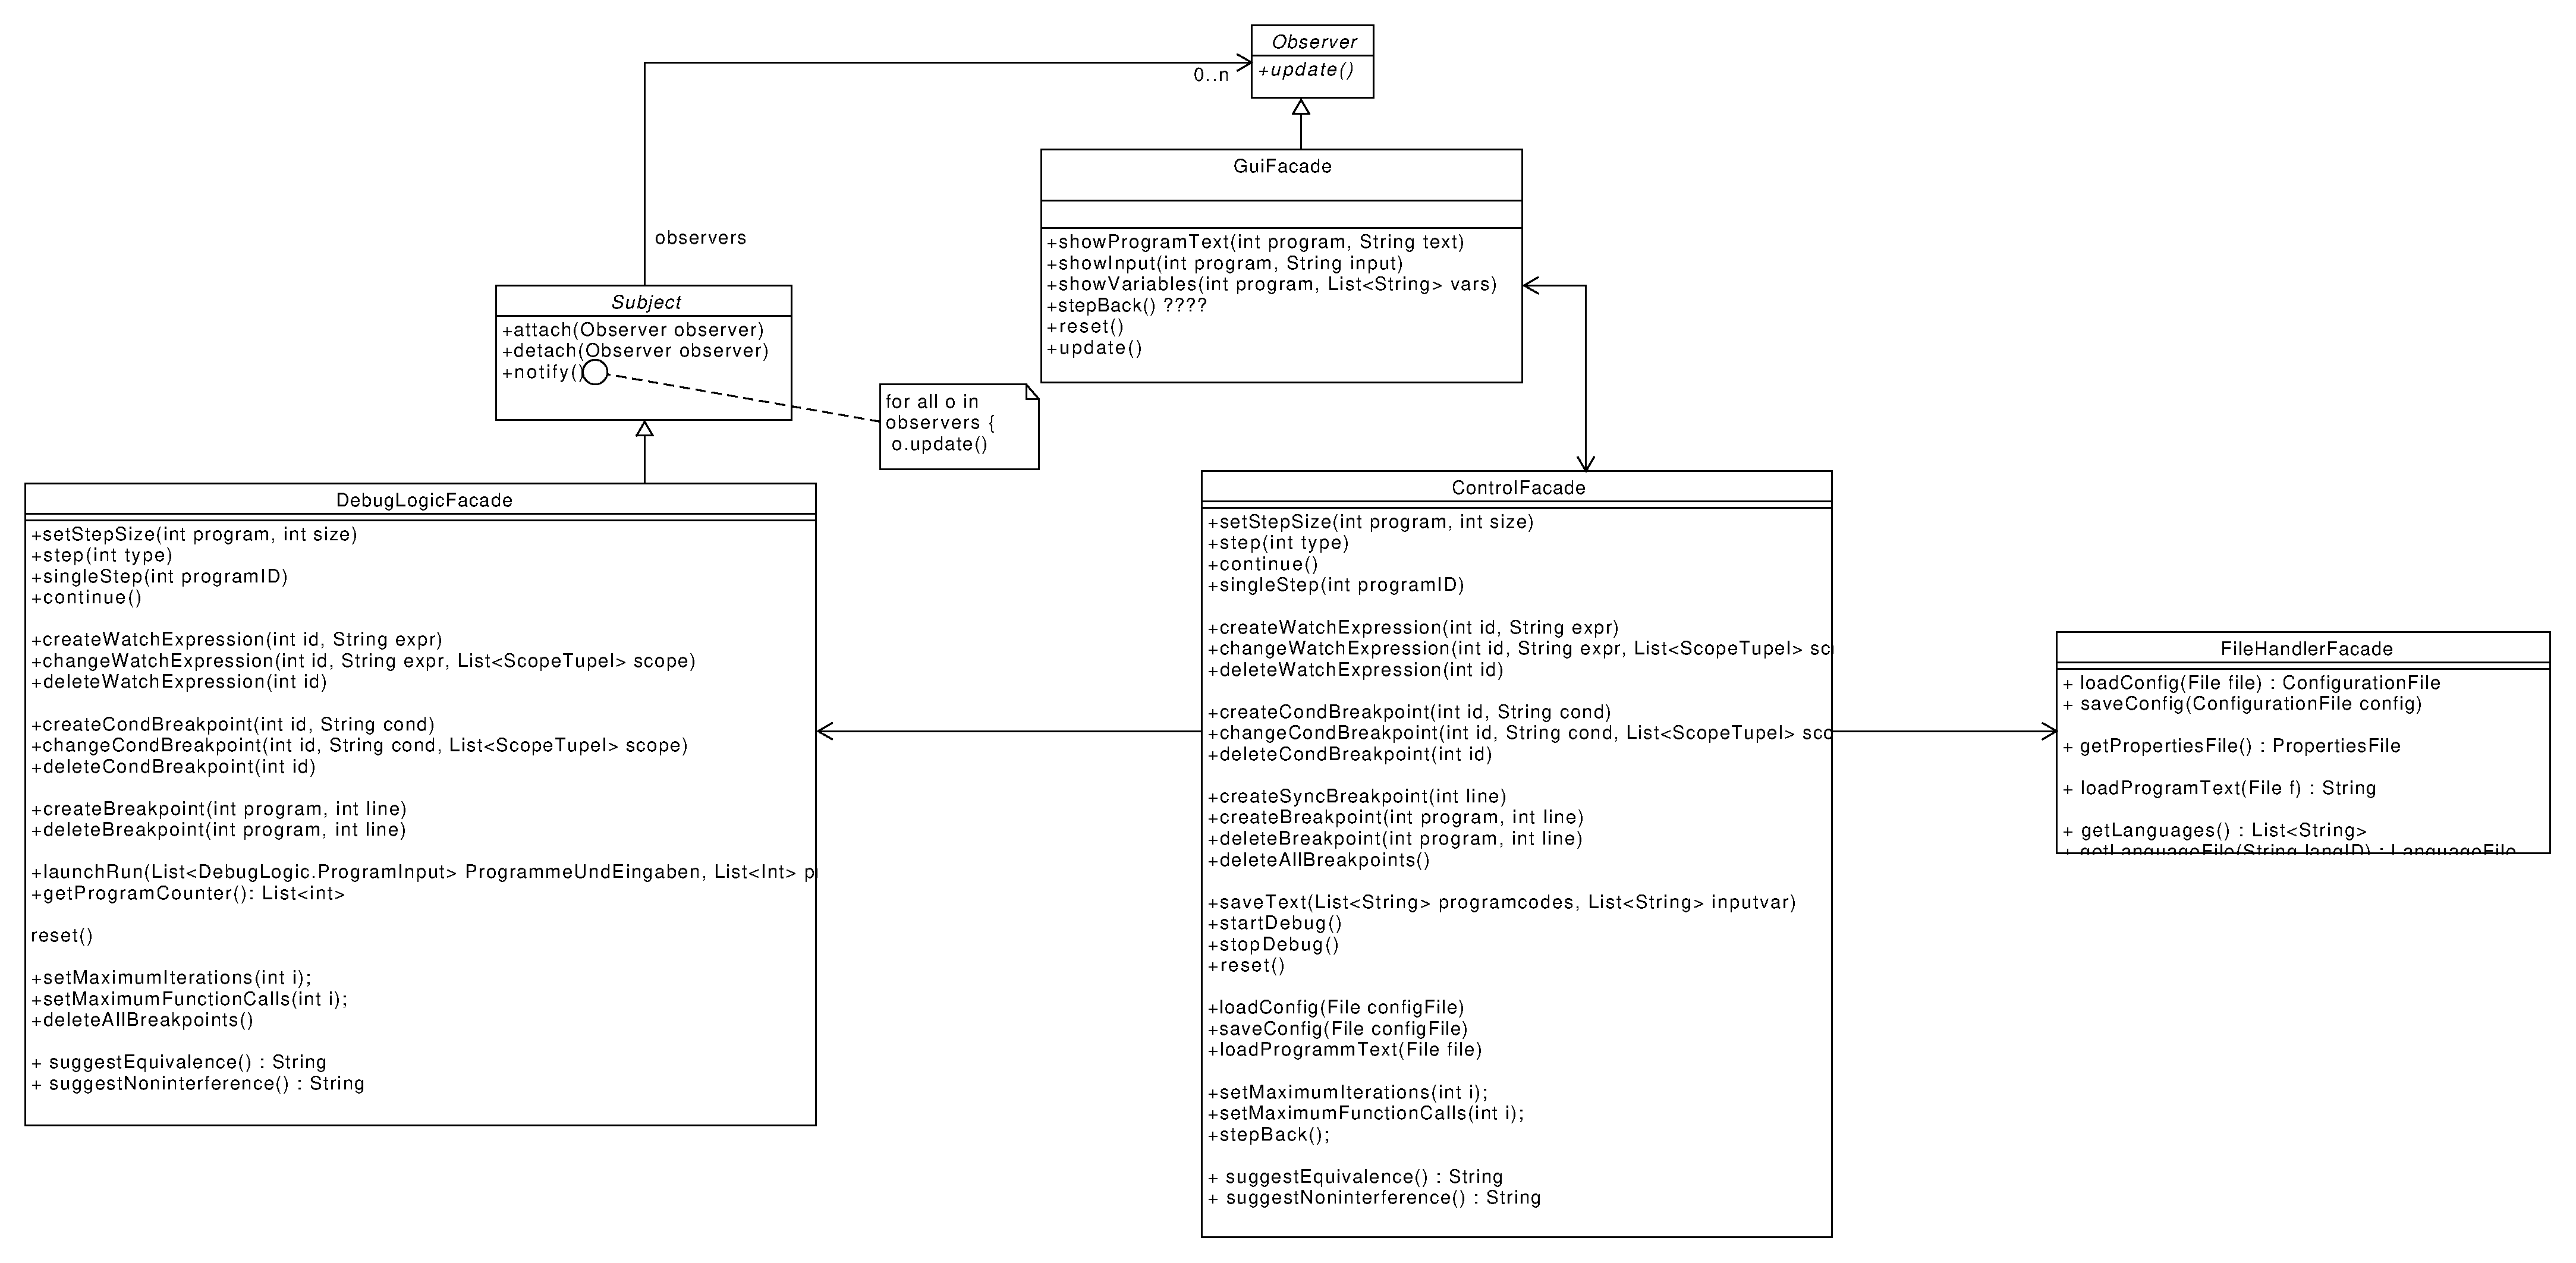
\includegraphics[width=0.8\textwidth]{diagrammIdeenUmlet/fassaden.pdf}
\caption{Die Schnittstellen der Pakete durch Fassaden dargestellt}
\label{Terme}
\end{figure}
\paragraph{Das Observerpattern im MVC}
Im Rahmen einer MVC-Architektur, ist es notwendig, dass die Viewkomponente eine Zustandsänderung des Modells sofort erfährt und darauf reagieren kann, indem sie sich die von ihr zur Anzeige benötigten Daten holt. Da es der Erweiterbarkeit wegen auch möglich sein soll, einmal mehrere verschiedene dieser beobachtenden Viewkomponenten ein Modell beobachten zu lassen, empfiehlt sich das Entwurfsmuster \enquote{Observer}. Die von diesem Pattern zur Verfügung gestellte 1-zu-n Abhängigkeit passt damit hervorragend zur vorliegenden Problemstellung: Aus Gründen der Wiederverwendbarkeit darf das Modell nicht festsetzen, welche und wie viele solcher Beobachter es hat. Die allgemein definierten Schnittstellen \textit{Observer} und \textit{Subject} ermöglichen dies. 
\paragraph{Das Fassadenpattern}
Durch die Einteilung des Systems in einzelne Subsysteme in Form von Paketen, ist es von Nöten, Schnittstellen dieser Subsysteme zu definieren. Diese sollten fest sein und sich bei Änderung der internen Struktur eines Subsystems nicht ändern, sodass das Geheimnisprinzip eingehalten wird. Um zusätzlich die Abhängigkeiten der Pakete zwischeneinander im Sinne einer losen Kopplung gering zu halten, bietet sich das Entwurfsmuster \enquote{Facade} an. Jegliche Kommunikation zwischen den in \ref{Packages} beschriebenen Paketen findet also über Fassaden statt. Das ermöglicht, die Schnittstellen des Paketes an einer Stelle zu definieren, und festgelegte Eintrittspunkte für die Kommunikation zwischen den Paketen zu bieten.
\subsection{Patterns im Paket User Interface}
Durch die Nutzung von Swing besteht der Grundaufbau des User Interfaces aus einem \enquote{Kompositum}. 
Durch anonyme Instanzen von Action Listenern wird das Befehlsmuster implementiert. \\
Des Weiteren werden die Entwurfsmuster Vererbung (z.B. DebuggerPopUp und ErrorPopUp) und Beobachter (durch das MVC-Konzept vorgegeben) in den Klassen ExpressionPanel und ProgramPanel implementiert.
Die Klassen CondBreakpointPanel und WatchExpressionPanel stellen Singletons dar. %TODO eventuell Erklären welche vorteile das ergibt
\subsection{Patterns im Paket Control}
Die Kontrollkomponente muss, je nachdem ob sich die Anwendung (DIbugger) im Debug- 
oder Editiermodus befindet, bestimmte Änderungen am Modell zulassen (bei Anfragen
zwischen Modell und Präsentation vermitteln), oder sie verwähren (nicht vermitteln)\\.
Da während der Laufzeit der Anwendung zwischen beiden Modi gewechselt werden kann,
bietet sich hier das Zustandsmuster an.\\
Die Control-Implementation wird durch entfallende eingebettete Zustandsspeicherung
in Form von redundanten Abfragen in den Methoden der Fassade leichter wartbar und
die Entkopplung des Systems wird gefördert. 
\subsection{Patterns im Paket Debug Logic}
\paragraph{Die Strategie für Vorschlagsgenerierung}
Ein Teil des Subpaketes \textit{DebugLogic.Debugger} ist verantwortlich für die Erzeugung von Vorschlägen für Nutzereingaben, Watch-Expressions und bedingten Breakpoints oder Schrittgrößen. Da man das Verfahren, einen solchen Vorschlag zu generieren, beliebig komplex gestalten kann, sollen die verwendeten Algorithmen austauschbar und variabel gehalten werden. Dafür bietet sich das Entwurfsmuster \enquote{Strategie} besonders an. Im Entwurf wird es durch die Interfaces \textit{StepSizeSuggestion, RelationalSuggestion} und InputValueSuggestion realisiert.
\paragraph{Das Kompositum}
Das Entwurfsmuster \enquote{Kompositum} wird im Paket \textit{DebugLogic.Interpreter} ausgiebig verwendet. Aufgrund der in Programmiersprachen gegebenen Strukturen wie zum Beispiel Termen, die sich durch Baumstrukturen sowohl abbilden als auch einfach rekursiv auswerten lassen, empfiehlt sich dieses Pattern. Die inhärente Struktur solcher rekursiv definierbarer Strukture wird von einem \enquote{Kompositum} perfekt repräsentiert. Das Muster ermöglicht dabei den Nutzern der entsprechenden Klassen einen einheitlichen Umgang mit einzelnen und zusammengesetzten Objekten.
\begin{figure}[!h]
\centering
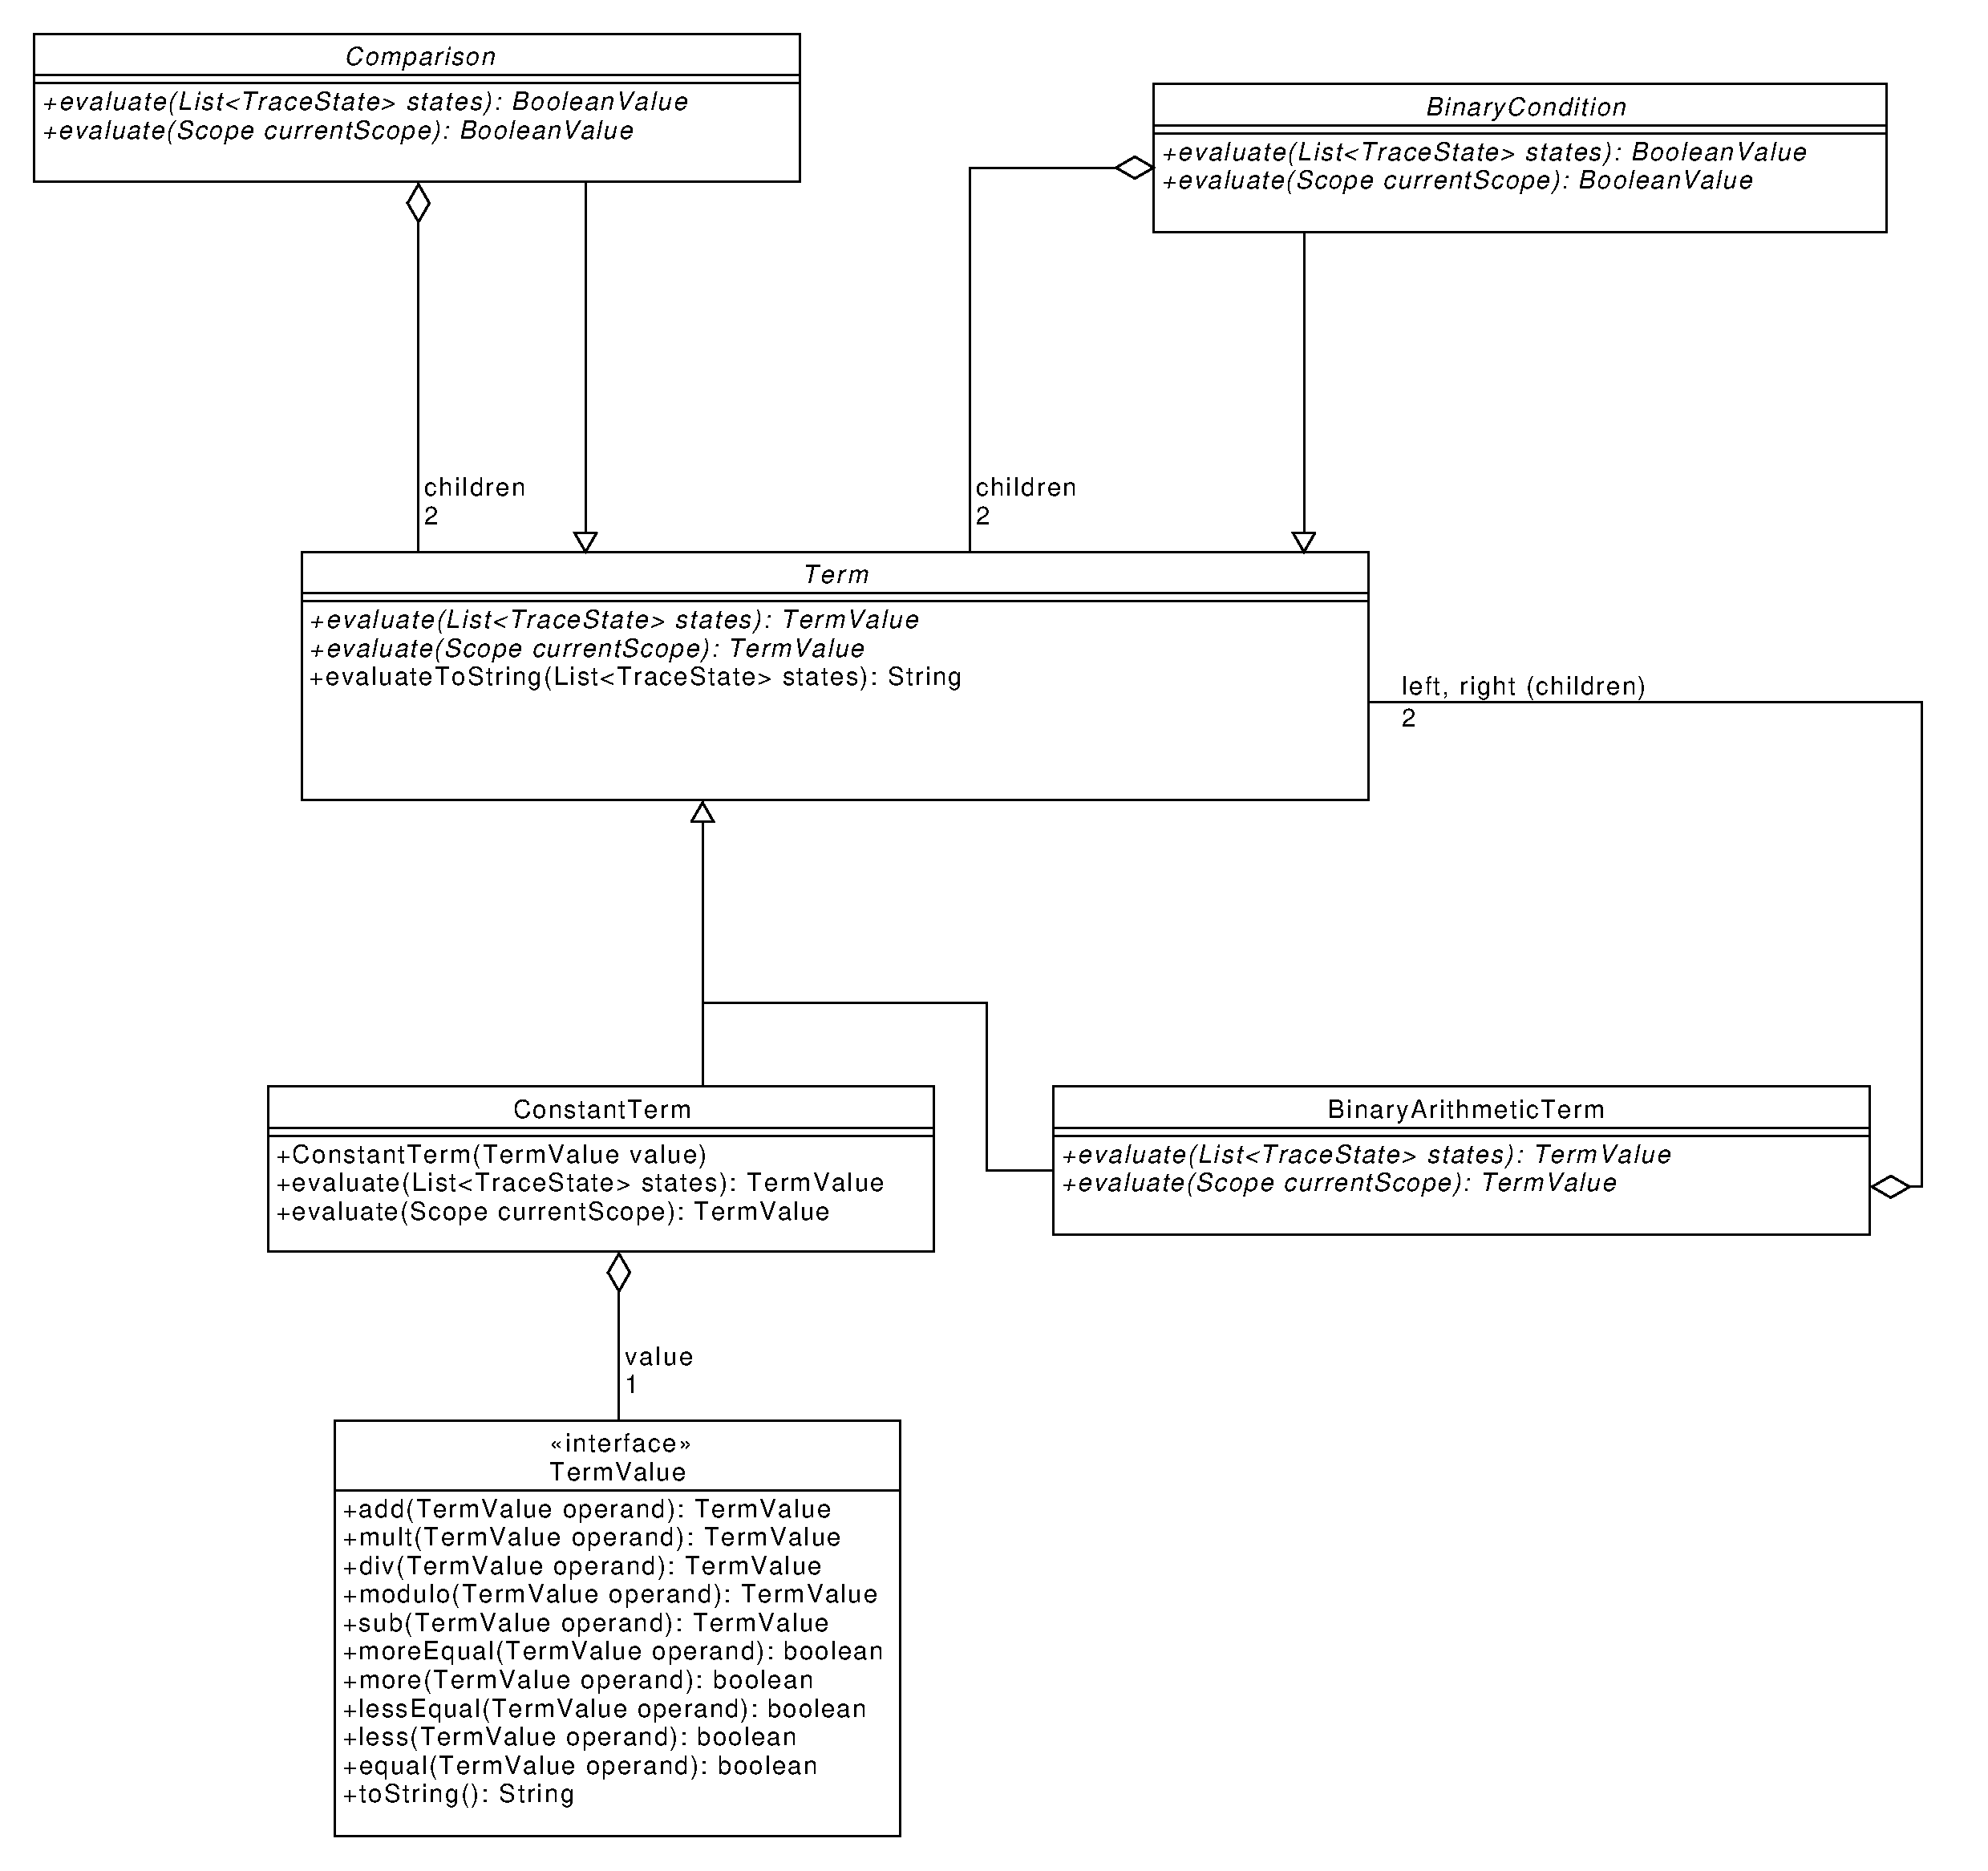
\includegraphics[width=0.8\textwidth]{diagrammIdeenUmlet/TermCondition.pdf}
\caption{Das Termkompositum im Entwurf}
\label{Terme}
\end{figure}
\begin{figure}[!h]
\centering
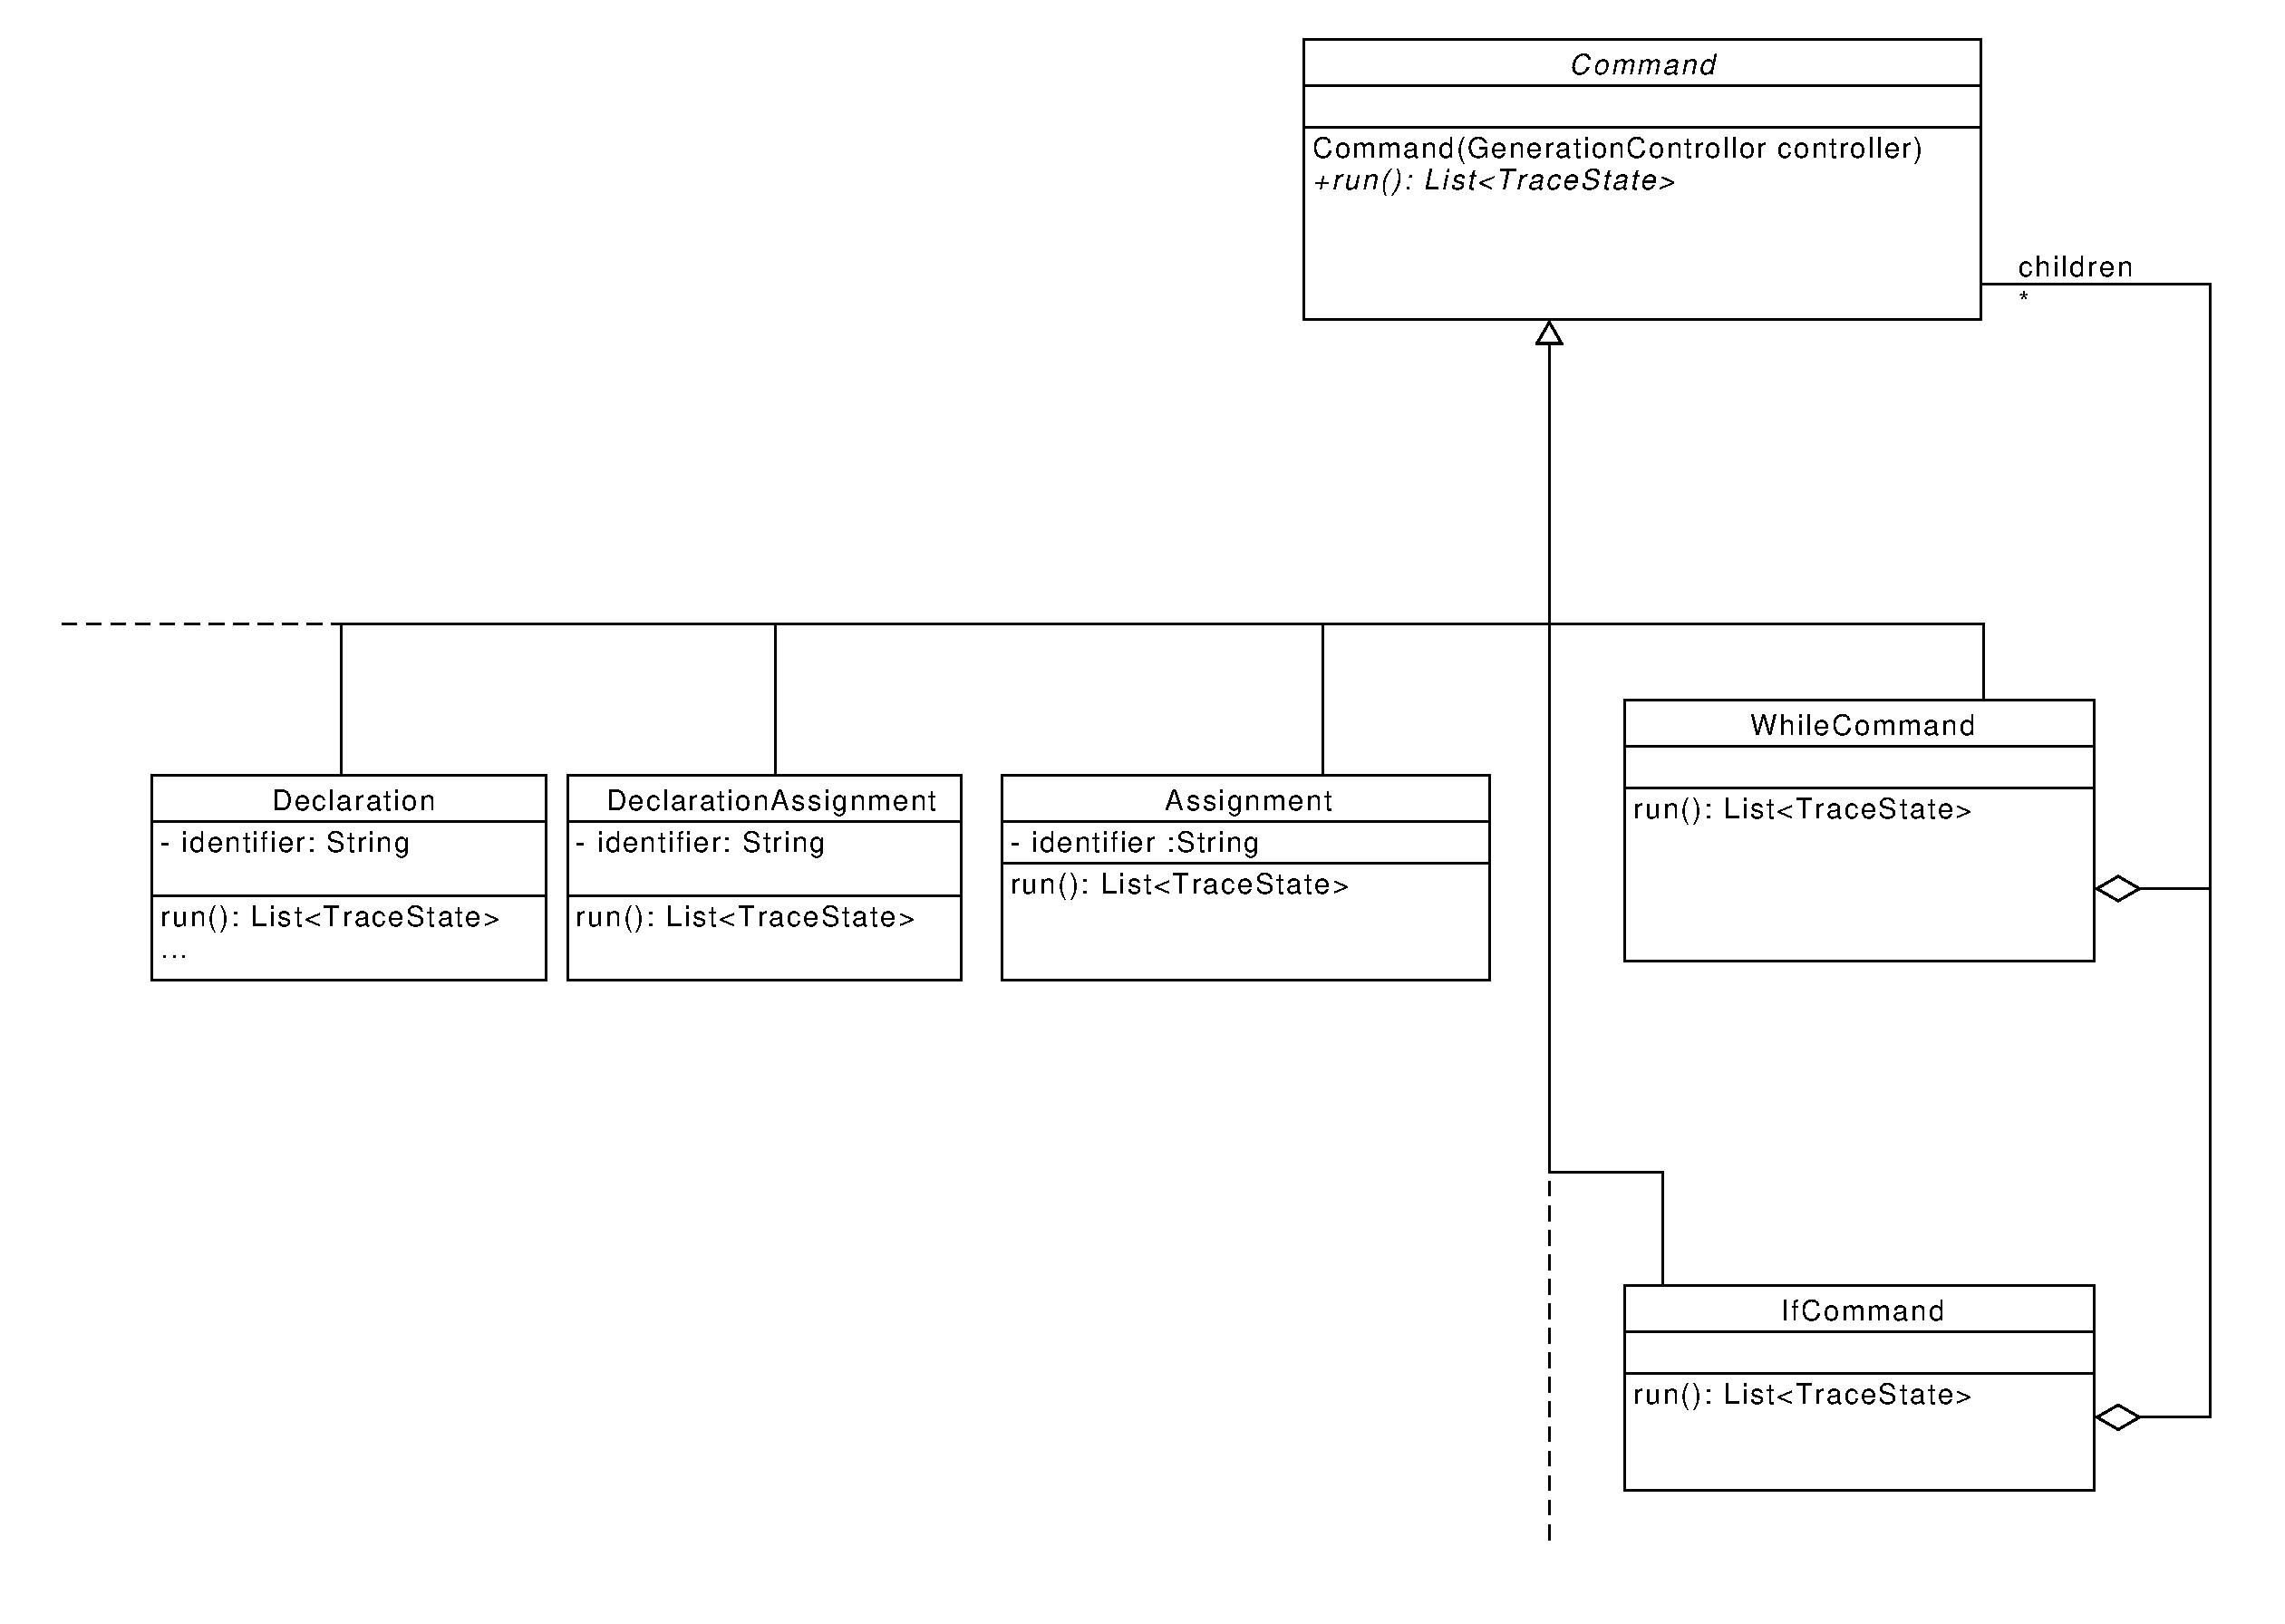
\includegraphics[width=0.8\textwidth]{diagrammIdeenUmlet/CommandComposite.pdf}
\caption{Die Klasse \textit{Command} als Kompositum}
\label{Command}
\end{figure}
\paragraph{Das Termkompositum}
Die Struktur eines Termes kann wie folgt beschrieben werden:
Konstanten und Variablen sind Terme. Sind $A$ und $B$ Terme und $\sigma$ ein zweistelliger Operator, dann ist auch $A\sigma B$ ein Term. Ist $\nabla$ ein einstelliger Operator, dann ist auch $\nabla A$ ein Term. Diese induktiv aufgebaute Struktur der Terme lässt sich in naheliegender Weise in eine Klassenstruktur übertragen, die in Abbildung \ref{Terme} dargestellt ist. Hier wird das Entwurfsmuster \enquote{Kompositum} verwendet. Der Vorteil besteht in der einfachen und einheitlichen Nutzung der Funktion \textit{evaluate()}. Diese gibt eine Instanz vom Typ \textit{TermValue} zurück. Die vollständige Funktionalität des vorliegenden Typsystems ist in den Implementierungen dieser Schnittstelle gekapselt. Einen Spezialfall von Termen stellen \textit{BinaryCondition} und \textit{Comparison} dar. Diese werten sich per Definition zu booleschen Werten aus. Das Liskovsche Substitutionsprinzip erlaubt Kovarianz in den Ausgabeparametern, weswegen es möglich ist, diesen Subklassen von \textit{Term} in den \textit{evaluate()}-Methoden den Rückgabetyp \textit{BooleanValue} zu geben, eine spezielle Implementierung des \textit{TermValue}-Interfaces.
\paragraph{Das Commandkompositum und Befehlsmuster}
Ein weiteres \enquote{Kompositum} wird für die Klasse \textit{Command} und ihre Subklassen verwendet. Ein Auszug davon ist in Abbildung \ref{Command} zu sehen. Zunächst gibt es elementare Befehle, wie etwa eine einfache Zuweisung. Es gibt jedoch auf Befehle, wie etwa while- und if- Befehle, die mehrere Unterbefehle haben, und entscheiden müssen, ob und wie oft diese ausgeführt werden. Sie stellen also in diesem Fall Befehlskompositionen dar. Ein großer Vorteil dieser Modellierung besteht in der Nutzung der Methode \textit{run()}. Der Aufrufer eines Befehls muss nicht wissen, ob es sich um einen elementaren Zuweisungs- oder Deklarationsbefehl oder um einen komplexen zusammengesetzten Befehl wie etwa eine Schleife handelt. Ihn interessiert nur die während der Ausführung des Befehls angenommenen Zustände. Die Befehlsfunktionalität wird so weggekapselt. \\
Einen Befehl als Objekt zu kapseln, um diesen in Warteschlangen zu fügen, aufzubewahren oder Empfänger damit zu parametrisieren ist der Zweck des Entwurfsmusters \enquote{Command}, das hier auch verwendet ist. Da die Befehle zunächst alle erzeugt und dann später ausgeführt werden. Die Ausführung der Befehle ist entsprechend komplex, da dabei etwa Typprüfungen stattfinden müssen (Näheres dazu ist in Kapitel \ref{charAbl} zu finden), weswegen es sich auch empfiehlt diese Arbeit zu kapseln. 
\paragraph{Das Visitorpattern}
Um die Term- und Befehlsstrukturen zu erzeugen, wird im Entwurf das Entwurfsmuster \textit{Visitor} verwendet. Zum einen ermöglicht es, die von Antlr generierten \textit{ParseTree}-Objekte mit den von Antlr vorgegebenen Schnittstellen zu durchlaufen. Zum anderen bietet dieses Pattern die Möglichkeit, beliebige Operationen auf den Ableitungsbäumen auszuführen, ohne die von Antlr generierten Klassenstrukturen zu verändern. Die Nutzung dieses Patterns ist daher beim Umgang mit Antlr beinahe unumgänglich.
\paragraph{Der Traceiterator}
\begin{figure}[!h]
\centering
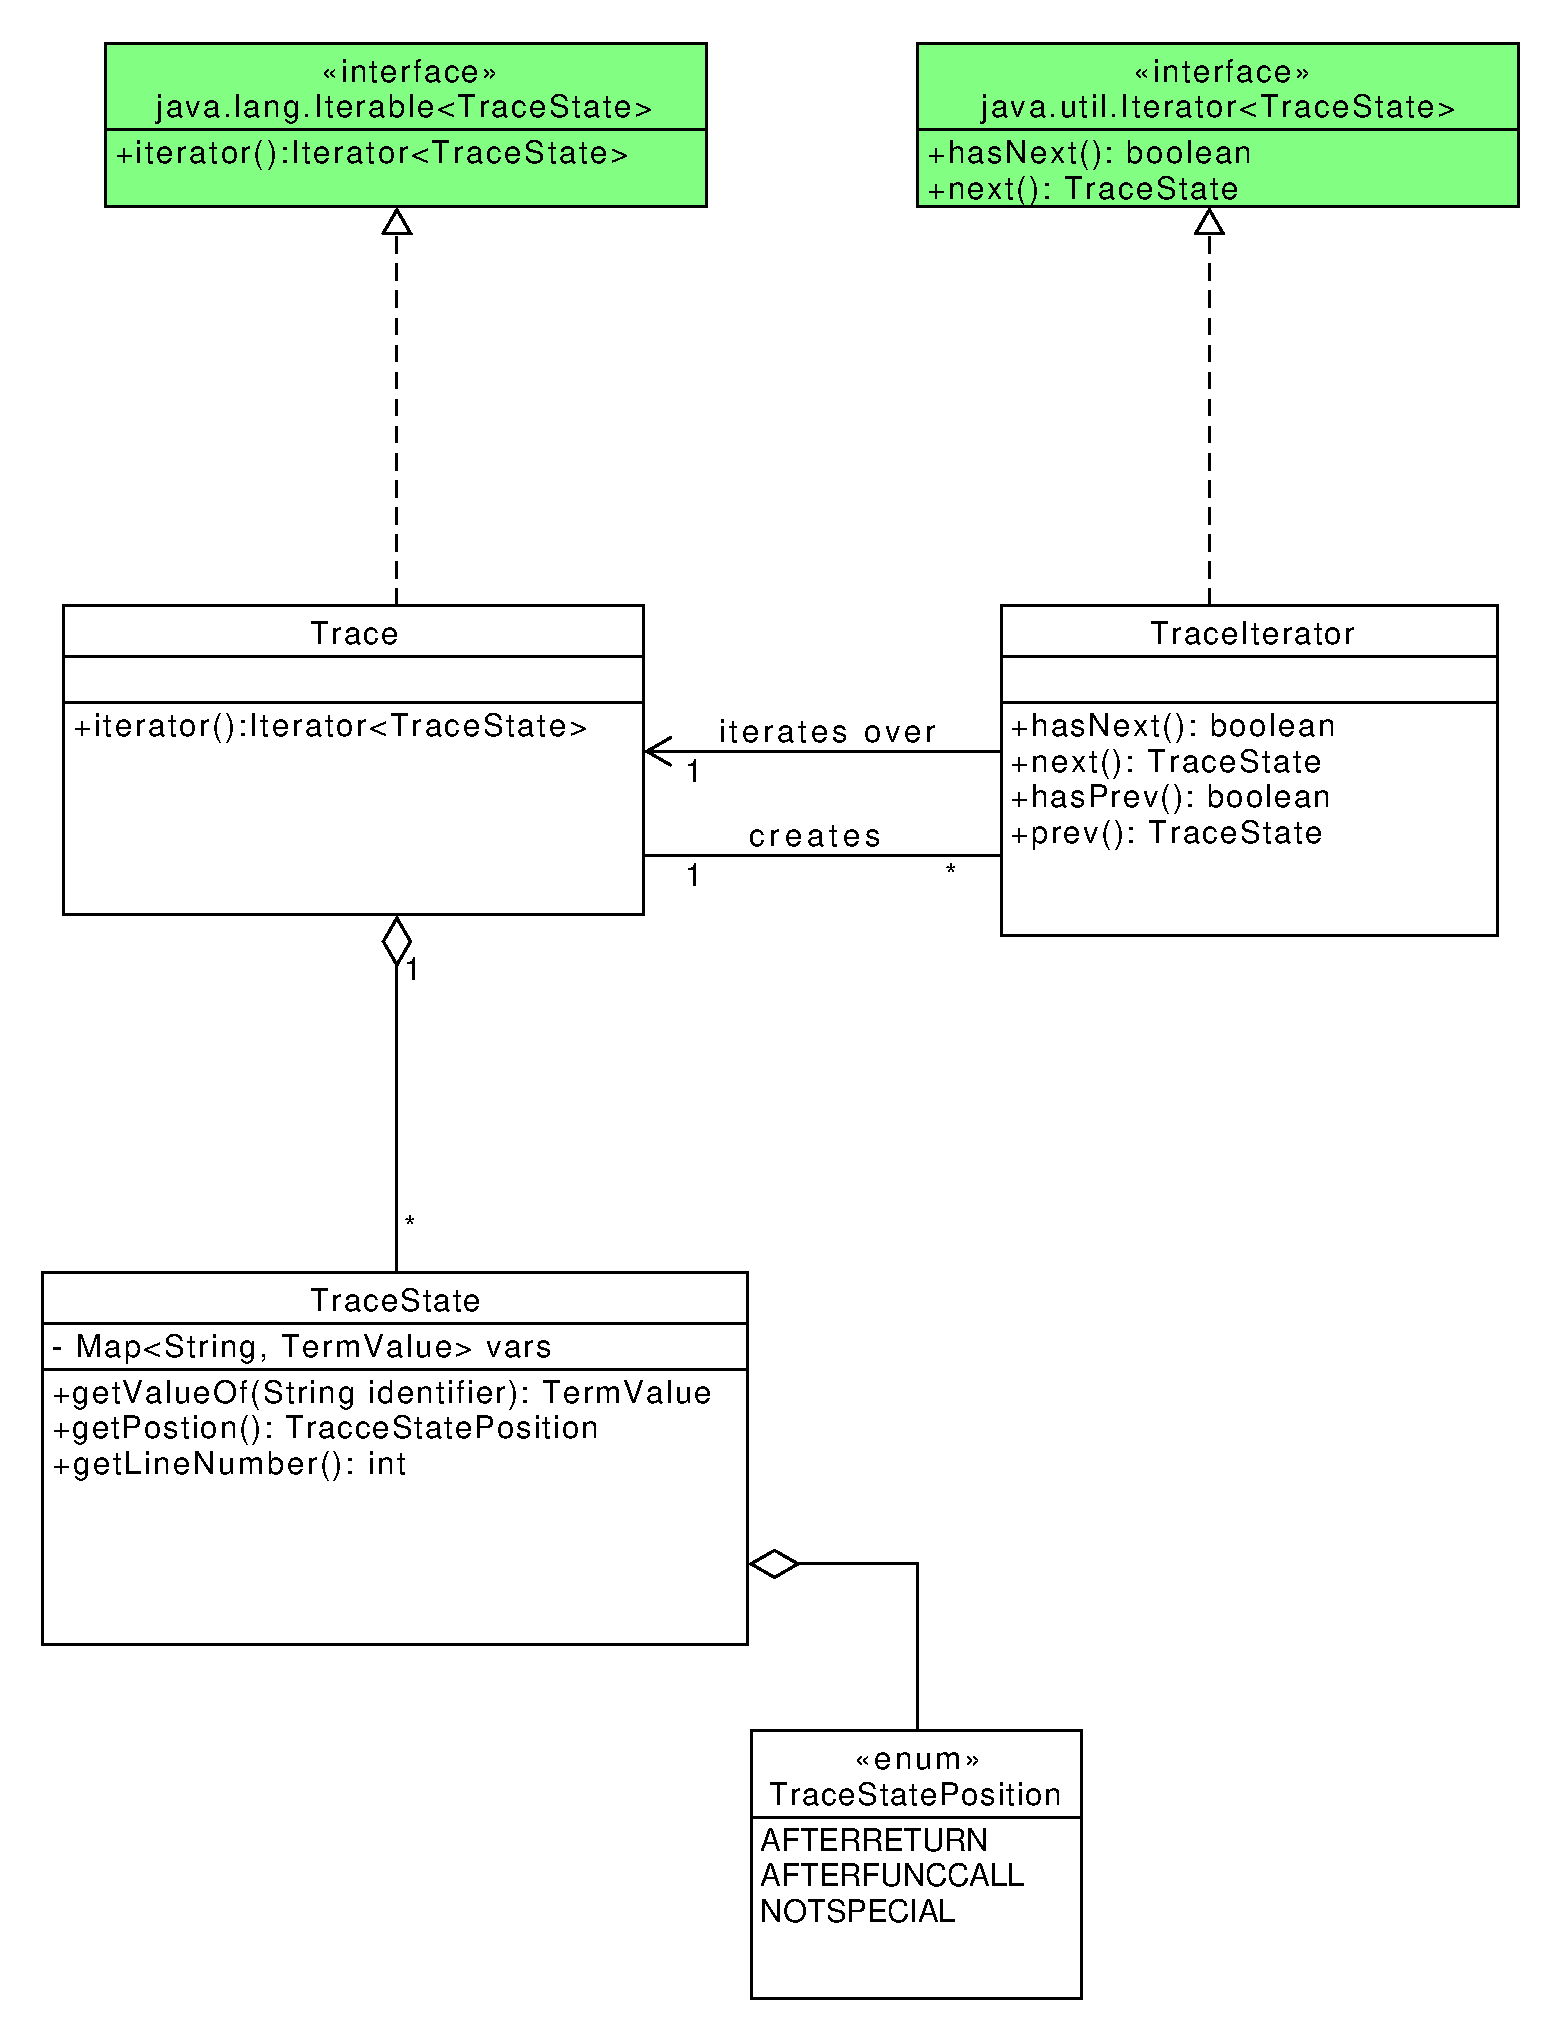
\includegraphics[width=0.8\textwidth]{diagrammIdeenUmlet/TraceIteratorPattern.pdf}
\caption{Der Traceiterator}
\label{TraceIterator}
\end{figure}
Wir betrachten Abbildung \ref{TraceIterator}.
Grundkonzept des Debuggens ist die folgende Idee: Zunächst wird die komplette Ausführung eines Programmlaufes berechnet und dabei nach jedem ausgeführten Befehl der Zustand der Variablen gespeichert. Die Aggregation all dieser als \textit{TraceState}-Instanzen dargestellten Zustände ist ein sogenanntes \textit{Trace}-Objekt. Um es dem Paket \textit{DebugLogic.Debugger} zu ermöglichen, ohne Kenntnis der konkreten Darstellung dieses Traces über die \textit{TraceState}-Objekte zu iterieren, wird lediglich ein \textit{TraceIterator}-Objekt nach aussen gegeben. Um dabei die volle von Java angebotene Funktionalität zu nutzen, werden die entsprechenden Java Schnittstellen implementiert. 
\subsection{Patterns im Paket File Handler}
Das Paket FileHandler.Facade stellt vier abstrakte Klassen zum Lesen und Schreiben von Sprach-, Einstellungs- und Konfigurationsdateien bereit. Dadurch wird das \enquote{Strategie}-Muster implementiert und vom Paket FileHandler.RDBF genutzt. Dabei wird für jede Abstrakte Klasse eine spezielle Strategie zur Verfügung gestellt. Jedoch können später weitere zum Lesen und Schreiben von anderer Dateiformaten, z.B. XML, Json... , implementiert werden. Somit dient die Verwendung des Musters vor allem der Erweiterbarkeit.\\
Das Entwurfsmuster Einzelstück (Singleton) wurde bei der Klasse RDBFParser verwendet, da diese keine Daten speichern muss und nur für das Lesen und richtige Interpretieren von Zeilen verantwortlich ist. So wird  ein globaler Zugriffspunkt bereitgestellt und es wird sichergestellt, dass stets nur ein Parser exisitiert.

\newpage
\section{Charakteristische Abläufe}\label{charAbl}
In diesem Kapitel werden charakteristische Abläufe des Produkts, wie der erste Programmaufruf und die
Anwendungsfälle, anhand von Sequenzdiagrammen dargestellt und erklärt.
 %TODO Auf Klassen oder Pakete in Beschreibung aller Klassen verweisen

\subsection{Erster Programmaufruf}
\begin{figure}[!h]
\centering
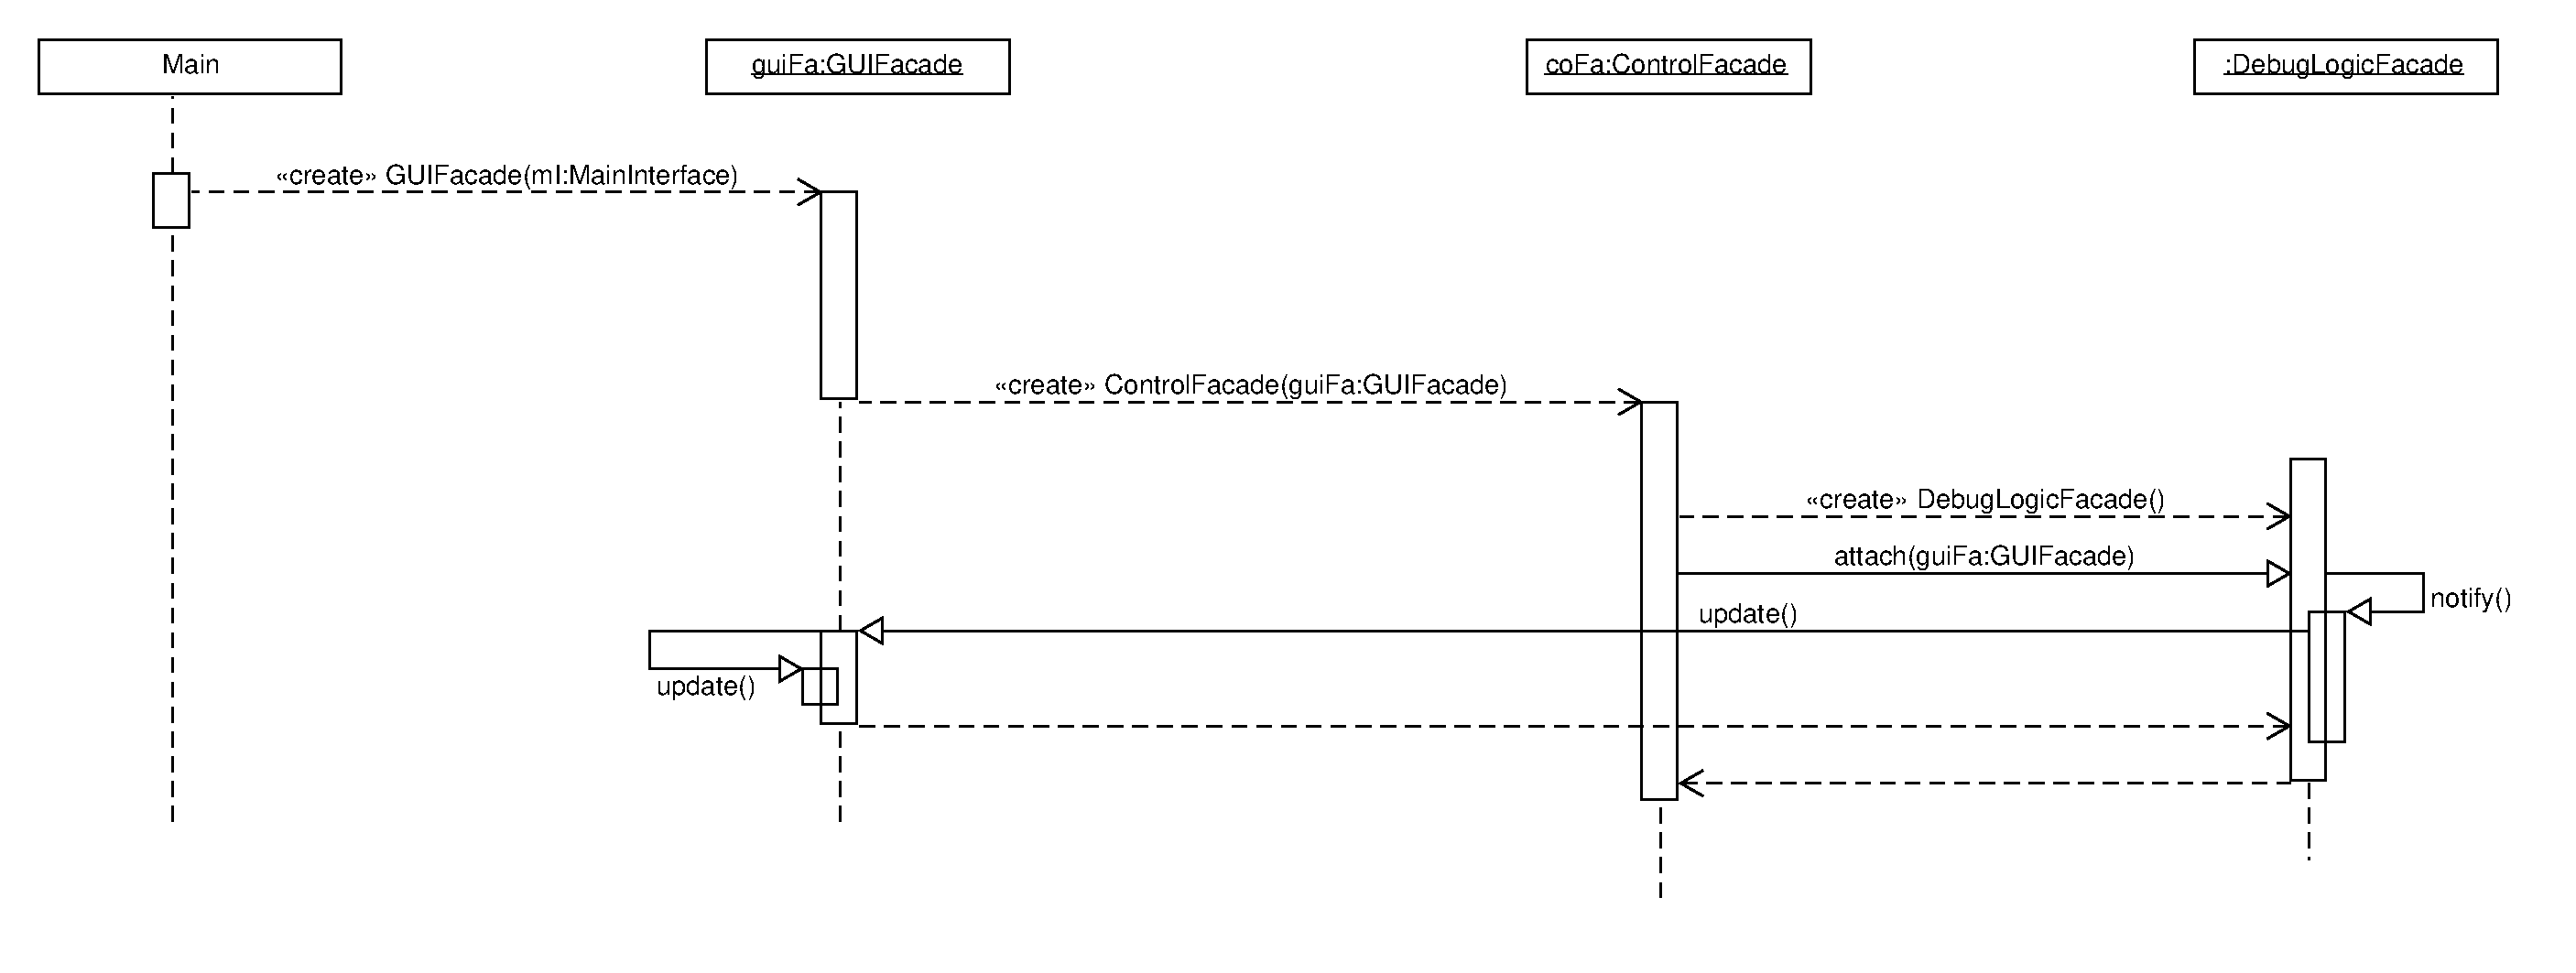
\includegraphics[width=0.8\textwidth]{diagrammIdeenUmlet/SequenceDiagrams/seq_firstCallPDF.pdf}
\caption{Sequenzdiagramm: Erster Programmaufruf}
\end{figure}
Wird das Produkt gestartet, erstellt die Main-Methode des MainInterface die GUIFacade und übergibt sich selbt.
Die GUIFacade speichert das MainInterface und erstellt ihrerseits die ControlFacade, welche wiederum
die DebugLogicFacade erstellt.
Die ControlFacade und DebugLogicFacade erstellen intern Instanzen der Klassen ihrer Pakete. \\
Die GUIFacade wird bei diesem Prozess bis zur DebugLogic weitergereicht, um dort als Observer angemeldet werden
zu können. Wird später dann zum Beispiel ein Breakpoint hinzugefügt, wird die GUIFacade benachrichtigt und
kann sich updaten.

\newpage
\subsection{Konfigurationsdatei laden}
\begin{figure}[!h]
\centering
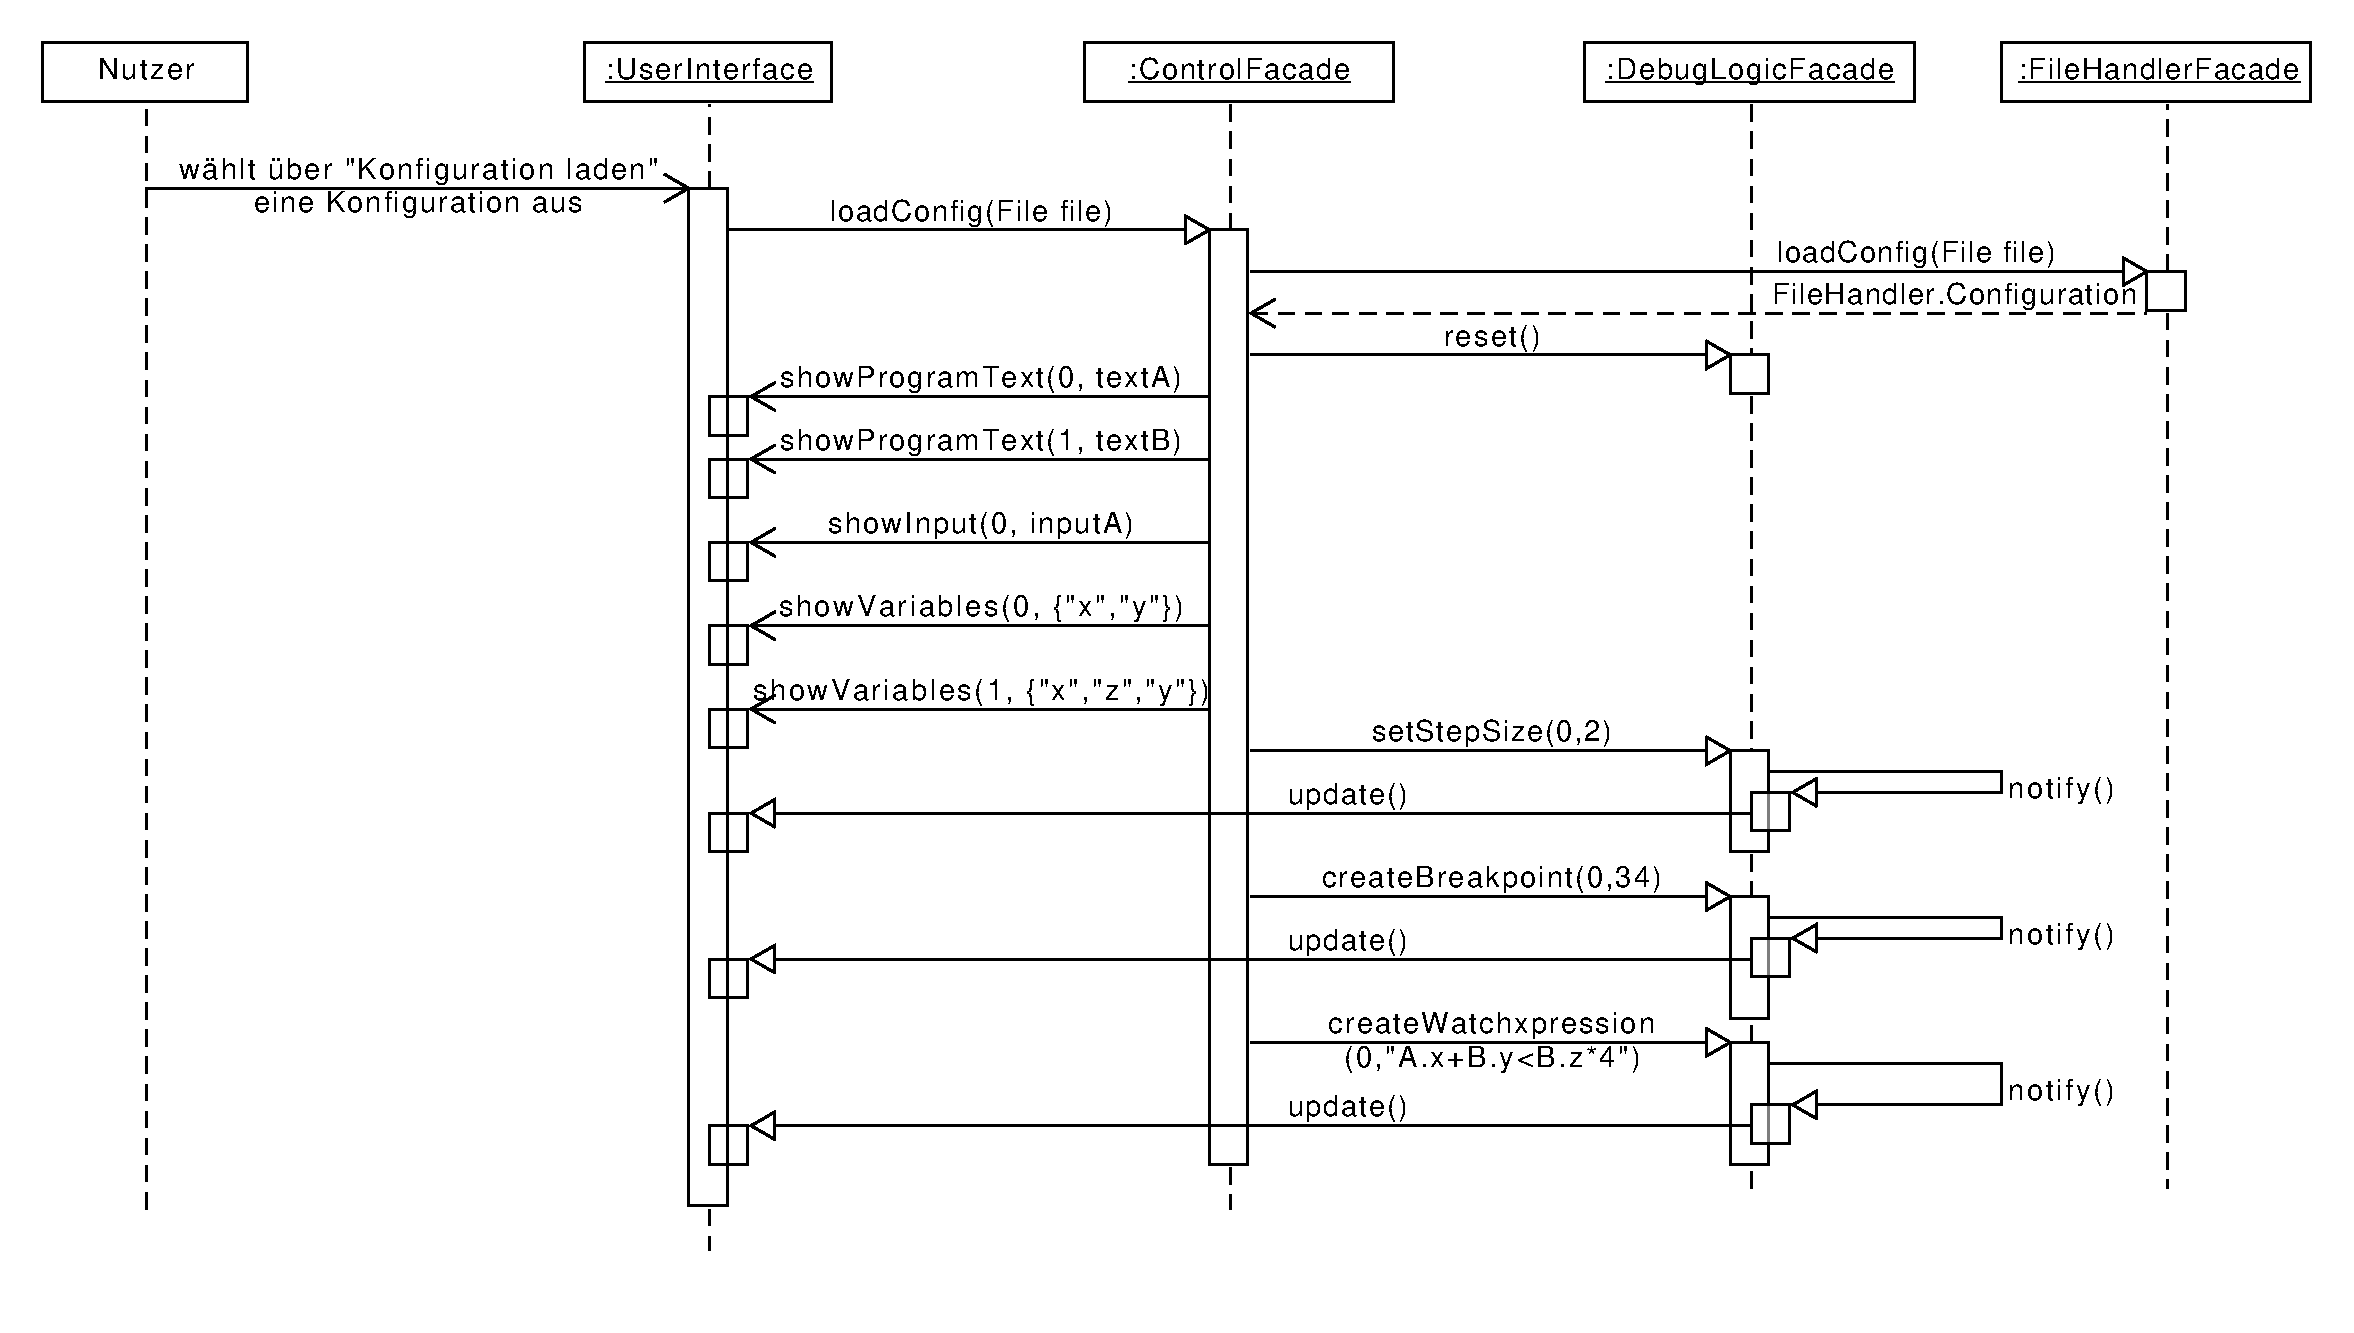
\includegraphics[width=0.8\textwidth]{diagrammIdeenUmlet/SequenceDiagrams/seq_loadConfigPDF.pdf}
\caption{Sequenzdiagramm:  Laden einer Konfigurationsdatei}
\end{figure}
Wählt der Benutzer über den Menpeintrag \enquote{Konfigurationsdatei laden} eine Konfiguration aus,
gibt das UserInterface diesen Befehl an die Control weiter, welche ein Configuration Objekt vom FileHandler 
erhält. \\
Die Control ruft anschließend Methoden der GUIFacade auf, um die Programmtexte, Eingabevariablen und
die im Variableninspektor anzuzeigende Variablen anzuzeigen. Außerdem ruft die Control
Mathoden der DebugLogicFacade auf, um für jedes Programm die Breakpoints, Watch-Expressions und
Schrittgrößen festzulegen. Über diese Änderungen wird das UserInterface als Observer benachrichtigt und
kann diese ebenfalls anzeigen

\newpage
\subsection{Konfigurationsdatei speichern}
\begin{figure}[!h]
\centering
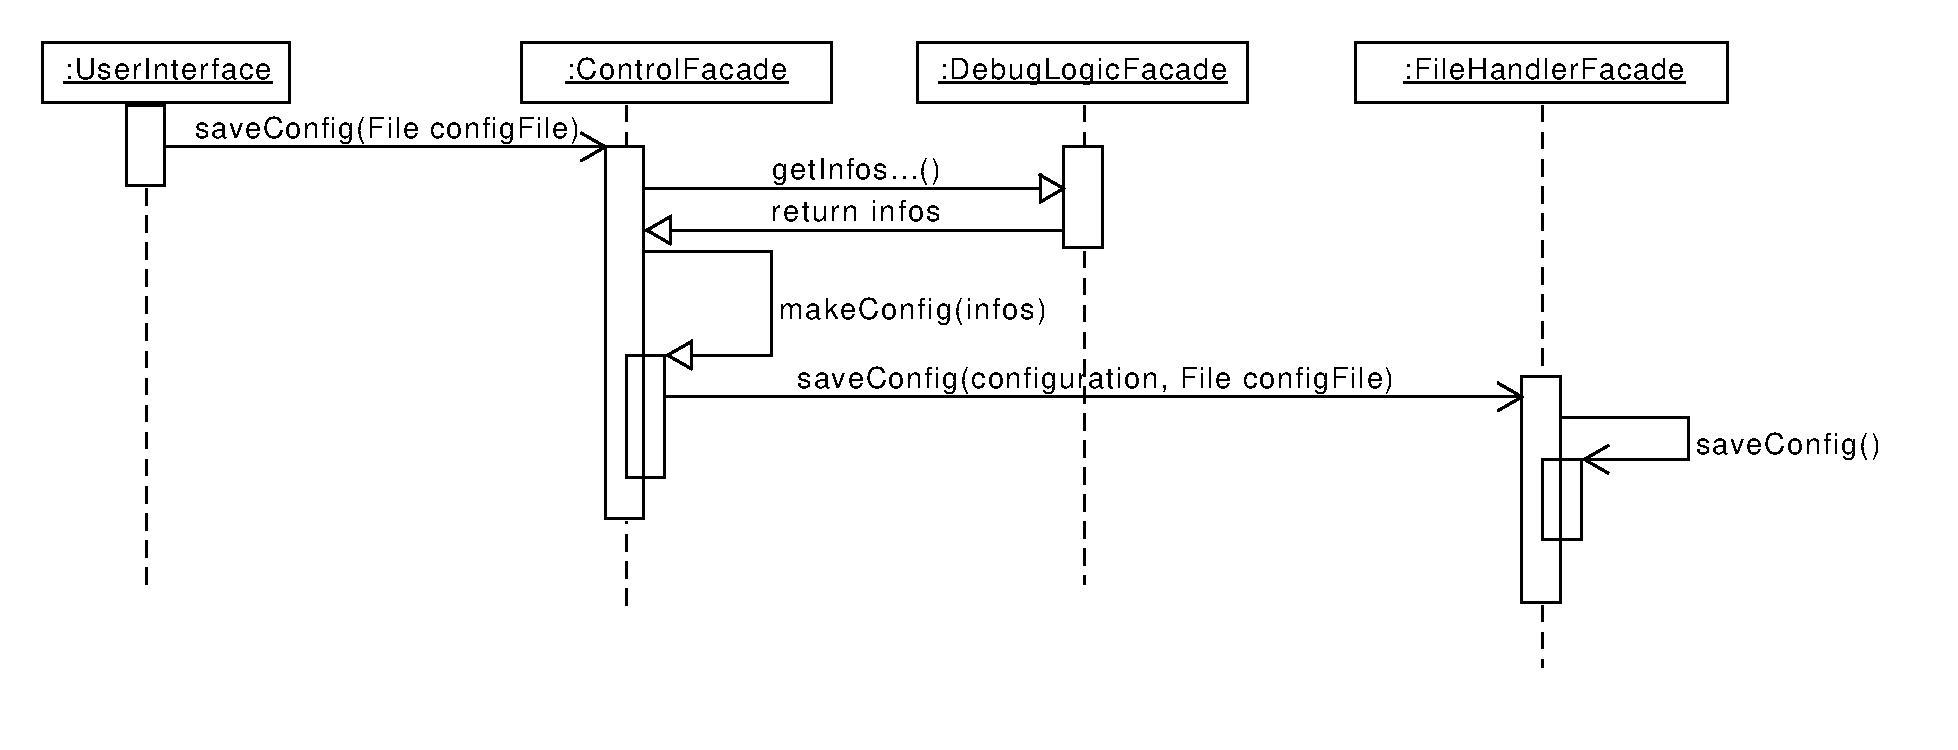
\includegraphics[width=0.8\textwidth]{diagrammIdeenUmlet/SequenceDiagrams/seq_saveConfigPDF.pdf}
\caption{Sequenzdigramm: Speichern einer Konfigurationsdatei}
\end{figure}
Möchte der Benutzer eine Konfigurationsdatei speichern, reicht das UserInterface den Speicherort
an die ControlFacade weiter. Die Control sammelt die benötigten Daten in einer Configuration Instanz.
Dieses Objekt wird mit dem angegebenen Speicherort an die FileHandlerFacade weitergegeben, welche 
dann die Konfigurationsdatei auf dem Rechner des Benutzers speichert.

\newpage
\subsection{AF10: Hinzufügen von Programmen}
\begin{figure}[!h]
\centering
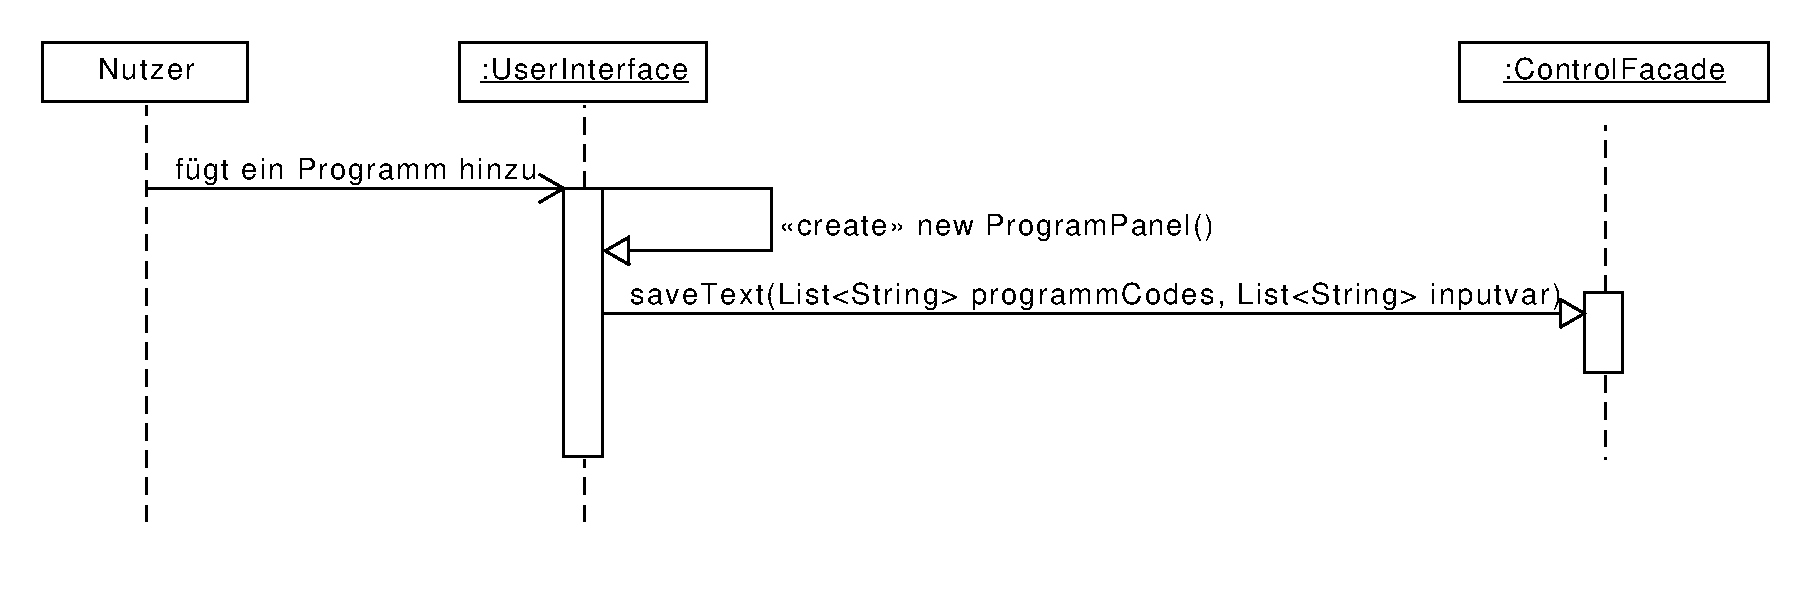
\includegraphics[width=0.8\textwidth]{diagrammIdeenUmlet/SequenceDiagrams/seq_AF10PDF.pdf}
\caption{Sequenzdiagramm: Hinzufügen von Programmen}
\end{figure}
Fügt der Benutzer über den Menüeintrag ein neues Programm hinzu, erstellt das UserInterface ein
neues ProgramPanel. Nach jedem Einfügen und Ändern von Programmtext oder Eingabevariablen, gibt
das UserInterface diese Informationen an die Control weiter, welche sie zu Start des Debugmodus
an die DebugLogic weiter gibt.

\newpage
\subsection{AF20: Ändern von Programmen}
\begin{figure}[!h]
\centering
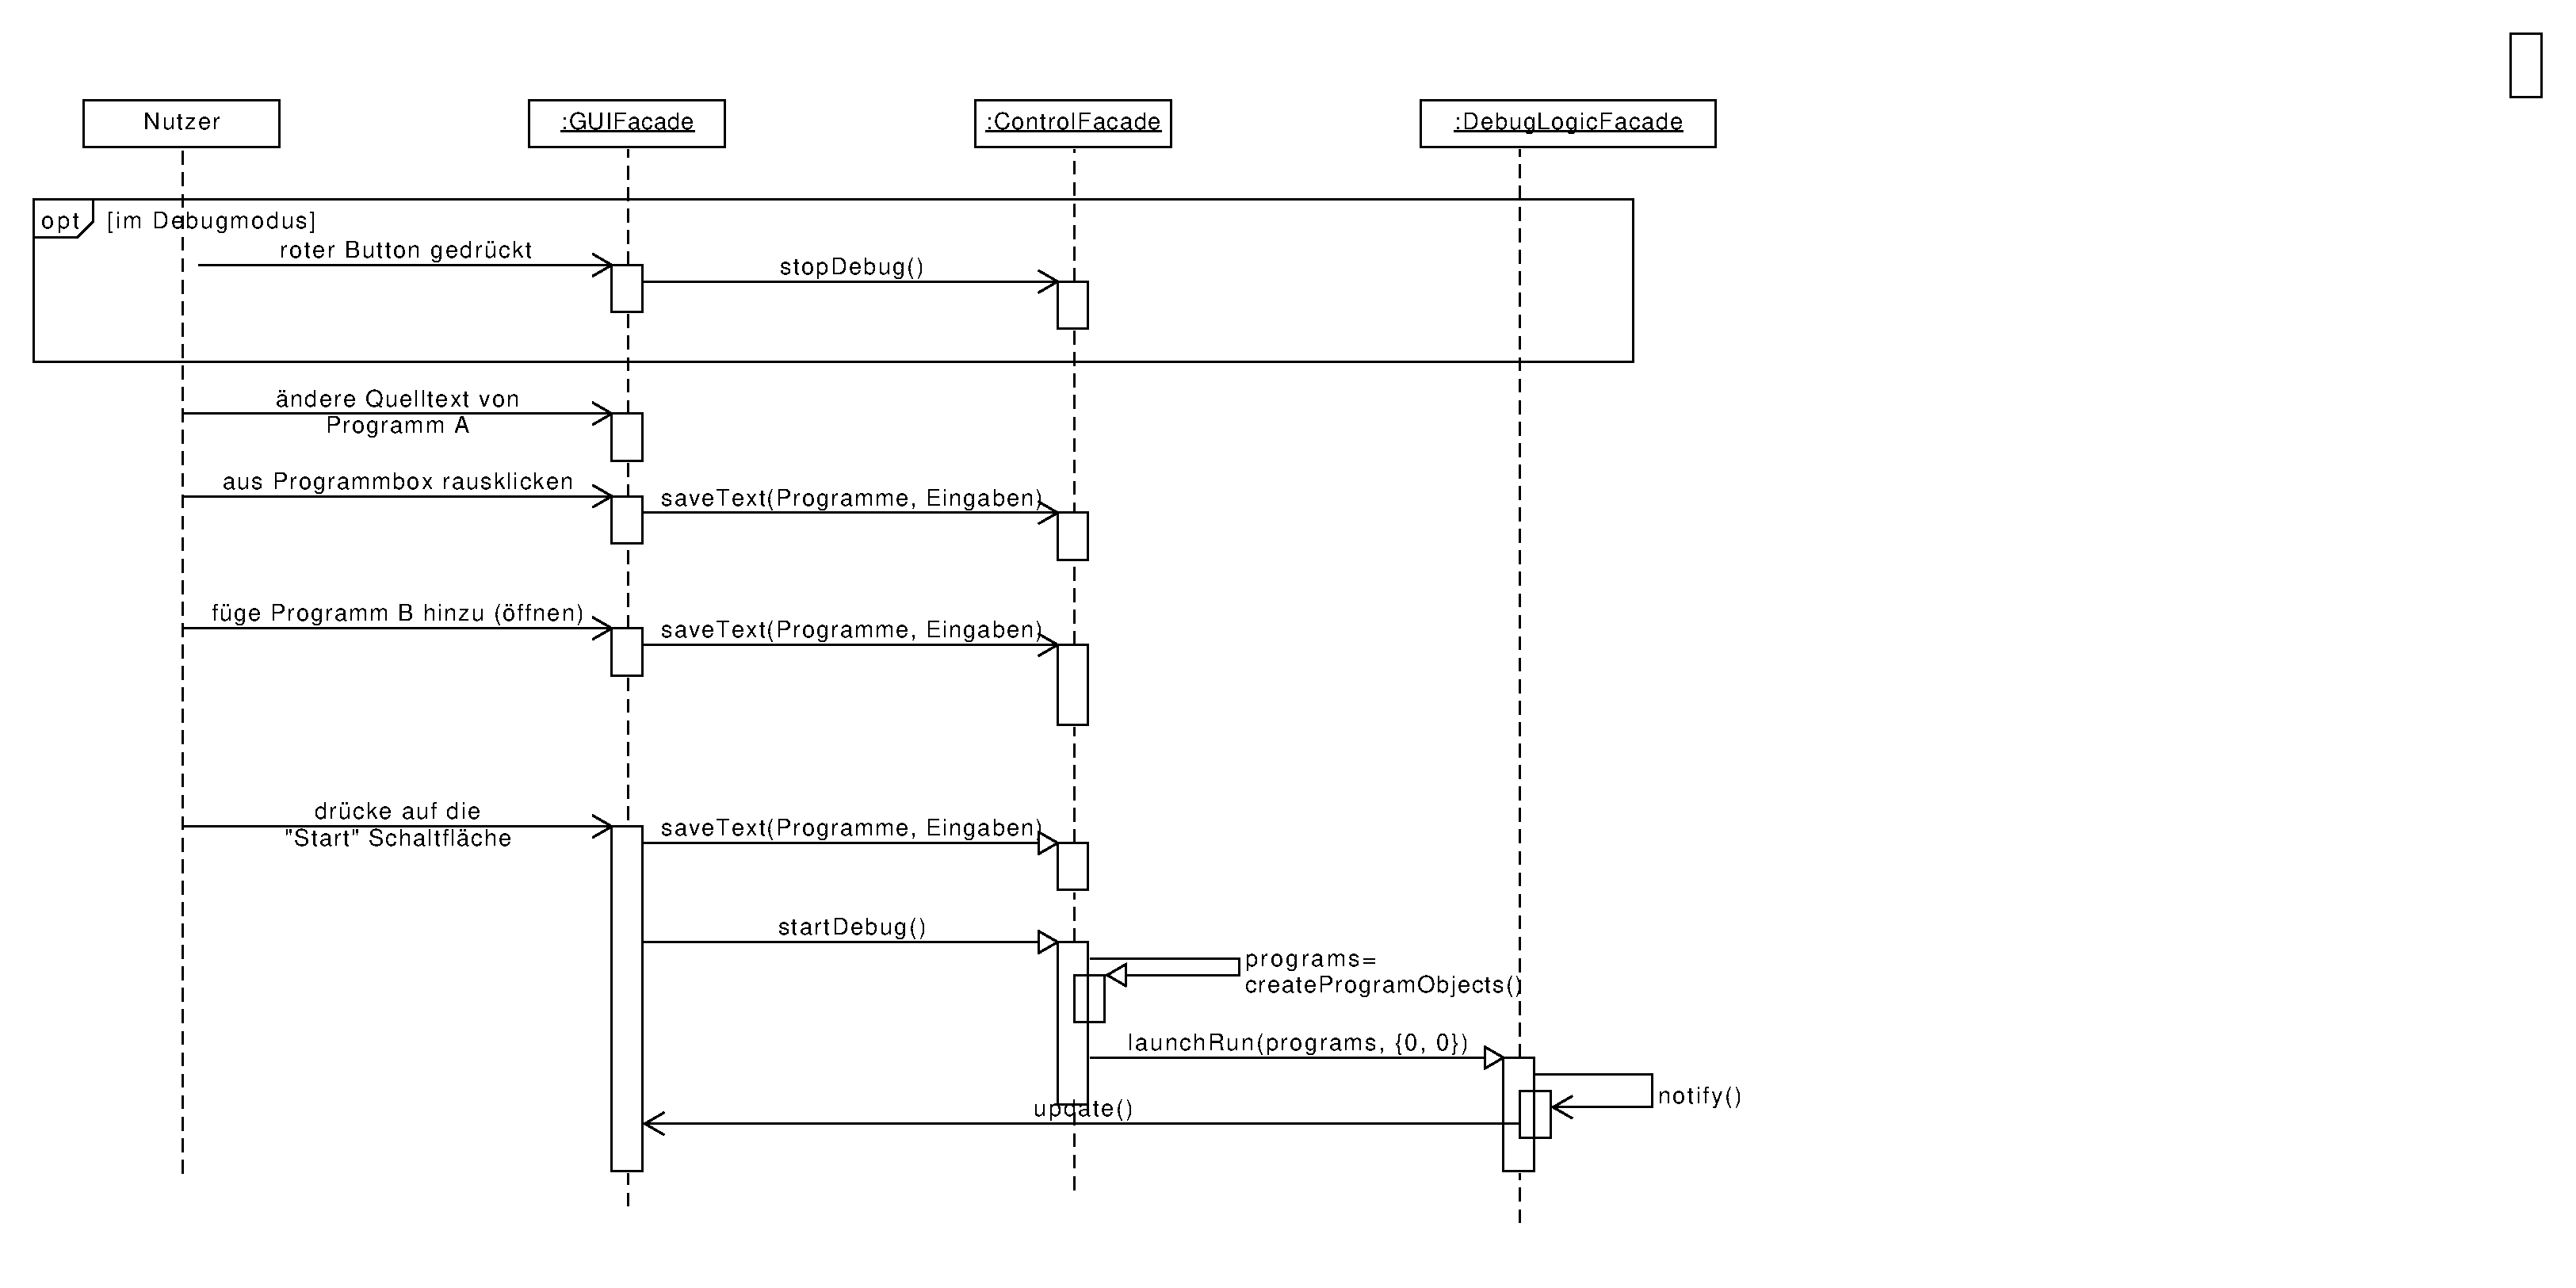
\includegraphics[width=0.8\textwidth]{diagrammIdeenUmlet/SequenceDiagrams/seq_AF20PDF.pdf}
\caption{Sequenzdiagramm: Ändern von Programmen}
\end{figure}
Möchte der Benutzer einen Programmtext editieren, muss er gegebenenfalls zunächst den Debugmodus beenden.
Anschließend lässt sich der Programmtext im Textfeld bearbeiten. Sobald der Benutzer außerhalb des
Textfelds klickt, gibt das MainInterface den neuen Programmtext und die Eingabeavariablen an die ControlFacade weiter. \\
Fügt der Benutzer einen neuen Programmtext durch Öffnen einer Datei hinzu, gibt das MainInterface diesen ebenfalls
mit den angegebenen Eingabevariablen an die ControlFacade weiter.\\
Sobald der Benutzer die Start-Schaltfläche auswählt um den Debugmodus zu starten, gibt das MainInterface erneut
alle eingegebenen Texte weiter und ruft schließlich startDebug() der ControlFacade auf. Diese erstellt aus den gespeicherten Informationen
Programm-Instanzen und gibt diese an die DebugLogicFacade weiter und startet damit den Debug-Lauf.

\newpage
\subsection{AF30: Setzen von Breakpoints}
\begin{figure}[!h]
\centering
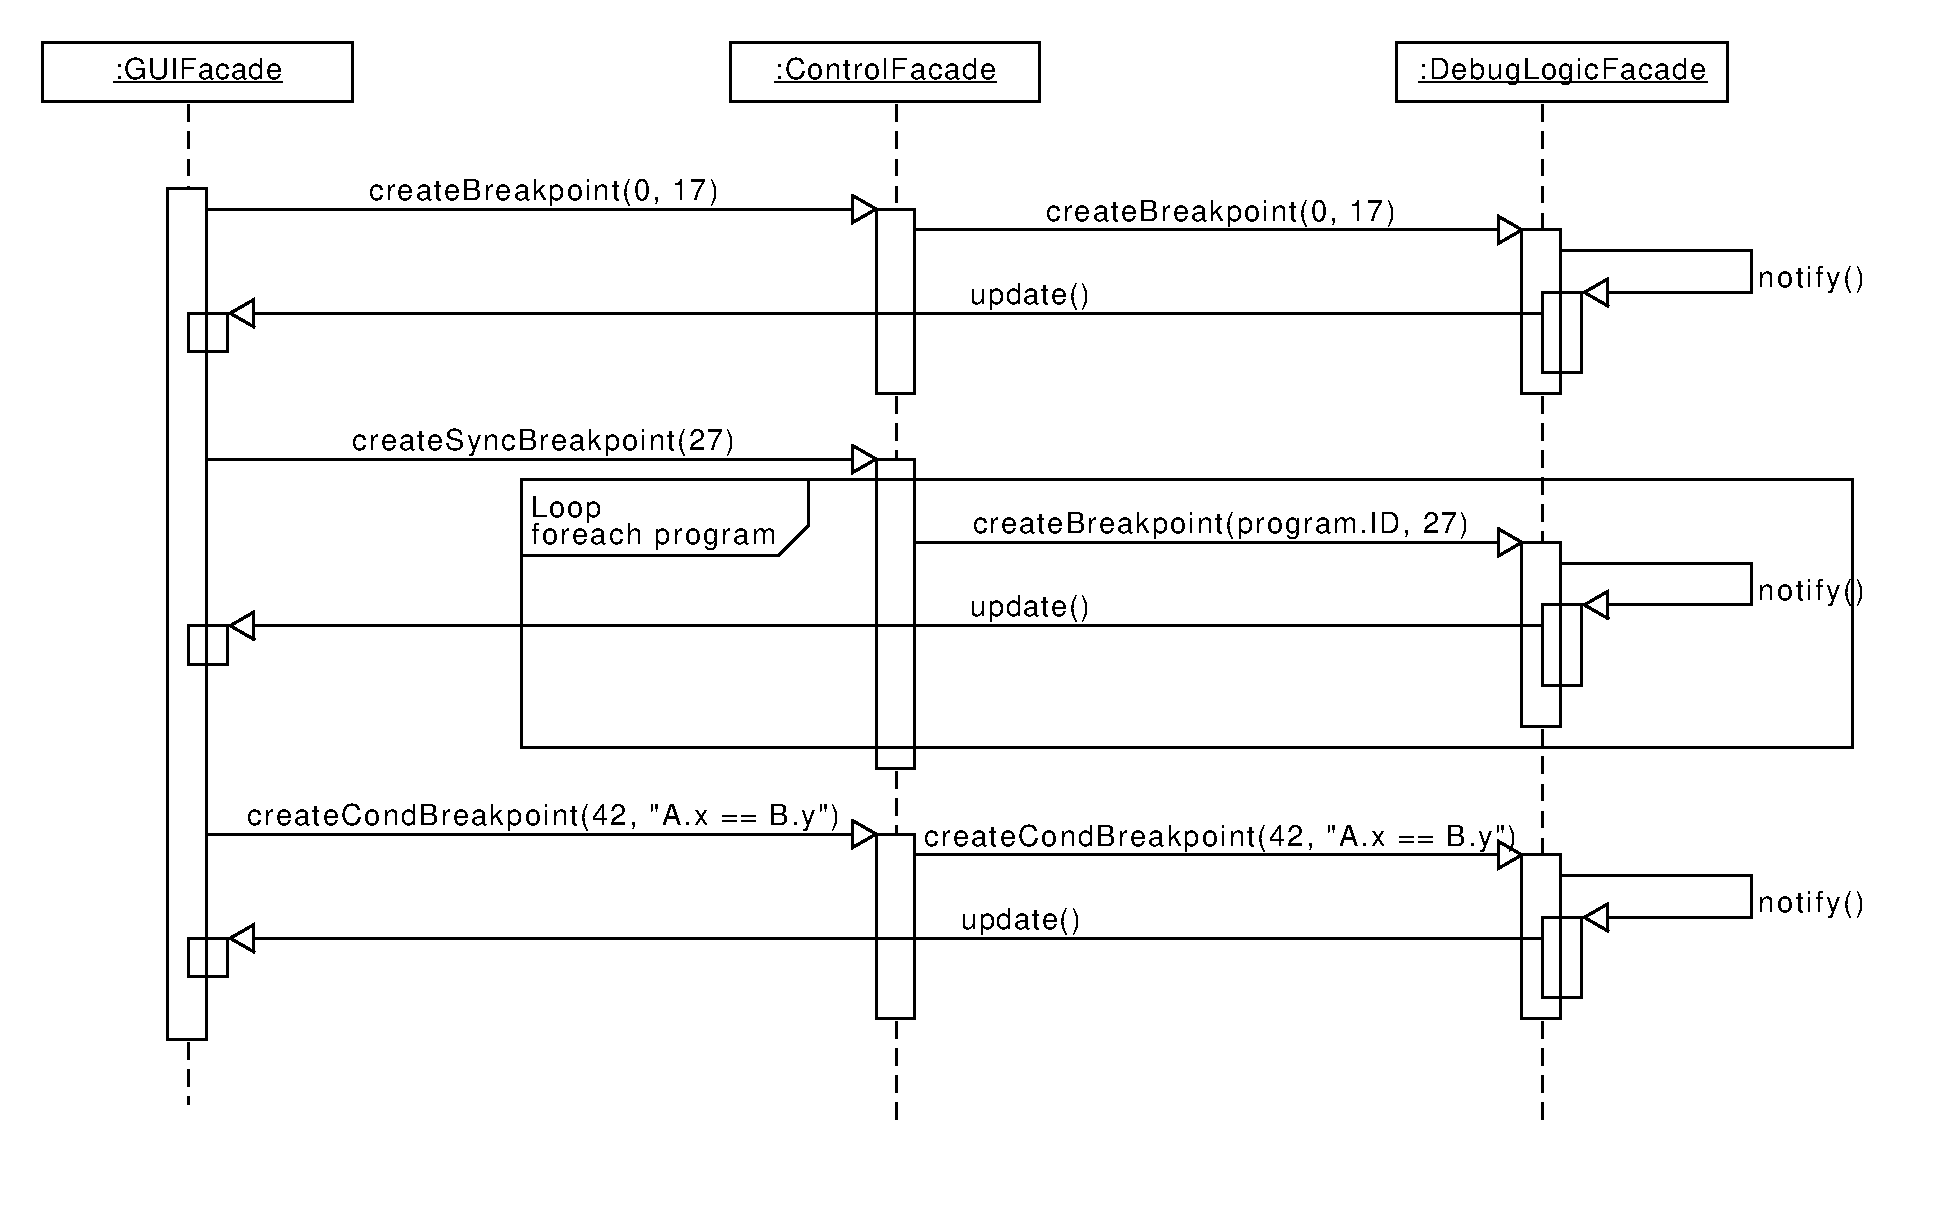
\includegraphics[width=0.8\textwidth]{diagrammIdeenUmlet/SequenceDiagrams/seq_breakpointsPDF.pdf}
\caption{Sequenzdiagramm: Setzen von Breakpoints}
\end{figure}
Setzt der Benutzer einen Breakpoint in eine Zeile in einem Programm, reicht das MainInterface
diese Information an die ControlFacade weiter, welche dann createBreakpoint mit der Programm-ID und der
Zeile an die DebugLogicFacade weitergibt.
Setzte der Benutzer jedoch einen Breakpoint in allen Programmen, teilt das
MainInterface dies der ControlFacade mit. Die ControlFacade ruft für jedes Programm
die Methode createBreakpoint der DebugLogicFacade auf.
Beim hinzufügen von bedingten Breakpoints gibt das MainInterface die ID des Breakpoints
und den vom Benutzer angegebenen Ausdruck an die ControlFacade weiter. Die Control reicht diese Informationen
ihrerseits an die DebugLogicFacade weiter, welche den Breakpoint ab diesem Zeitpunkt auswertet.

\newpage
\subsection{AF40: Hinzufügen von Watch-Expressions}
\begin{figure}[!h]
\centering
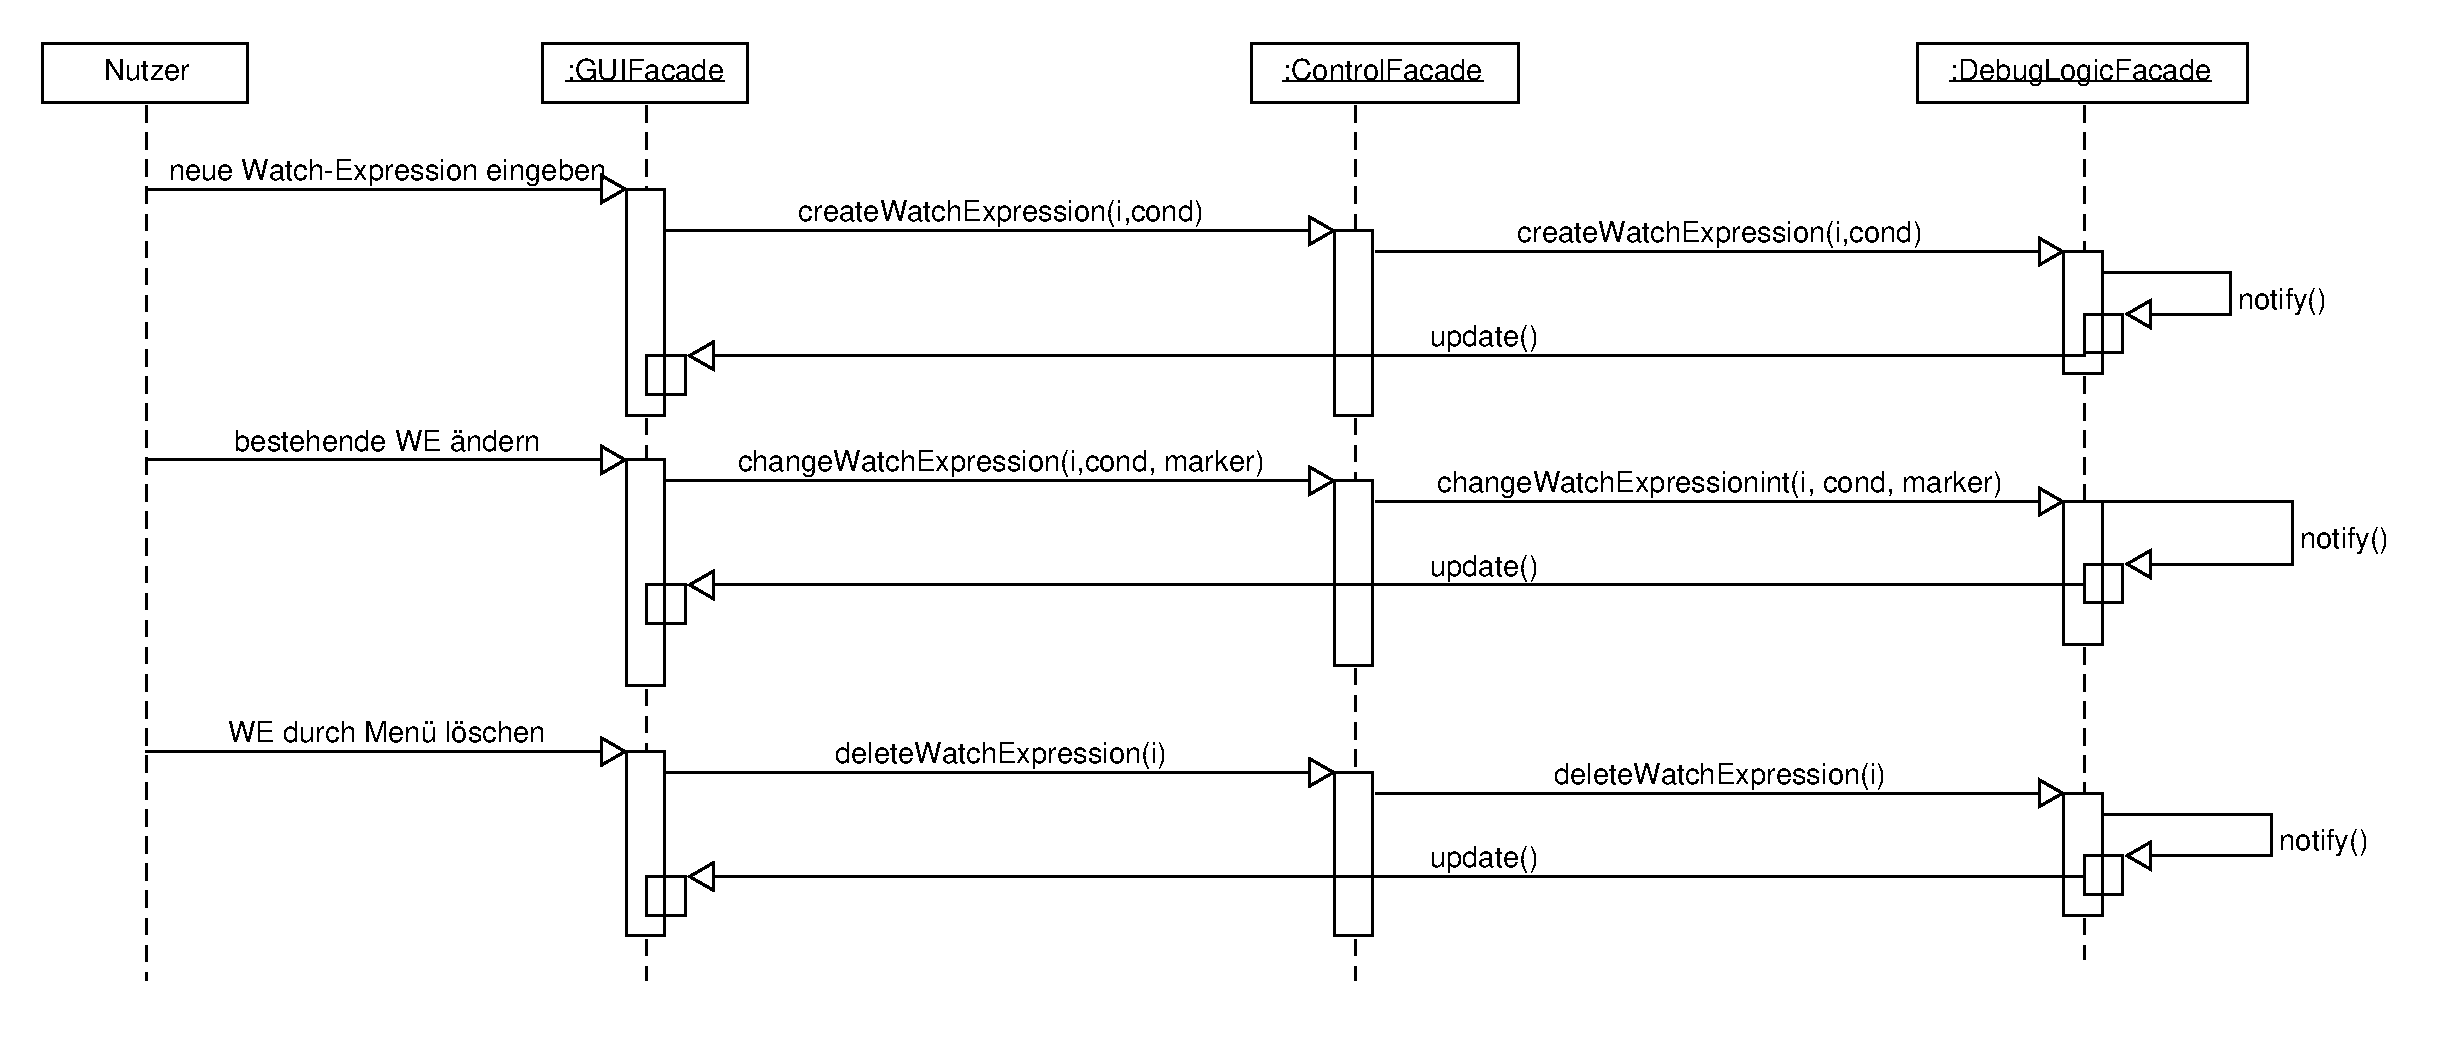
\includegraphics[width=0.8\textwidth]{diagrammIdeenUmlet/SequenceDiagrams/seq_WatchExpressionsPDF.pdf}
\caption{Sequenzdiagramm: Hinzufügen von Watch-Expressions}
\end{figure}
Diese Vorgänge sind für Watch-Expressions und bedingte Breakpoints identisch. \\
Gibt der Benutzer eine neue Watch-Expression an, wird die Bedingung und die ID vom MainInterface über 
die Control an die DebugLogicFacade weitergegeben. Ändert der Benutzer die Watch-Expression, zB indem 
er die Bereichsbindung angibt, wird dies ebenfalls über die Control an die DebugLogicFacade weitergegeben.
Auch beim Löschen einer Watch-Expression über das entsprechende Menü der Benutzeroberfläche, erhält die
DebugLogic diese Information über die Control und stoppt das Auswerten dieser Watch-Expression.

\newpage
\subsection{Generieren von Vorschlägen}%TODO
\begin{figure}[!h]
\centering
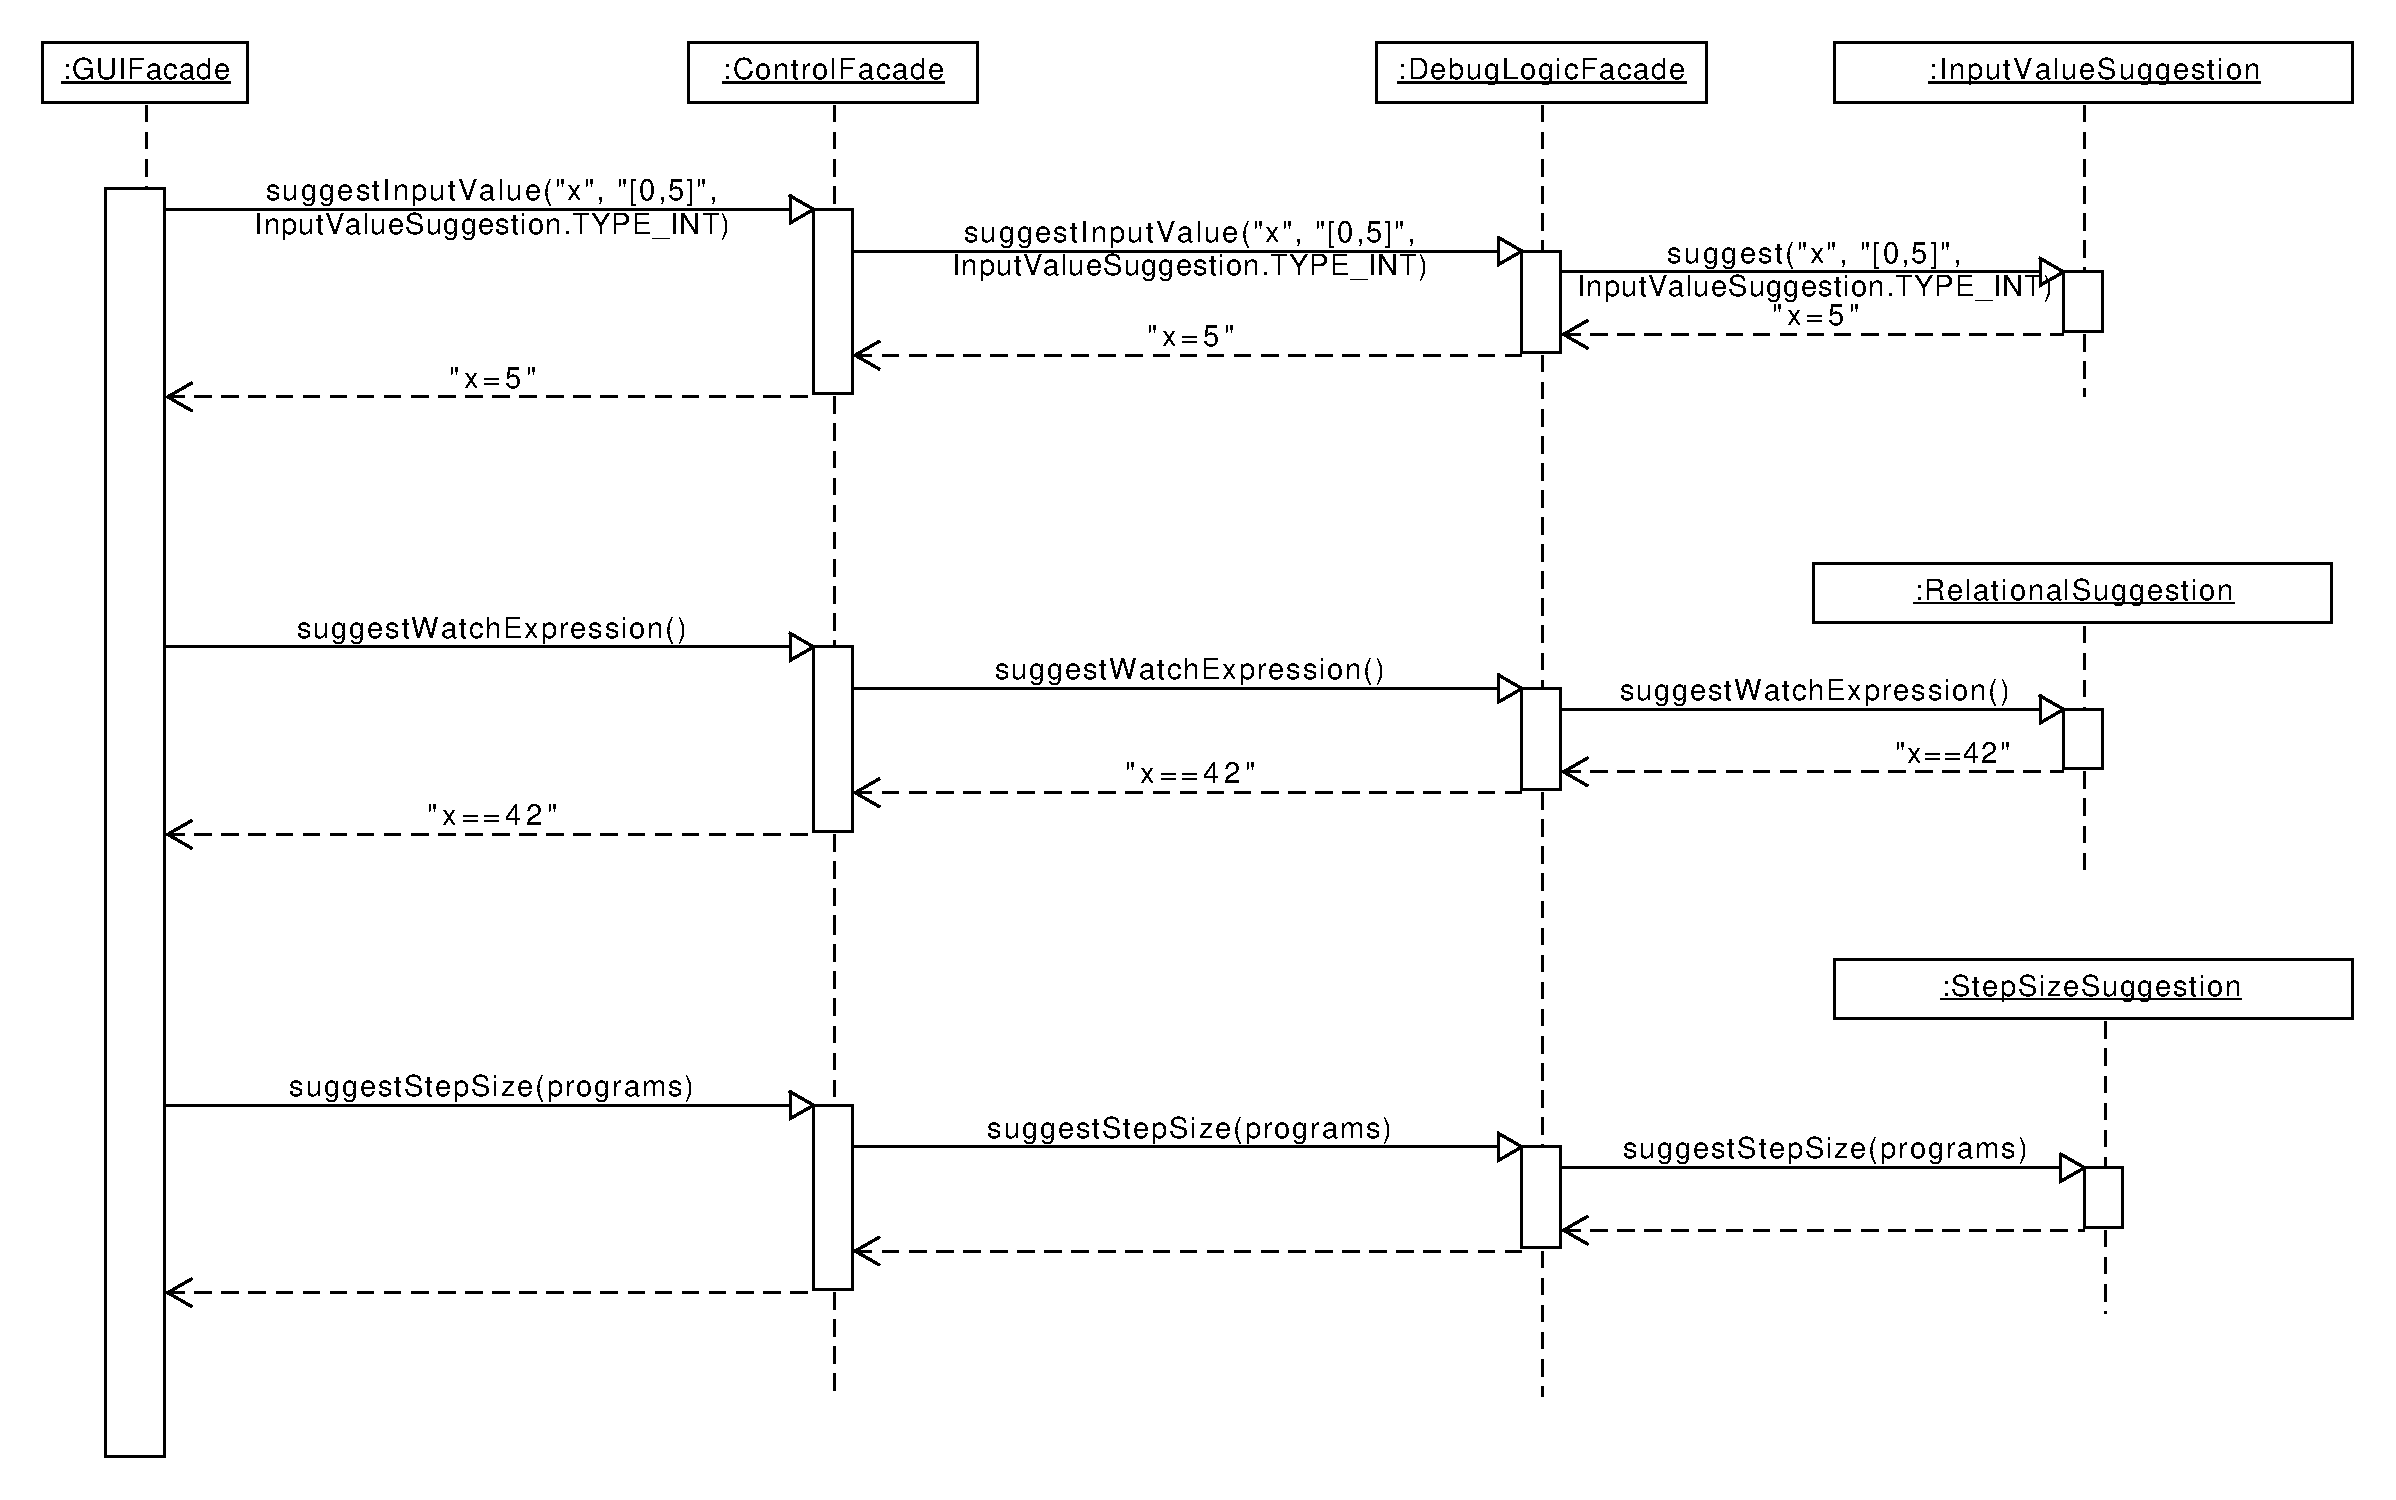
\includegraphics[width=0.95\textwidth]{diagrammIdeenUmlet/SequenceDiagrams/seq_suggestions.pdf}
\caption{Sequenzdiagramm: Generierung von Vorschlägen für Watch-Expressions}
\end{figure}
Möchte der Benutzer sich eine Watch-Expression vorschlagen lassen, so wird nach Anklicken des dazugehörigen Buttons der Befehl über die ControlFacade zur DebugLogicControl weitergeleiten. Dort wird dieser an eine Vorschlagsstrategie (z.B. EquivalenceSuggestionStrategy) gesendet und dort verarbeitet. Nachdem ein Vorschlag generiert wurde wird dieser als Zeichenkette, welche die finale Watch-Expression Bedingung repräsentiert, an die GUIFacade zurückgegeben. Danach fügt die GUI wie in AF40 eine Watch-Expression mit der erhaltenen Bedingung hinzu.

\newpage
\subsection{AF50: Programme debuggen}
\begin{figure}[!h]
\centering
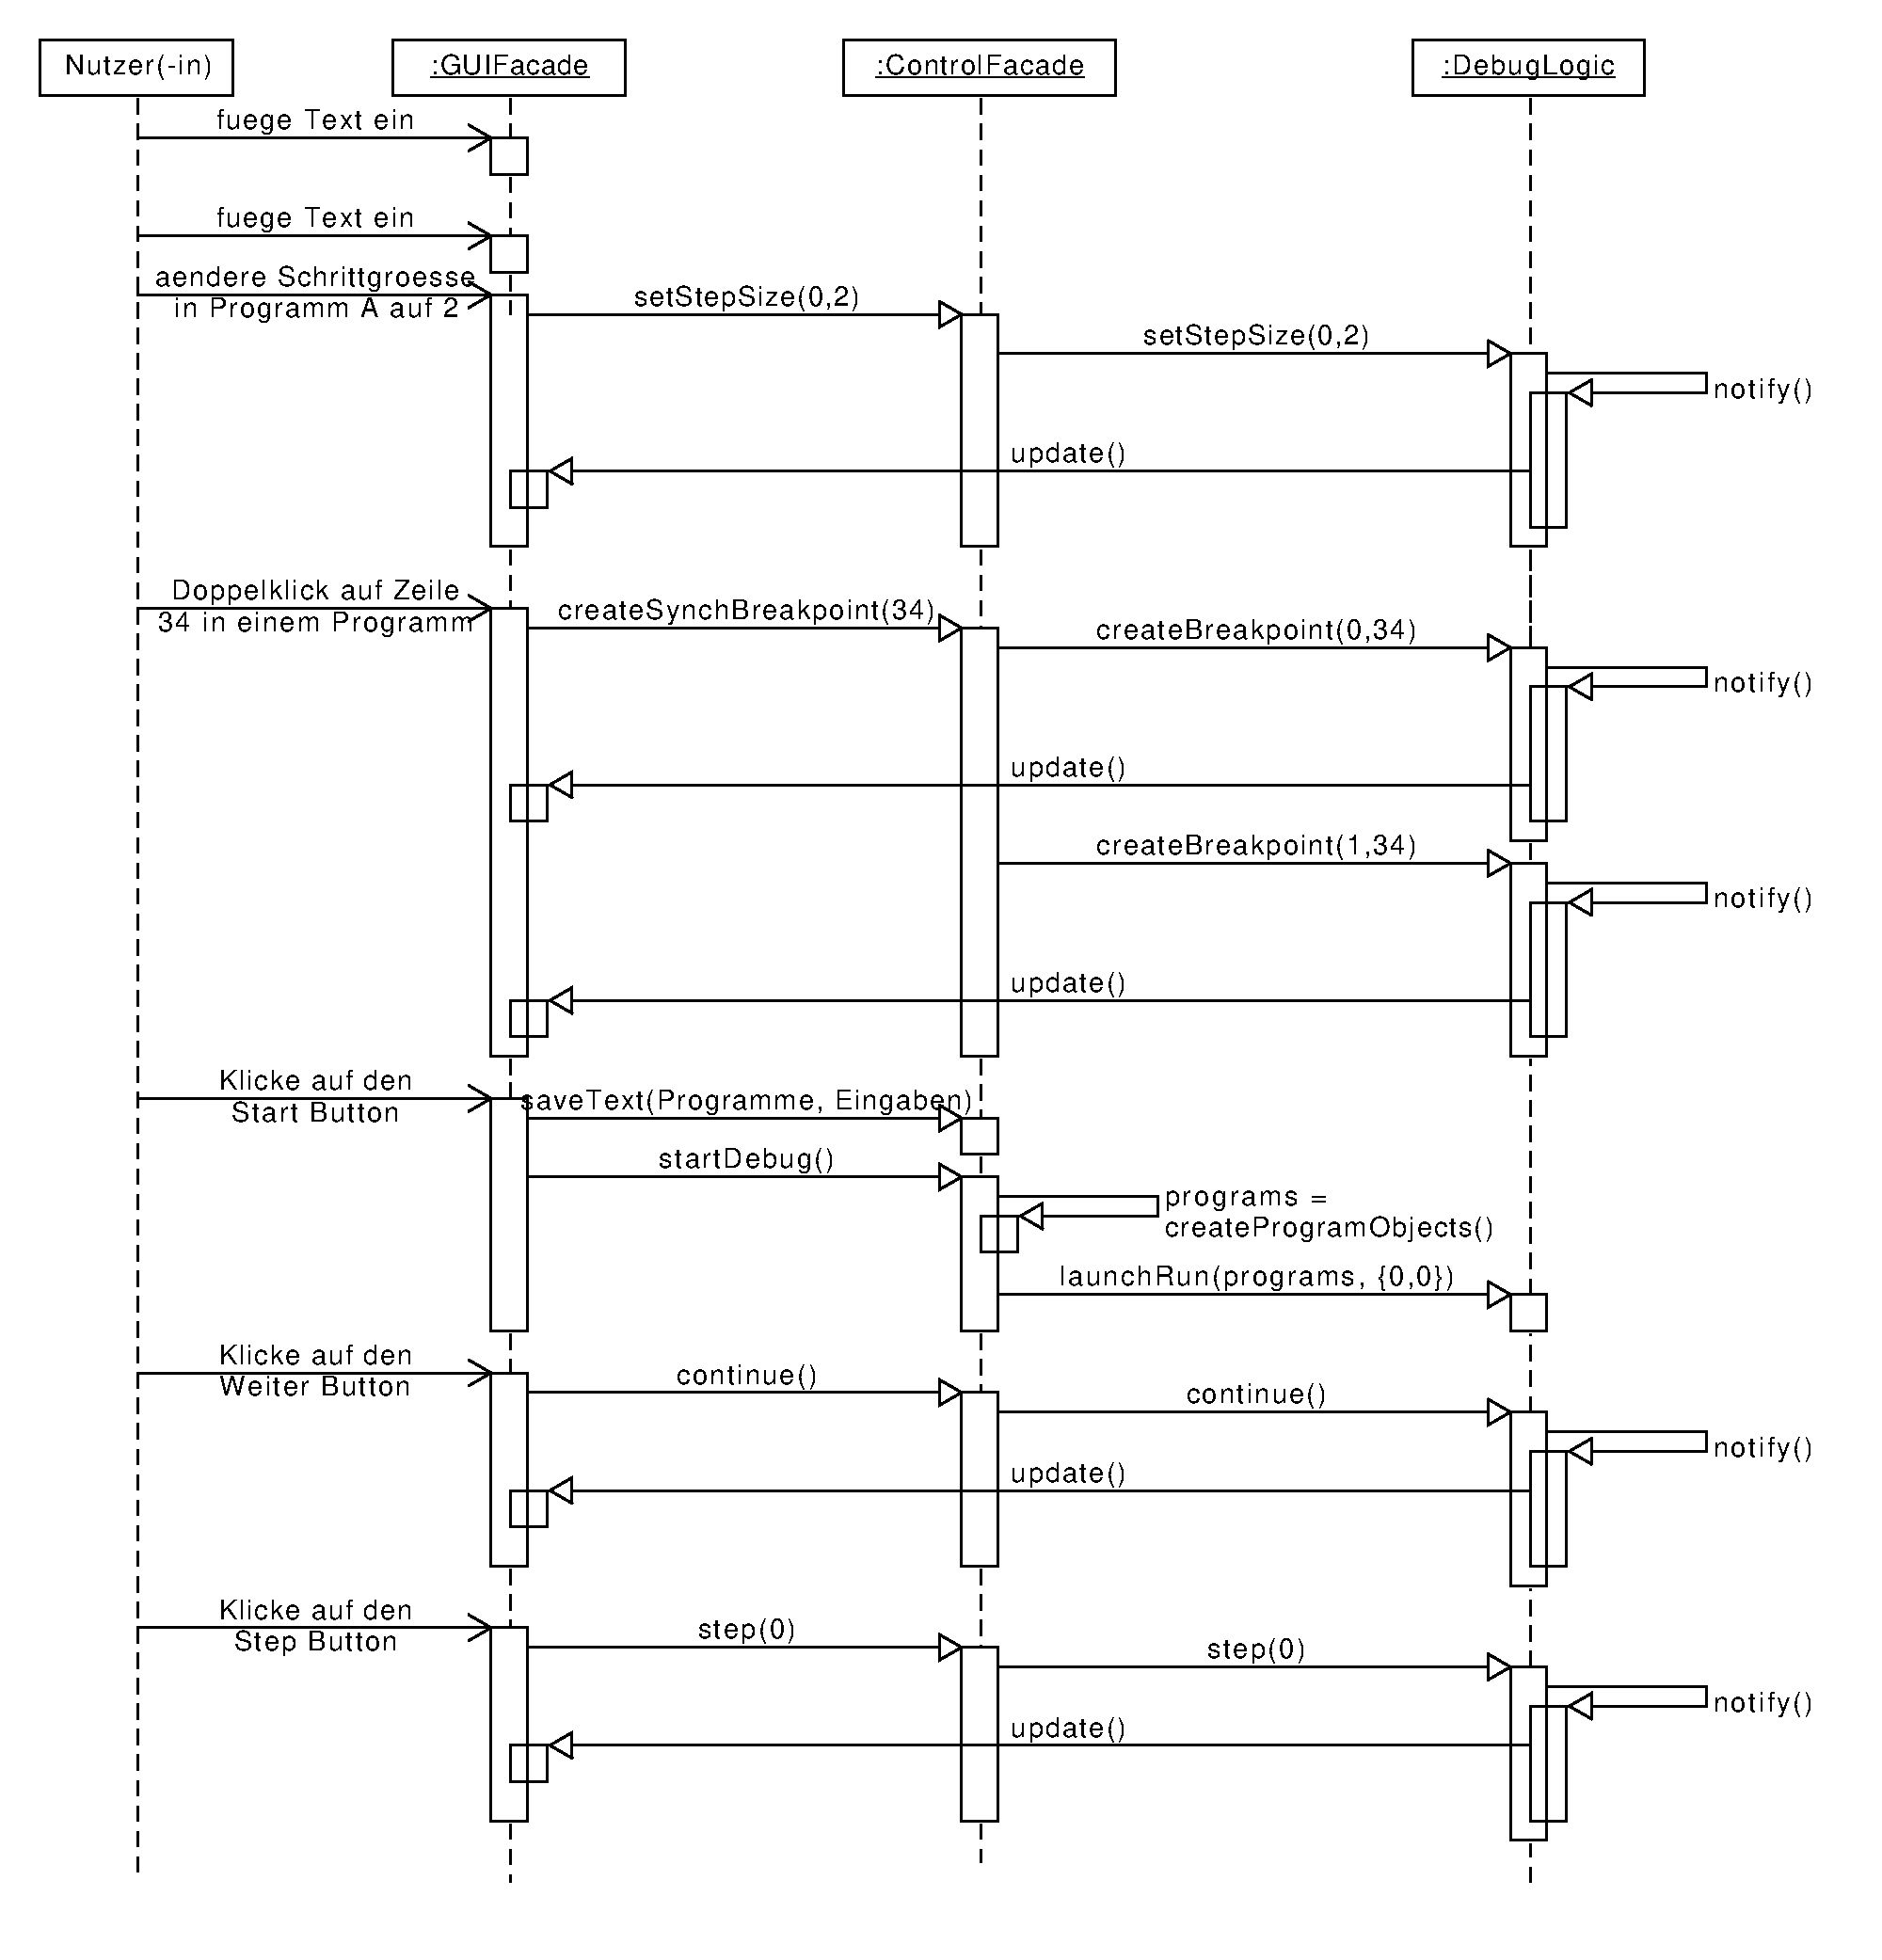
\includegraphics[width=0.8\textwidth]{diagrammIdeenUmlet/SequenceDiagrams/seq_AF50PDF.pdf}
\caption{Sequenzdiagramm: Debuggen von Programmen}
\end{figure}
Dieses Sequenzdiagramm fasst die Schritte des Nutzers bei einem Debug-Lauf zusammen.
Hierbei werden zuvor Programme hinzugefügt, die Schrittgröße geändert und Breakpoints hinzugefügt.
Sobald der Benutzer auf Start klickt, werden seine Eingaben final gespeichert und die Control startet 
den DebugLauf der DebugLogic.
Wenn der Benutzer durch Weiter oder Schritt durch den DebugLauf navigiert, werden diese Befehle über
die Control an die DebugLogic weitergegeben. Die Schritte werden von der DebugLogic ausgeführt, und anschließend
wird die GUIFacade als Beobachter dazu aufgefordert, die aktualisierten Werte anzuzeigen.
\subsection{Erzeugung abstrakter Strukturen im Subpaket Interpreter}
In diesem Abschnitt soll die Funktionalität des Subpaketes \textit{DebugLogic.Interpreter} beschrieben werden. Der Interpreter hat im Wesentlichen zwei Aufgaben: Einerseits muss er für WatchExpressions und bedingte Breakpoints eine abstrakte Struktur aufbauen, die sich einfach auswerten lässt. Andererseits hat er die Aufgabe, den kompletten Programmverlauf(im Folgenden \enquote{Trace})  eines Programmes zu berechnen und einen Iterator darüber bereitzustellen.
\subsubsection{Erzeugung einer abstrakten Repräsentation für Watch-Expressions und bedingte Breakpoints}
Watch-Expressions und bedingte Breakpoints bestehen immer aus einem vom Nutzer spezifizierten Ausdruck über den Variablen der vorkommenden Programme. Syntaktisch handelt es sich bei diesem Ausdruck einfach um einen Term. Semantisch muss aber bei bedingten Breakpoints sichergestellt sein, dass es sich um einen Term handelt, der sich zu einem Wahrheitswert auswertet. Wie Terme in der Klassenstruktur aufgebaut sind, ist im Kapitel \ref{Patterns} genauer beschrieben. Zusätzlich enthalten Watch-Expressions und bedingte Breakpoints einen Gültigkeitsbereich in Form von mehreren \textit{ScopeTuple}-Instanzen. 
\\
In den hier abgebildeten Diagrammen sind der Übersichtlichkeit halber nur die für die Erklärung wichtigsten Klassen meist ohne Methoden oder Attribute zu sehen.
Wir betrachten das Diagramm \ref{WEBBP}.  
\begin{figure}[!h]
\centering
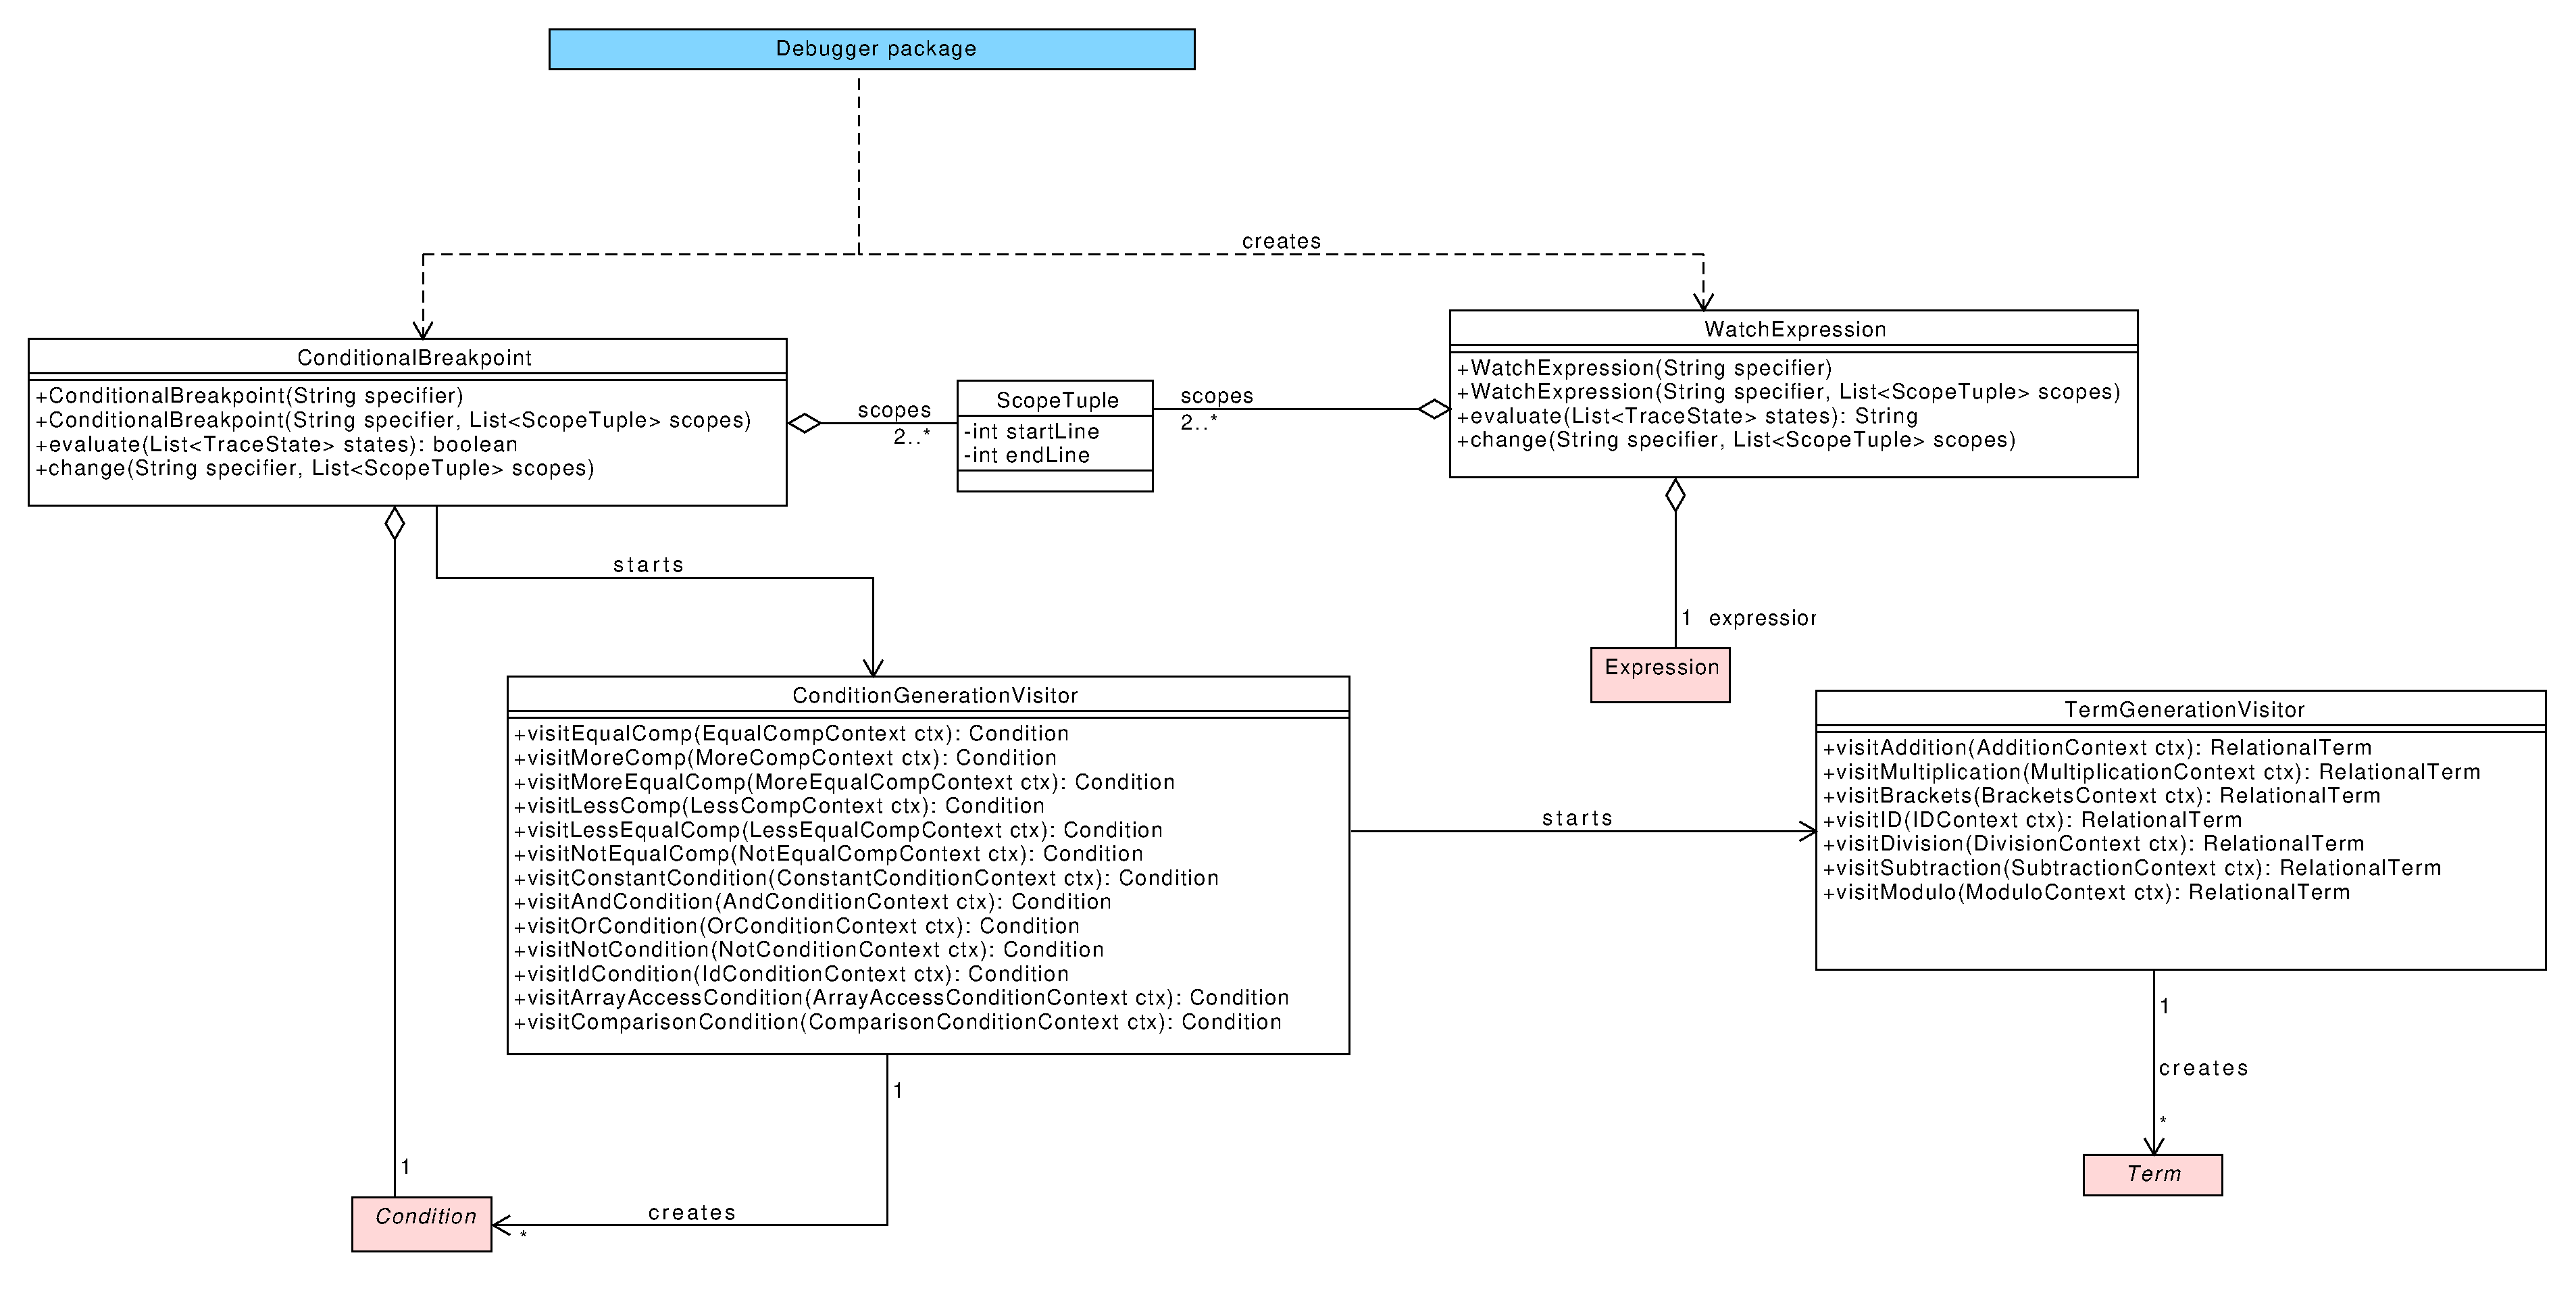
\includegraphics[width=1.2\textwidth]{diagrammIdeenUmlet/WatchExpressions.pdf}
\caption{Watch-Expressions und Bedingte Breakpoints}
\label{WEBBP}
\end{figure}
Das Debuggerpaket erzeugt einen neuen Bedingten Breakpoint und übergibt dazu eine Zeichenkette, die diesen spezifiziert. Der Bedingte Breakpoint nutzt das Paket \textit{AntlrParser}, um einen Syntaxbaum zu erzeugen. Dann wird ein \textit{TermGenerationVisitor} gestartet, der diesen Syntaxbaum abläuft und dabei eine \textit{Condition} erzeugt. Beim Erzeugen einer WatchExpression passiert das gleiche. Die Gültigkeitsbereiche können entweder bei Erzeugung direkt mitübergeben werden oder erst später durch Aufruf der \textit{change()}-Methode hinzugefügt werden. Standardmäßig ist der Gültigkeitsbereich maximal.
\newpage
\subsubsection{Erzeugung des Traces}
\begin{figure}[!h]
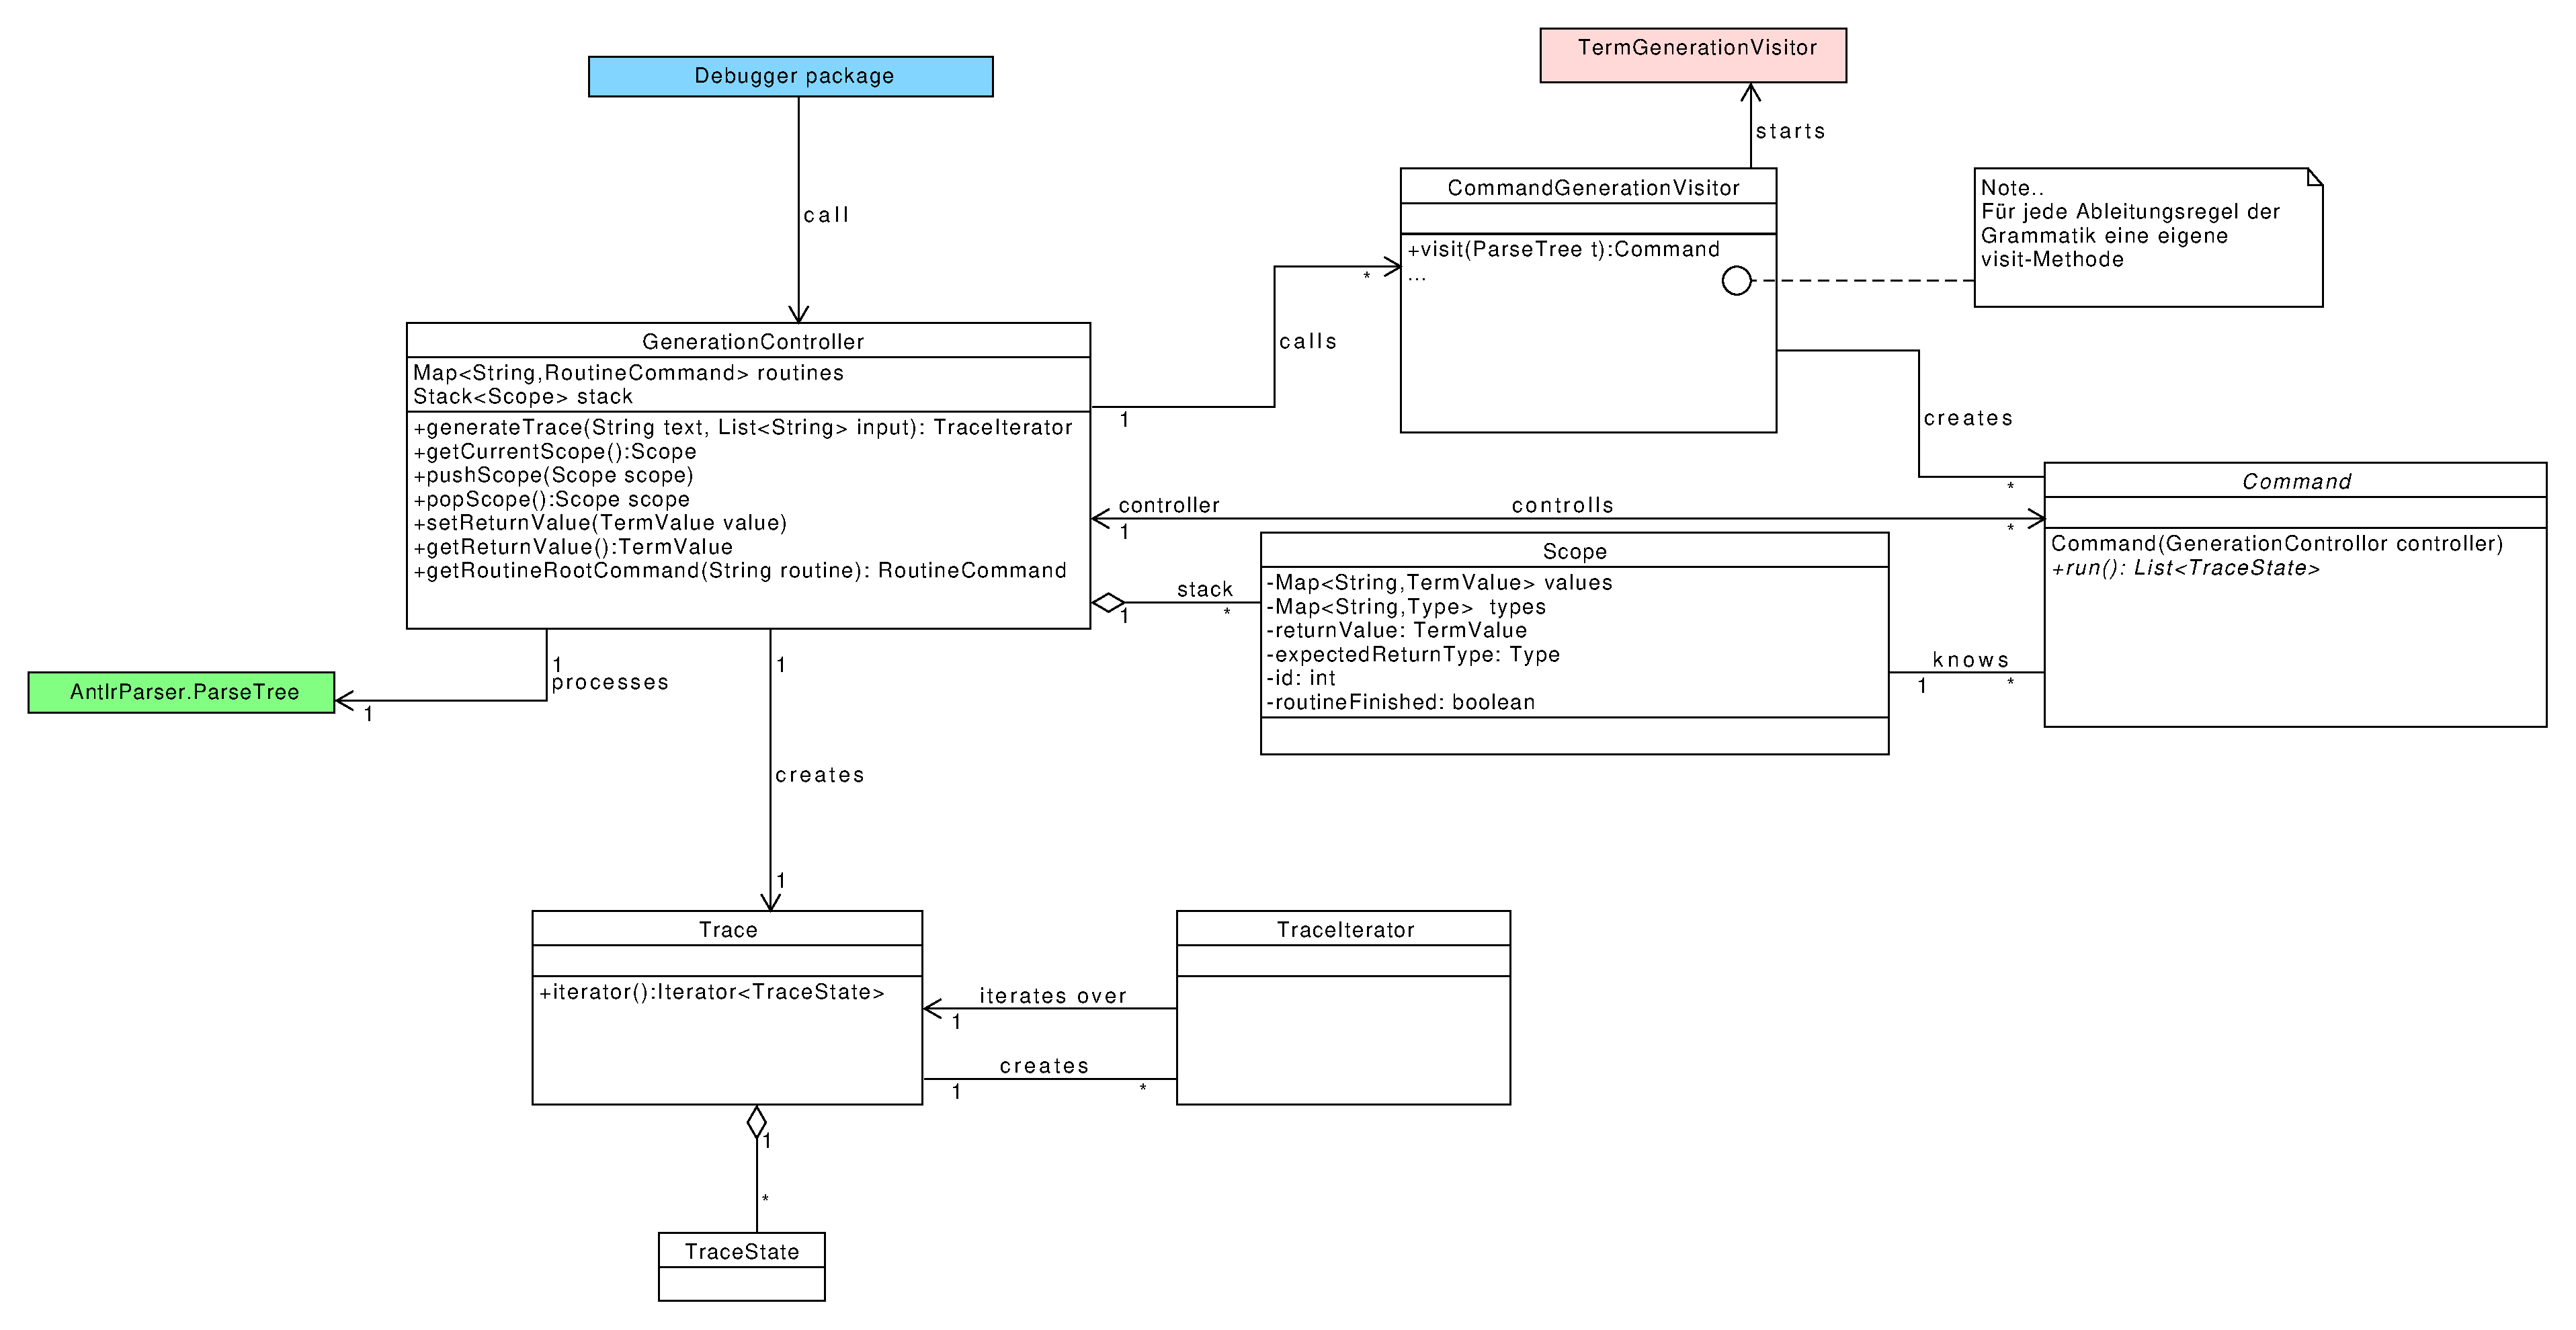
\includegraphics[width=1.2\textwidth]{diagrammIdeenUmlet/TraceGenerationClasses.pdf}
\caption{An der Tracegenerierung beteiligte Klassen}
\label{TraceGen}
\end{figure}
Gegeben sei das folgende (Wlang-)Programm:
\begin{verbatim}
int foo() {
    return 1+2+3;
}
int main(){
    int x;
    int y=3;
    while(x<(y+7)%4){
        x=x+1;
    }
    return c;
}
\end{verbatim}

Die Zusammenarbeit der in \ref{TraceGen} gegebenen Klassen soll nun an diesem Beispiel erklärt werden. 
Die Klasse \textit{GenerationController} steuert das Verfahren der Traceerzeugung. Sie bekommt in der Methode \textit{generateTrace()} den Quelltext und die Eingaben für diesen übergeben. Zunächst wird vom Subpaket \textit{DebugLogic.AntlrParser} ein \textit{ParseTree} erzeugt. Für obiges Beispielprogramm ist dieser in Abbildung \ref{ParseTreeExample} zu sehen.
\begin{figure}[!h]
\centering
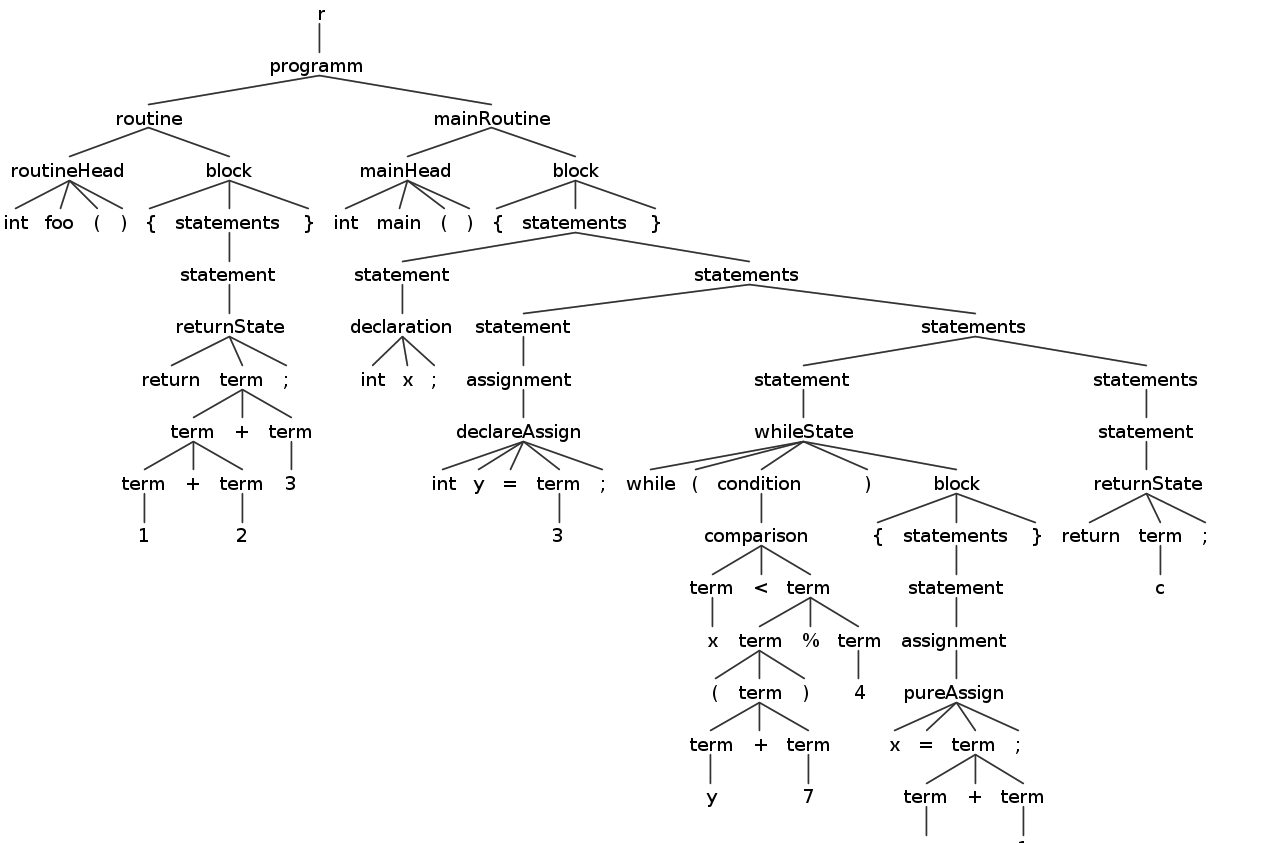
\includegraphics[width=0.95\textwidth]{diagrammIdeenUmlet/parseTreeExample.png}
\caption{Beispiel für einen Ableitungsbaum}
\label{ParseTreeExample}
\end{figure}
Über diesen Baum läuft der \textit{CommandGenerationVisitor} und erzeugt für jede Routine einen Baum aus Befehlen(\textit{Command}-Kompositum, siehe Kapitel \ref{Patterns}). Dabei verwendet er einen weiteren Visitor, die Terme in Form der in \ref{Terme} gegebenen Klassen erzeugen. 
Die Wurzeln dieser Bäume aus Befehlen werden im \textit{GenerationController} in der Map \textit{routines} gespeichert, sodass sie dann über ihren Routinennamen aufrufbar sind. Die Objektstruktur nach diesem Schritt sieht dann wie im Objektdiagramm \ref{CommandTreeExample} aus.
\begin{figure}[!h]
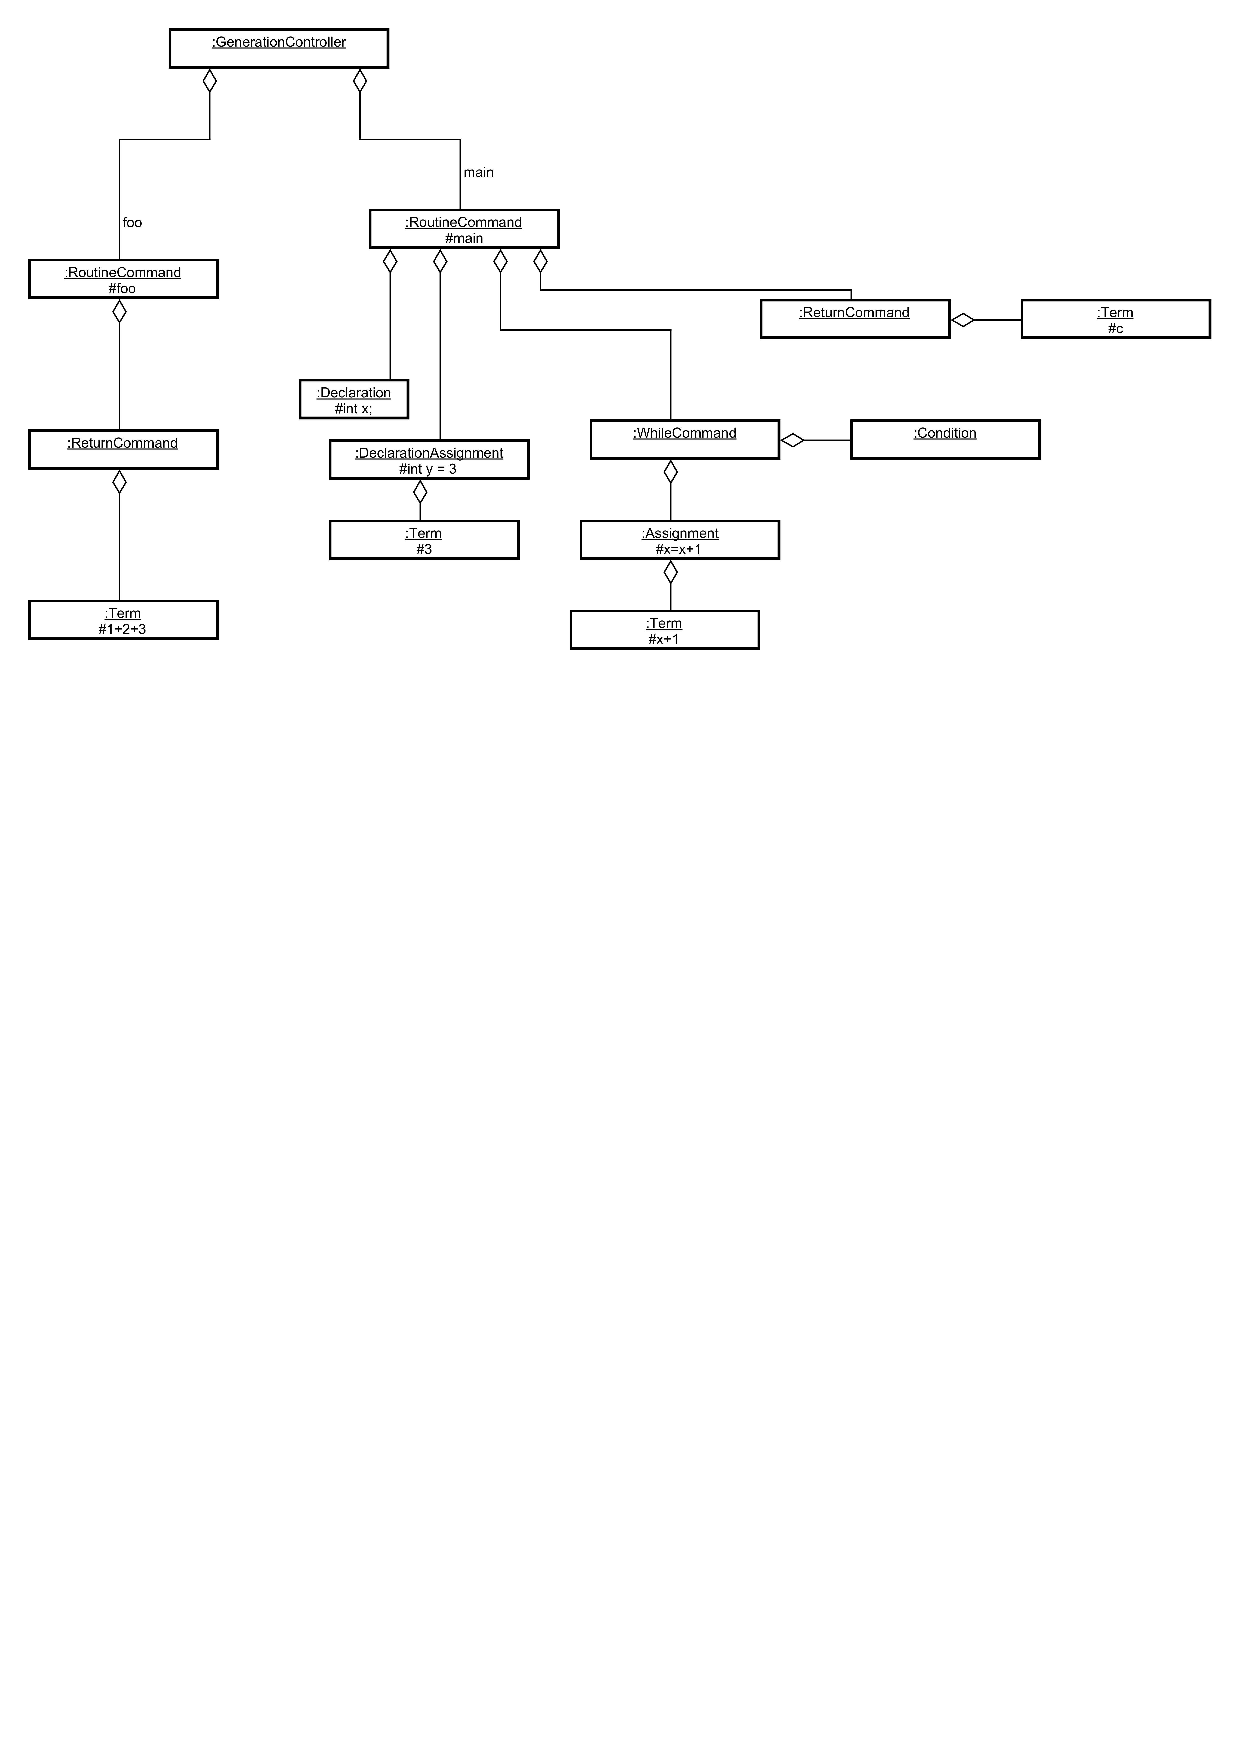
\includegraphics[width=1.2\textwidth]{diagrammIdeenUmlet/CommandTreeExample.pdf}
\caption{Objektstruktur nach der Commanderzeugung}
\label{CommandTreeExample}
\end{figure}
Die tatsächliche Ausführung der Commands folgt dann: Der \textit{GenerationController} enthält einen Stack aus \textit{Scope}-Objekten. In diesen Objekten ist alles über die zum aktuellen Ausführungszeitpunkt vorhandenen Daten gespeichert, etwa die Datentypen oder Werte der Variablen. Zu Beginn legt der \textit{GenerationController} einen \enquote{Urscope} auf seinen Stack. Dieser enthält lediglich die Eingabevariablen. Dann wird die \textit{run()}-Methode des Wurzelbefehls des Befehlsbaums der Mainroutine ausgeführt. Jeder Befehl ändert dann entprechend seiner Semantik die Werte im aktuell obersten Scope auf dem Stack. Dabei muss auch jeder Befehl eine entsprechende Typprüfung durchführen. Ein \textit{IfCommand} beispielsweise prüft seine Bedingung und führt seine Kinderbefehle im Baum aus, falls die Bedingung wahr ist. \\
Einen Spezialfall stellen die \textit{RoutineCall}-Commands dar. Ein solcher Befehl muss sich beim \textit{GenerationController} den Wurzelbefehl der passenden Routine holen, diesem die Argumente in Form einer Liste von \textit{Term}-Objekten übergeben, und diesen dann ausführen. Anschließend muss er sich vom \textit{GenerationController} den Rückgabewert holen. Dieser Wurzelknoten ist ein Objekt der \textit{Command}-Subklasse \textit{RoutineCommmand}. Solche Commands müssen bei Ausführung zunächst die Argumente holen, dann einen neues \textit{Scope}-Objekt auf den Stack legen, dann alle Kinder ausführen und danach den Scope wieder weglegen. Hierbei muss im Falle einer Funktion auch geprüft werden, ob ein Rückgabewert vorhanden ist.\\
Einen weiteren Spezialfall stellen \textit{ReturnCommand}-Objekte dar. Sie müssen im \textit{GenerationController} den Rückgabewert setzen und diesem mitteilen, dass die Routine beendet ist. Die darauffolgenden Befehle erkennen dies vor ihrerer Ausfühurung und führen sich nicht weiter aus. \\
Insgesamt gibt jeder Befehl nach der \textit{run()}-Methode eine Liste von  \textit{TraceState}-Objekten zurück. So gibt ein \textit{IfCommand}-Objekt also eine leere Liste zurück, falls die Bedingung nicht erfüllt ist, und die Konkatenation aller TraceStatelisten seiner Kinder sonst. Ein \textit{WhileCommand}-Objekt gibt dementsprechend die Listen seiner Kinder in wiederholter Form zurück. Die gesamte Liste verpackt der \textit{GenerationController} zu einem \textit{Trace}-Objekt und gibt einen \textit{TraceIterator} zurück.
\section{Abhängigkeitseinteilung mit Blick auf die Implementierung}
%Mit Blick auf den Implementierungsplan: Aufteilung in Klassen/Pakete, die unabhängig voneinander implementiert und getestet werden können.
\subsection{Abhängigkeiten}
Das Paketdiagramm besagt, dass FileHandler und DebugLogic nicht voneinader abhängen.
Beide werden von der Control benutzt und müssen somit korrekt implementiert sein, bevor die Control richtig funktionieren kann. Weiter führt die Control Methoden der GUIFacade aus, ist aber nicht von derer Abhängig, da diese nicht relevant ist für eine funktionierende Control.
Die GUI hingegen ist stark von der Control abhängig und kann ohne diese nicht korrekte Daten anzeigen.

%TODO Pakete der Debuglogic aktualisieren, da noch nicht fertig
\subsection{Implementierung}
Die Implementierung der Hauptpakete kann durch den von Fassaden geprägten Entwurf und dem MVC-Konzept gleichzeitig geschehen. Es ist jedoch sinnvoll das Exception Paket als erstes zu implementieren, um später keine Stellen im Quelltext suchen zu müssen, an denen Fehler auftreten können.
Weiter sollten die Unterpakete der DebugLogic entsprechend der Benutztrelation implementiert werden, also zuerst AntlrParser, Interpreter und zum Schluss der Debugger.
Dieses Problem besteht bei den Hauptpaketen nicht, da für die Kommunikation ausschließlich Fassaden benutzt werden. Diese können zur gleichzeitigen Implementierung der Pakete als Stummel pseudoerstellt werden, d.h. die Methoden sind leer und enthalten keine bzw. nur sehr wenig Funktionalität.\\
Der FileHandler stellt wiederum eine Ausnahme dar, da er mehrere Klassen zur Repräsentation und Interaktion zum Dateisystem bereitstellt.
Hierbei müssen die Klassen ConfigurationFile, PropertiesFile und LanguageFile gleichzeitig mit der FileHandlerFacade Klasse einsatzbereit sein.

\begin{figure}[!h]
\centering
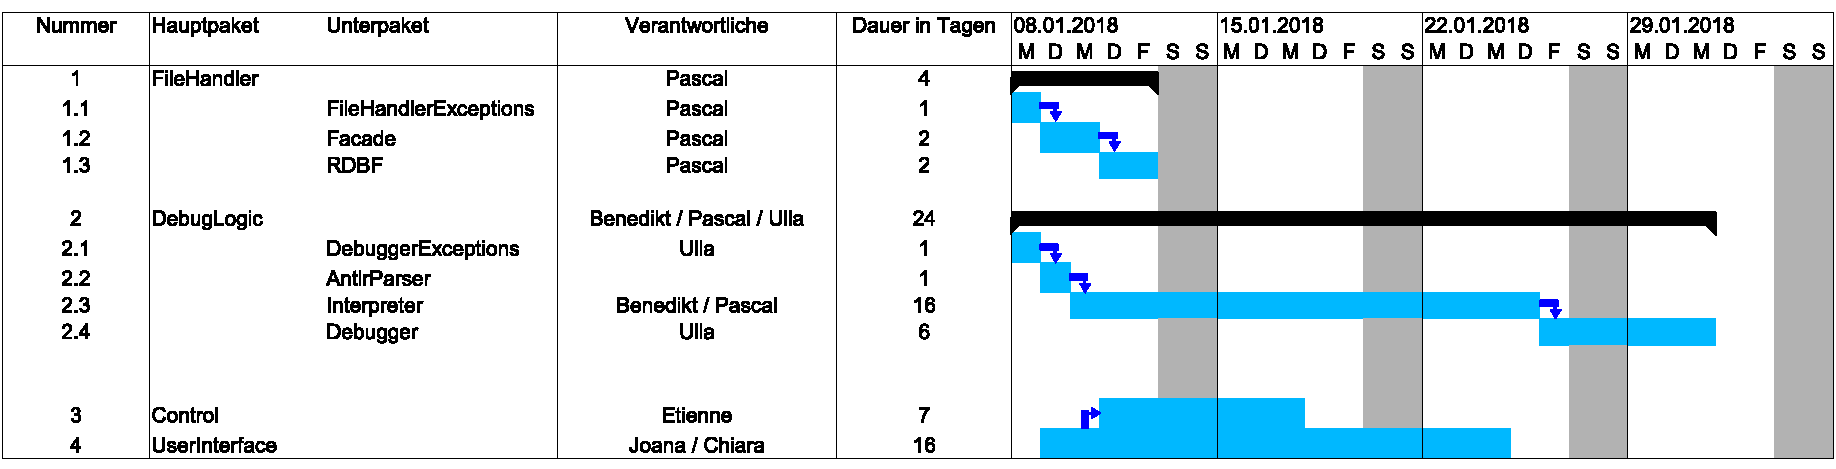
\includegraphics[width=1.0\textwidth]{GanttDiagramm_withArrows.pdf}
\caption{Gantt Diagramm: Zeitplanung der Implementierung}
\end{figure}


\section{Programmsprache, Antlr und Speicherformat}\label{FormSpez}

\subsection{Wlang}

Wlang ist eine prozeduale, imperative Sprache, welche weder objektorientiert, noch einrückungsbasiert ist. \\
Sie unterstützt die primitiven Datentypen int, long, float, double, char und boolean mit den selben Genauigkeiten wie Java.
Außerdem sind  bis zu dreidimensionale Arrays dieser Datentypen möglich. \\
Desweiteren unterstützt Wlang Kontrollstrukturen wie Funktionen und Prozeduren, die bedingten Ausführungen if, else if und else und while-Schleifen. \\
Es muss in jedem Programm eine main-Routine vorhanden sein, von der die Ausführung ausgeht. Routinen, die aufgerufen werden, müssen darüber stehen. Kommentare können
sowohl zeilenweise (//) als auch zeilenübergreifend (/*Kommentar*/) benutzt werden.
Sämtliche Variablen müssen innerhalb einer Routine stehen. Auch Rekursion ist möglich. \\
Für die Definition der Kontextfreien Antlr-Grammatik siehe Anhang.


\subsection{Verwendung von Antlr}

Wie bereits im zweiten und dritten Kapitel beschrieben, benutzt der DIbugger im Paket \textit{DebugLogic.AntlrParser} extern erzeugte Java-Klassen, um die textuelle Nutzer-Eingabe zu einem ablaufbaren \textit{Parse Tree} umzuwandeln. Diese Klassen werden von dem frei verfügbaren Programm Antlr\textsuperscript{\textcopyright} (Version 4) erzeugt.
Ein \textit{Parse Tree} (manchmal auch \textit{Syntax Tree} genannt) ist dabei ein Baum mit einer eindeutigen Wurzel, der die syntaktische Struktur eines Textes – in diesem Fall der Nutzereingabe – mit Hilfe einer kontextfreien Grammatik darstellt. Die Spezifikation der Grammatik findet sich im Anhang.

Auf Basis der Grammatik generiert Antlr mehrere Java-Klassen, wie einen Lexer, einen Parser, sowie einen Visitor und ein Visitor-Interface. Die Funktionalität dieser Klassen wird im Unterpaket \textit{DebugLogic.Interpreter} genutzt und erweitert.

%TODO wie und wo werden diese weiter modifiziert?

\subsubsection{Vorteile der Verwendung eines Parser-Generators}
Die Verwendung eines Parser-Generators wie Antlr im Allgemeinen hat mehrere Vorteile gegenüber einem “von Hand” geschriebenen Parser: Offensichtlich spart es Zeit und Ressourcen, die in die Entwicklung des eigentlichen Produktes gesteckt werden können. Nicht zu vernachlässigen ist auch, dass Änderungen an der Grammatik zunächst nur in der Grammatik selbst gemacht werden müssen und nicht sofort Änderungen in mehreren, möglicherweise sehr großen Klassen nach sich zieht. Zuletzt ermöglichen Parser-Generators wie Antlr, dass man ein Projekt auf einem Parser aufsetzt, der bereits von einer großen Gruppe an Nutzern getestet wurde, und so die Fehleranfälligkeit reduziert.


\subsubsection{Anforderungen an den verwendeten Parser-Generator}

Mindestanforderungen an einen Parser-Generator für dieses Projekt waren Java-Kompatibilität, Kostenfreiheit und eine offene Lizenz, die mit der vom DIbugger verwendeten Lizenz kompatibel ist.

Antlr kann Java-Code produzieren, ist kostenlos und unter BSD-Lizenz veröffentlicht.
Obwohl es auch andere Parser-Generator gibt, die diese Anforderungen erfüllen, spricht für Antlr, dass es auf allen Betriebssystemen läuft, in eine Entwicklungsumgebung eingebunden werden kann, eine aktuelle Version mit gutem Support bereitstellt und viele Online-Ressourcen dazu verfügbar sind.
Diese Faktoren erleichtern dabei nicht nur die gegenwärtige Entwicklung des Produkts sondern auch zukünftige Erweiterungen.

\subsection{RDBF Speicherformat}
RDBF ist ein nicht einrückungsbasiertes, imperatives Speicherformat, welches das Speichern von komplexen Blockstrukturen erlaubt.
Eine Blockstruktur besteht aus einem Blocknamen und Rumpf, welcher in sich wieder mehrere Blöcke und Daten haben.
Daten bestehen aus einem Namen, Wert und Typ, welcher aber erst von einem Parser herausgefunden werden muss.
Es werden die Datentypen String, int, long, float, double und boolean unterstützt.
Weiter gibt es einen spezialisierten TextBlock, der nur einen Fließtext zum Speichern enthält.
Kommentare können durch das Kennzeichnen am Anfang einer Zeile mit \enquote{//} erzeugt werden.
Das Speicherformat ist durch eine Kontextfreie Grammatik definiert. Diese kann in Kapitel 9.4 eingesehen werden. 

\section{Änderung zum Pflichtenheft}
\paragraph{Erweiterte Syntax für Watch-Expressions und bedinge Breakpoints}
In Kapitel 12.8 des Pflichtenheftes wurde die Syntax der Watch-Expressions und bedingter Breakpoints durch eine kontextfreie Grammatik definiert. 
In dieser Grammatik war kein bedingter Breakpoint der Form $A\&\&B$ bzw. $A||B$ oder $!A$ ableitbar. Diese Einschränkung ergab sich als während des Entwurfs als nicht notwendig und wird demnach aufgehoben. Eine genaue Definition der Watch-Expressions und bedingten Breakpoints in Form einer Antlr-Grammatik ist im Anhang zu finden. Insgesamt können diese auf syntaktischer Ebene aus beliebigen Termen bestehen. 




\section{Anhang}
%TODO UML-Klassendiagramm 

Startnichtterminal in den Grammatiken ist immer die Variable \textit{r}.
\subsection{Kontextfreie Antlr-Grammatik für WLang-Syntax}
\begin{verbatim}

grammar Wlang;
r: programm;


programm: routine* mainRoutine;
routineHead: returntype = TYPE id = ID '(' args=arglist? ')' #FunctionHead
			| 'void' id =ID '('args=arglist?')' #ProcedureHead
			;

mainHead: returntype = TYPE 'main' '(' args=arglist? ')' #MainFunctionHead
			| 'void' 'main' '('args=arglist?')' #MainProcedureHead
			;

arglist: argument ',' arglist | argument;
argument: type=TYPE id=ID;
filledArglist: filledArgument ',' filledArglist | filledArgument;
filledArgument: term;
routine: routineHead block;
mainRoutine: mainHead block;

//Statements

statements : statement statements #CompStatement 
			| statement #SingleStatement
			;
statement:  ifState 
		| ifelseState 
		| whileState 
		| assignment
		| arrayDeclaration
		| arrayDeclareAssign
		| arrayElementAssign
		| declaration 
		| funcCall ';'	
		| returnState;
		

funcCall: functionname = ID '(' args=filledArglist? ')' 
	  |functionname = 'main' '(' args=filledArglist? ')'
	;

	
block: '{'statements'}';
assignment: declareAssign
			| pureAssign
			;

arrayDeclaration: type = TYPE dims id = ID ';';
arrayDeclareAssign: type = TYPE dims id = ID ASSIGN '{'filledArglist'};';
arrayElementAssign: arrayAccess ASSIGN value = term';';
dims: '['term']' #oneDims
	| '['term']''['term']' #twoDims
	| '['term']''['term']''['term']' #threeDims
	;


pureAssign: id = ID ASSIGN value = term ';';
declareAssign: type = TYPE id = ID ASSIGN value = term ';';
declaration: type = TYPE id = ID ';';
returnState: 'return' returnvalue = term ';';

//Kontrollstrukturen
ifState: 'if' '(' condition ')' block
	| 'if' '(' condition ')' statement
	;
ifelseState: ifState 'else' block
	| ifState 'else' statement
	;
whileState: 'while' '(' condition ')' block
	| 'while' '(' condition ')' statement
	;
//Bedingungen
condition: ID #IdCondition
	| arrayAccess #ArrayAccessCondition
	| comparison #ComparisonCondition
	| BOOLEANLITERAL #ConstantCondition
	| '('condition')'#BracketCondition
	| condition '&&' condition #AndCondition
	| condition '||' condition #OrCondition
	| '!'condition #NotCondition
	;

comparison: left=term '<' right=term #LessComp
	   | left=term '<=' right=term #LessEqualComp
	   | left=term '>' right=term #MoreComp
	   | left=term '>=' right=term #MoreEqualComp
	   | left=term '==' right=term #EqualComp
	   | left=term '!=' right=term #NotEqualComp
	;

term : '-' inner = term #NegativeTerm
    | left = term '/' right = term #Division
	| left = term '*' right = term #Multiplication
	| left = term '-' right = term #Subtraction
	| left = term '+' right = term #Addition
	| left = term '%' right = term #Modulo
	|'('term')' #Brackets
	| FLOATLITERAL #FloatLiteral
	| INTLITERAL #IntLiteral
	| LONGLITERAL #LongLiteral
	| DOUBLELITERAL #DoubleLiteral
	| ID #ID
	| CHARLITERAL #CharLiteral
	| funcCall #FunctionCallInTerm
	| arrayAccess #ArrayAccessInTerm
	;

arrayAccess: id = ID '['index=term']' #OneDimArrayAccess
		| id = ID '['firstIndex=term']' '['secondIndex=term']' #TwoDimArrayAccess
		| id = ID '['firstIndex=term']' '['secondtIndex=term']' '['thirdIndex=term']' #ThreeDimArrayAccess
		;


//LITERALE bzw TOKENS

COMPOPERATOR:  '<'|'>'|'<='|'>='|'=='|'!=';
WS : [ \t\r\n]+ -> skip ; // skip spaces, tabs, newlines
COMMENT:   '/*' .*? '*/' -> skip;
LINE_COMMENT:   '//' ~[\r\n]* -> skip;
TYPE: 'float' | 'int' | 'char' | 'boolean' | 'double' | 'long';
ID : ([a-z]|[A-Z])+ ;
INTLITERAL: '-'? [1-9][0-9]* | '0';
FLOATLITERAL: ([1-9][0-9]*'.'[0-9]+ | '0') 'f';
CHARLITERAL: '\'' ~['\\\r\n] '\'';
BOOLEANLITERAL:	'true'|	'false';
NULLLITERAL: 'null';
LONGLITERAL: ([1-9][0-9]* | '0' )'L';
DOUBLELITERAL: [1-9][0-9]*'.'[0-9]+ | '0';
ASSIGN: '=';
\end{verbatim}
\subsection{Kontextfreie Antlr-Grammatik für Syntax von bedingten Breakpoints und Watch-Expressions}
\begin{verbatim}
grammar Terms;
r: generalTerm;

generalTerm: condition | term;

condition: ID #IdCondition
	| arrayAccess #ArrayAccessCondition
	| comparison #ComparisonCondition
	| BOOLEANLITERAL #ConstantCondition
	| '('condition')'#BracketCondition
	| condition '&&' condition #AndCondition
	| condition '||' condition #OrCondition
	| '!'condition #NotCondition
	;
	
//Bedingungen
comparison: left=term '<' right=term #LessComp
	   | left=term '<=' right=term #LessEqualComp
	   | left=term '>' right=term #MoreComp
	   | left=term '>=' right=term #MoreEqualComp
	   | left=term '==' right=term #EqualComp
	   | left=term '!=' right=term #NotEqualComp
	;

term : '-' inner = term #NegativeTerm
    | left = term '/' right = term #Division
	| left = term '*' right = term #Multiplication
	| left = term '-' right = term #Subtraction
	| left = term '+' right = term #Addition
	| left = term '%' right = term #Modulo
	|'('inner = term')' #Brackets
	| FLOATLITERAL #FloatLiteral
	| INTLITERAL #IntLiteral
	| LONGLITERAL #LongLiteral
	| DOUBLELITERAL #DoubleLiteral
	| ID #ID
	| CHARLITERAL #CharLiteral
	| arrayAccess #ArrayAccessInTerm
	;

arrayAccess: id = ID '['index=term']' #OneDimArrayAccess
		| id = ID '['firstIndex=term']' '['secondIndex=term']' #TwoDimArrayAccess
		| id = ID '['firstIndex=term']' '['secondtIndex=term']' '['thirdIndex=term']' #ThreeDimArrayAccess
		;

//LITERALE bzw TOKENS

COMPOPERATOR:  '<'|'>'|'<='|'>='|'==';
WS : [ \t\r\n]+ -> skip ; // skip spaces, tabs, newlines
COMMENT:   '/*' .*? '*/' -> skip;
LINE_COMMENT:   '//' ~[\r\n]* -> skip;
TYPE: 'float' | 'int' | 'char' | 'boolean';
ID : [A-Z]'.'([a-z]|[A-Z])+ ;
INTLITERAL: [1-9][0-9]* | '0';
FLOATLITERAL: ([1-9][0-9]*'.'[0-9]+ | '0') 'f';
CHARLITERAL: '\'' ~['\\\r\n] '\'';
BOOLEANLITERAL:	'true'|	'false';
NULLLITERAL: 'null';
LONGLITERAL: ([1-9][0-9]* | '0' )'L';
DOUBLELITERAL: [1-9][0-9]*'.'[0-9]+ | '0';
ASSIGN: '=';

\end{verbatim}

\subsection{Grammatik RDBF Format}
\begin{verbatim}
R : ((STATEMENT | BLOCK | BLOCK_TEXT | COMMENT) NEWLINE)*;

BLOCK : VARIABLE '{' NEWLINE
	((STATEMENT | BLOCK | COMMENT) NEWLINE)*
	NEWLINE '}';
BLOCK_TEXT : VARIABLE '{' NEWLINE 'def_blockLen=' I_VALUE NEWLINE TEXT NEWLINE '}';
	
STATEMENT : VARIABLE '=' VALUE;

COMMENT : '//' (WORD SPACE?)*;

VALUE : (I_VALUE | L_VALUE | F_VALUE | D_VALUE | B_VALUE | S_VALUE);
I_VALUE : NUMBER+;
L_VALUE : NUMBER+ 'L';
F_VALUE : NUMBER+ ('.' NUMBER*)? 'f';
D_VALUE : NUMBER+ ('.' NUMBER*)?;
B_VALUE : 'true' | 'false';
S_VALUE : '\'' (WORD SPACE?)* '\'';

TEXT : ((~[])* (SPACE | NEWLINE)?)*;
WORD : (LITERAL | NUMBER | SPEC_CHAR)+;
VARIABLE : (LITERAL | NUMBER | SPEC_CHAR_VAR)+;

LITERAL : [A-Z] | [a-z];
NUMBER : [0-9];
SPEC_CHAR : ~('\'' | NEWLINE);
SPEC_CHAR_VAR : '$' | '&' | '_';

NEWLINE : '\n';
SPACE : ' ';
\end{verbatim}


\end{document}
\grid
\grid
\grid
